\documentclass[a4paper]{article}
% Included packages
% {
\usepackage[utf8]{inputenc}
\usepackage[utf8]{vietnam}
\usepackage{float}
\usepackage{listings}
\usepackage{enumerate}
\usepackage{graphicx}
\usepackage{color}
\usepackage{vntex}
\usepackage{a4wide,amssymb,epsfig,latexsym,array,hhline,fancyhdr}
\usepackage[normalem]{ulem}
\usepackage[makeroom]{cancel}
\usepackage{amsmath}
\usepackage{amsthm}
\usepackage{multicol,longtable,amscd}
\usepackage{diagbox}                            %Make diagonal lines in tables
\usepackage{booktabs}
\usepackage{alltt}
\usepackage[framemethod=tikz]{mdframed}         % For highlighting paragraph backgrounds
\usepackage{caption,subcaption}
\usepackage{lastpage}
\usepackage[lined,boxed,commentsnumbered]{algorithm2e}
\usepackage{enumerate}
\usepackage{color}
\usepackage{graphicx}							% Standard graphics package
\usepackage{array}
\usepackage{tabularx, caption}
\usepackage{multirow}
\usepackage{multicol}
\usepackage{rotating}
\usepackage{graphics}
\usepackage{geometry}
\usepackage{setspace}
\usepackage{epsfig}
\usepackage{tikz}
\usetikzlibrary{arrows,snakes,backgrounds}
\usepackage[unicode]{hyperref}
\hypersetup{urlcolor=blue,linkcolor=black,citecolor=black,colorlinks=true} 
%\usepackage{pstcol} 							% PSTricks with the standard color package
\usepackage[normalem]{ulem}
% }
% Document settings
% {
\definecolor{codegreen}{rgb}{0,0.6,0}
\definecolor{codegray}{rgb}{0.5,0.5,0.5}
\definecolor{codepurple}{rgb}{0.58,0,0.82}
\definecolor{backcolor}{rgb}{0.95,0.95,0.92}

% \lstset{
% language=R,
% keywordstyle = \color{magenta},
% backgroundcolor = \color{backcolor},
% commentstyle = \color{codegreen},
% numberstyle=\tiny\color{codegray},
% stringstyle=\color{codepurple},
% basicstyle = \footnotesize,
% breakatwhitespace = false,
% breaklines = true,
% captionpos = b,
% keepspaces = true,
% numbers = left,
% numbersep = 5pt,
% showspaces = false,
% showstringspaces = false,
% showtabs = false,
% tabsize = 2,
% otherkeywords={!=, ~, \$, *, \&, \%/\%, \%*\%, \%\%, <-, <<-, /},
% alsoother={.\$}
% }

\lstset{language=R,
    basicstyle=\small\ttfamily,
    backgroundcolor = \color{backcolor},
    stringstyle=\color{codegreen},
    otherkeywords={0,1,2,3,4,5,6,7,8,9},
    morekeywords={TRUE,FALSE},
    deletekeywords={data,frame,length,as,character},
    keywordstyle=\color{blue},
    commentstyle=\color{codegreen},
    breaklines = true,
    showstringspaces = false
}

\newtheorem{theorem}{{\bf Định lý}}
\newtheorem{property}{{\bf Tính chất}}
\newtheorem{proposition}{{\bf Mệnh đề}}
\newtheorem{corollary}[proposition]{{\bf Hệ quả}}
\newtheorem{lemma}[proposition]{{\bf Bổ đề}}
\theoremstyle{definition}
\newtheorem{exer}{Bài toán}

\def\thesislayout{	% A4: 210 × 297
	\geometry{
		a4paper,
		total={160mm,240mm},  % fix over page
		left=30mm,
		top=30mm,
	}
}
\thesislayout

%\usepackage{fancyhdr}
\setlength{\headheight}{40pt}
\pagestyle{fancy}
\fancyhead{} % clear all header fields
\fancyhead[L]{
 \begin{tabular}{rl}
    \begin{picture}(25,15)(0,0)
    \put(0,-8){
\includegraphics[width=8mm, height=8mm]{Images/hcmut.png}}
    %\put(0,-8){\epsfig{width=10mm,figure=hcmut.eps}}
   \end{picture}&
	%
\includegraphics[width=8mm, height=8mm]{hcmut.png} & %
	\begin{tabular}{l}
		\textbf{\bf \ttfamily Trường Đại Học Bách Khoa Tp.Hồ Chí Minh}\\
		\textbf{\bf \ttfamily Khoa Khoa Học \& Kỹ Thuật Máy Tính}
	\end{tabular} 	
 \end{tabular}
}
\fancyhead[R]{
	\begin{tabular}{l}
		\tiny \bf \\
		\tiny \bf 
	\end{tabular}  }
\fancyfoot{} % clear all footer fields
\fancyfoot[L]{\scriptsize \ttfamily Đề bài tập lớn môn Cấu trúc Rời rạc cho KHMT (CO1007) - Niên khóa 2021-2022}
\fancyfoot[R]{\scriptsize \ttfamily Trang {\thepage}/\pageref{LastPage}}
\renewcommand{\headrulewidth}{0.3pt}
\renewcommand{\footrulewidth}{0.3pt}


%%%
\setcounter{secnumdepth}{4}
\setcounter{tocdepth}{3}
\makeatletter
\newcounter {subsubsubsection}[subsubsection]
\renewcommand\thesubsubsubsection{\thesubsubsection .\@alph\c@subsubsubsection}
\newcommand\subsubsubsection{\@startsection{subsubsubsection}{4}{\z@}%
                                     {-3.25ex\@plus -1ex \@minus -.2ex}%
                                     {1.5ex \@plus .2ex}%
                                     {\normalfont\normalsize\bfseries}}
\newcommand*\l@subsubsubsection{\@dottedtocline{3}{10.0em}{4.1em}}
\newcommand*{\subsubsubsectionmark}[1]{}
\makeatother

\everymath{\color{blue}}%make in-line maths symbols blue to read/check easily

\sloppy
\captionsetup[figure]{labelfont={small,bf},textfont={small,it},belowskip=-1pt,aboveskip=-9pt}
%space remove between caption, figure, and text
\captionsetup[table]{labelfont={small,bf},textfont={small,it},belowskip=-1pt,aboveskip=7pt}
%space remove between caption, table, and text

%\floatplacement{figure}{H}%forced here float placement automatically for figures
%\floatplacement{table}{H}%forced here float placement automatically for table
%the following settings (11 lines) are to remove white space before or after the figures and tables
%\setcounter{topnumber}{2}
%\setcounter{bottomnumber}{2}
%\setcounter{totalnumber}{4}
%\renewcommand{\topfraction}{0.85}
%\renewcommand{\bottomfraction}{0.85}
%\renewcommand{\textfraction}{0.15}
%\renewcommand{\floatpagefraction}{0.8}
%\renewcommand{\textfraction}{0.1}
\setlength{\floatsep}{5pt plus 2pt minus 2pt}
\setlength{\textfloatsep}{5pt plus 2pt minus 2pt}
\setlength{\intextsep}{10pt plus 2pt minus 2pt}

\thesislayout
% }

\begin{document}

\begin{titlepage}
\begin{center}
ĐẠI HỌC QUỐC GIA THÀNH PHỐ HỒ CHÍ MINH \\
TRƯỜNG ĐẠI HỌC BÁCH KHOA \\
KHOA KHOA HỌC \& KỸ THUẬT MÁY TÍNH 
\end{center}

\vspace{1cm}

\begin{figure}[h!]
\begin{center}

\includegraphics[width=3cm]{Images/hcmut.png}
\end{center}
\end{figure}

\vspace{1cm}


\begin{center}
\begin{tabular}{c}
\multicolumn{1}{l}{\textbf{{\Large CẤU TRÚC RỜI RẠC CHO KHMT (CO1007)}}}\\
~~\\
\hline
\\
% \multicolumn{1}{l}{\textbf{{\Large Đề bài tập lớn cho Nhóm $n$}}}\\
% \\
% \textbf{{\Huge Thống kê mô tả và}} \\
% \textbf{{\Huge Xác suất rời rạc với R}}\\
\textbf{\large Thống kê khảo sát kết quả Covid-19}\\
\textbf{\large môn Cấu trúc rời rạc}
\\
\hline
\end{tabular}
\end{center}

\vspace{1.5cm}

\begin{table}[h]
\begin{tabular}{rrl}
\hspace{5 cm} & GVHD: & Huỳnh Tường Nguyên\\
\hspace{5 cm} &  & Nguyễn Ngọc Lễ\\
                & SV thực hiện: & Nguyễn Thái Tân -- 2112256 \\
                & & Lê Nguyên Chương -- 2112945 \\
                & & Trương Hoàng Nhật -- 2114303 \\
                & & Nguyễn Ngọc Khánh My -- 2114094 \\
                & & Trần Minh Thuận -- 2114939 \\
                & & Nguyễn Danh Thành -- 2114782 \\
\end{tabular}
\end{table}
\vspace{1.5cm}
\begin{center}
{\footnotesize Tp. Hồ Chí Minh, Tháng 04/2022}
\end{center}
\end{titlepage}


%\thispagestyle{empty}

\newpage
\tableofcontents
\newpage


\section{Động cơ nghiên cứu}\label{motivation}
$\indent$Bệnh Corona do virus gây ra còn gọi là COVID-19 đã tạo ra những tác động tiêu cực đến nền đời sống của cư dân trên thế giới. Các đợt bùng phát của COVID-19 hay những biến thể virus đã mang đến những thách thức chưa từng có và được dự báo sẽ có tác động đáng kể đến sự phát triển kinh tế. Nhiều thông tin, tin tức về tình hình dịch bệnh cũng như dữ liệu về COVID-19 được phổ biến rộng rải trong đời sống hay trên internet để giúp cho mọi người quan sát, phân tích, nghiên cứu đươc cập nhật hàng ngày.

Phân tích \& thống kê dữ liệu về COVID-19 giúp cho ta thấy được số ca nhiễm bệnh, tử vong của một quốc gia, so sánh tình trạng của các quốc gia trong khu vực hay diễn biến dịch trên thế giới. Từ số liệu được báo cáo mơi chúng ta muốn biết các ca nhiễm bệnh có xu hướng tăng lên hay giảm xuống quy mô các đợt bùng phát ở mỗi quốc gia. Dữ liệu dùng cho bài tập lớn có tham khảo từ \hyperlink{https://github.com/owid/covid-19-data/blob/master/public/data/README.md}{nguồn} có thể xử lý trước với một vài thống kê cơ bản trước khi nó được truyền đi để khai thác dữ liệu thông minh sâu hơn. 


\section{Mục tiêu}\label{objective}
$\indent$  
Trong bài tập lớn này, các sinh viên sẽ bắt đầu với các bài toán thống kê đơn giản từ những dữ liệu được cung cấp. Qua đó, các em sẽ tìm ra những con số thú vị, có ý nghĩa đối với các dữ liệu thực tế từ tình hình dịch corona. Những kết quả mà các em tìm ra sẽ là bước khởi đầu cho việc khai phá nguồn dữ liệu của hệ thống sau này, nhằm đạt tới mục tiêu nâng cao kỹ năng lập trình, kỹ năng giải quyết vấn đề cho người học, kỹ năng làm việc nhóm cũng như hướng tới mục tiêu cao hơn là đam mê trong làm việc, học tập và nghiên cứu.

\section{Mô tả dữ liệu}\label{sec:dataset}

$\indent$Dữ liệu gồm các thuộc tính chính  {\bf ``iso\_code, continent, location, date, new\_cases,	new\_deaths''} được lưu tron file \textbf{csv}. 
\begin{enumerate}
	\item $iso\_code$: Định danh đất nước 
	\item $continent$ Tên châu lục
	\item $location$: Tên quốc gia
	\item $date$: Ngày quan sát với định dạng Month-Day-Year
	\item $new\_cases$: Số trường hợp COVID-19 mới được xác nhận 
	\item $new\_deaths$: Số tử vong mới do COVID-19 
\end{enumerate}








\section{Kiến thức chuẩn bị}
\subsection{Kiến thức cơ sở về số liệu}
\begin{itemize}
    \item {\bf Độ lệch chuẩn}: là một đại lượng thống kê mô tả dùng để đo mức độ phân tán của một tập dữ liệu đã được lập thành bảng tần số. Được tính bằng cách lấy căn bậc hai của phương sai.
        \[s = \sqrt {\frac{{\sum\limits_{i = 0}^n {{{\left( {{X_i} - \overline X } \right)}^2}} }}{{n - 1}}} \]
        Trong đó:
        
        - $s$: là độ lệch chuẩn 
        
        - $\overline X$: là giá trị trung bình của mẫu
        
        - ${X_i}$: là thành phần thứ i của mẫu
        
        - $n$: là số thành phần của mẫu
        
        {\bf Hiện thực trên R:} $sd\left( {na.omit\left( x \right)} \right)$
        
        Trong đó:
        
        - $x$: một vector số hoặc một đối tượng R nhưng không phải factor được ép kiểu thành số bởi $as.double$.
        
        - $na.omit()$: loại bỏ các giá trị NA.
        
    \item {\bf Tứ phân vị}: là đại lượng mô tả sự phân bố và sự phân tán của tập dữ liệu.
        Trong đó:
        
        - Giá trị tứ phân vị thứ nhất Q1 bằng trung vị phần dưới
        
        - Giá trị tứ phân vị thứ hai Q2 chính bằng giá trị trung vị
        
        - Giá trị tứ phân vị thứ ba Q3 bằng trung vị phần trên
        
        {\bf Hiện thực trên R:} $quantile(na.omit(x))$
        
        Trong đó:
        
        - $x$: một vector đầu vào.
        
        - $na.omit()$: loại bỏ các giá trị NA.
        
    \item {\bf Tương quan}: Hệ số tương quan là chỉ số thống kê đo lường mức độ mạnh yếu của mối quan hệ giữa hai biến số. Trong đó, hệ số tương quan có giá trị từ -1.0 đến 1.0.
    \begin{itemize}
        \item Hệ số tương quan có giá trị âm cho thấy hai biến có mối quan hệ nghịch biến hoặc tương quan âm (nghịch biến tuyệt đối khi giá trị bằng -1)

        \item Hệ số tương quan có giá trị dương cho thấy mối quan hệ đồng biến hoặc tương quan dương (đồng biến tuyệt đối khi giá trị bằng 1)

        \item Tương quan bằng 0 cho hai biến độc lập với nhau.
    \end{itemize}
    
    Có nhiều loại hệ số tương quan, nhưng trong bài tập lớn này, ta xét đến loại tương quan Pearson.
    
    \[{\rho _{xy}} = \frac{{\operatorname{cov} \left( {x,y} \right)}}{{{s_x}{s_y}}}\]
    
    Trong đó:
    
    - ${\rho _{xy}}$: hệ số tương quan Pearson 
        
    - ${\operatorname{cov} \left( {x,y} \right)}$: hiệp phương sai của biến x và y
        
    - ${s_x},{s_y}$: độ lệch chuẩn của $x$, $y$
        
    {\bf Hiện thực trên R:} $cor\left( {x,y} \right)$
    
\end{itemize}





\subsection{Sơ lược về R}
R là một ngôn ngữ lập trình và môi trường phần mềm dành cho tính toán và đồ họa thống kê. R do {\it Ross Ihaka} và {\it Robert Gentleman} khởi xướng và phát triển tại Đại học Auckland, New Zealand từ ngôn ngữ lập trình thống kê S. Hiện nay do nhóm tác giả {\it R Development Core Team} chịu trách nhiệm phát triển. 

\begin{itemize}
    \item R có chứa nhiều loại kỹ thuật thống kê (mô hình hóa tuyến tính và phi tuyến, kiểm thử thống kê cổ điển, phân tích chuỗi thời gian, phân loại, phân nhóm,...) và đồ họa. R, giống như S, được thiết kế xoay quanh một ngôn ngữ máy thực thụ, và nó cho phép người dùng thêm các tính năng bổ sung bằng cách định nghĩa các hàm mới. 
    
    \item R cũng có tính mở rộng cao bằng cách sử dụng các gói cho người dùng đưa lên cho một số chức năng và lĩnh vực nghiên cứu cụ thể. Do được thừa hưởng từ S, R có nền tảng lập trình hướng đối tượng mạnh hơn đa số các ngôn ngữ tính toán thống kê khác.
    
    \item Một điểm mạnh khác của R là nền tảng đồ họa của nó, có thể tạo ra những đồ thị chất lượng cao cùng các biểu tượng toán học. R cũng có đinh dạng văn bản riêng tương tự như LaTeX, dùng để cung cấp tài liệu hướng dẫn toàn diện, có trực tuyến ở các định dạng khác nhau và cả bản in.
\end{itemize}

















\section{Nhiệm vụ}\label{requirement} 
Gọi $MD$ là mã đề riêng cho mỗi nhóm (gồm 4 ký số) không trùng nhau, nhóm sinh viên sẽ thực hiện các yêu cầu dưới đây với các giá trị xác định như sau:
\begin{itemize}
	\item  Mỗi nhóm sẽ dùng R để thao tác trên số file dữ liệu khác nhau được chọn theo cột ``STT'' theo cách tính $kq = (kytu1  +  kytu2 +  kytu3 +  kytu4) \% 6$:
	\begin{itemize}
	    \item Nếu $kq = 0$ thì làm các stt là {1,2,3}
	    \item Nếu $kq = 1$ thì làm các stt là {4,5,6}
	    \item Nếu $kq = 2$ thì làm các stt là {7,8,9}
	    \item Nếu $kq = 3$ thì làm các stt là {10,11,12} 
	    \item Nếu $kq = 4$ thì làm các stt là {13,14,15}
	    \item Nếu $kq = 5$ thì làm các stt là {16,17,18}
	\end{itemize}
	
	\begin{center}
      \begin{tabular}{ c | l | c | l}
        
        STT & đất nước & STT & đất nước\\ \hline
        1 & Kenya & 10 & Canada\\ 
        2 & Lesotho &  11 & Greenland\\ 
        3 & Morocco &  12 & United States\\ 
        4 & Indonesia & 13 & Australia \\ 
        5 & Japan  & 14 & New Caledonia\\
        6 & Vietnam  & 15 & New Zealand\\ 
        7 & Andorra  & 16 & Brazil\\ 
        8 & Slovenia  & 17 & Chile\\ 
        9 & United Kingdom & 18 & Venezuela \\
          
        \hline
      \end{tabular}
\end{center}
\end{itemize}

Hoàn thành các bài tập:
\begin{itemize}
	\item Đối với các bài tập chung gồm các phần \{{\it $i, ..., ix$}\}, tất cả các nhóm đều phải làm
	\item Mỗi nhóm sẽ thực hiện 4 câu riêng của mình trong phần {\it $x$} bằng các lấy 4 ký số trong mã đề của mình là chỉ số câu hỏi tương ứng. Nếu ký số là 0 thì làm câu 10.
\end{itemize}








\subsection{Các bước ban đầu}

$\indent$ \textbf{MADE}: Nhóm có $MD$ là $4315$ nên $kq = (4 + 3 + 1 + 5) \% 6 = 1$. Vậy nhóm sẽ xử lý 3 quốc gia $Indonesia$, $Japan$, $Vietnam$.

\textbf{Các packages}: Sau khi đọc sơ lược qua các nhiệm vụ, nhóm nhận thấy rằng để giải quyết các nhiệm vụ một cách thuận tiện hơn, thì chúng ta nên  thêm các packages như sau vào R.
\begin{itemize}
    \item $library(readr)$: cung cấp nhiều hàm để đọc dữ liệu từ các tập tin csv.
    \item $library(stringr)$: cung cấp các hàm trong việc xử lý text.
    \item $library(ggplot2)$: một package rất mạnh trong việc vẽ biểu đồ, bản đồ với nhiều tùy biến.
    \item $library(lubridate)$: hỗ trợ thao tác với dữ liệu thời gian (ngày, tháng, năm, giờ,...)
    \item $library(here)$: hỗ trợ tìm working directory cho R
    \item $library(scales)$: cung cấp các thao tác tuỳ chỉnh đồ thị
    \item $library(dplyr)$: cung cấp khả năng thao tác với dữ liệu một các dễ dàng hơn, với các tính năng và hàm bổ sung.
    \item $library(zoo)$: hỗ trợ tạo định dạng time-serie trên R.
\end{itemize}

\textbf{Đọc file}: Nhóm sẽ đọc file dữ liệu vào một biến đặt tên là $dataFile$. Ta cũng chuyển các dữ liệu âm thành dương ở bước đầu tiên này.
\begin{lstlisting}
dataFile <- read_csv("owid-covid-data.csv", show_col_types = FALSE)
  
dataFile$new_cases <- abs(dataFile$new_cases)
dataFile$new_deaths <- abs(dataFile$new_deaths)
\end{lstlisting}

\textbf{Xuất file ra Folder}: Nhóm thêm câu lệnh $setwd$ ở đầu mỗi nhiệm vụ để các output được xuất ra một folder riêng (10 nhiệm vụ sẽ có 10 folder riêng).

\begin{lstlisting}
setwd(here())
\end{lstlisting}






%%%%%%%%%%%%%%%%%%%%%%%%%%%%%%%%%%%%%%
\subsection{Nhiệm vụ i}
\begin{enumerate}[i)]
\item \textcolor{orange}{Nhóm câu hỏi liên quan đến tổng quát dữ liệu}
\end{enumerate}

Dùng tập dữ liệu để trả lời các câu hỏi và trình bày theo đinh dạng

\begin{enumerate}[1)]
%%%%%%%%%%%%%%%%%%%%%%%%%%%%%%%%%%%%%%
\item Tập mẫu thu thập dữ liệu vào các năm nào 

Từ cột $date$ ở bảng dữ liệu, chúng ta lấy dữ liệu năm làm gốc phân loại.
\begin{lstlisting}
i1<-function()
{
  time <- dataFile %>% select(date)
  mdy <- strptime(time$date,format="%m/%d/%Y")
  year <- format(mdy,"%Y")
  cat("Tap mau du lieu thu duoc vao cac nam: ",unique(year))
}
i1()
\end{lstlisting}
Kết quả
\begin{lstlisting}
> i1()
Tap mau du lieu thu duoc vao cac nam:  2020 2021 2022
\end{lstlisting}

\item Số lượng đất nước và định danh của mỗi đất nước (hiển thị 10 đất nước đầu tiên).
    \begin{center}
      \begin{tabular}{ c l }
        iso\_code: & Country \\ 
        AFG & Afghanistan  \\ 
        OWID\_AFR & Africa \\
        ALB & Albania\\ 
        Count & Số đất nước
      \end{tabular}
    \end{center}

Thông qua $data frame$, chúng ta đếm số lượng đất nước qua $iso code$ và liệt kê ra 10 nước đầu tiên.
\begin{lstlisting}
i2<-function()
{
  isoCode<-dataFile$iso_code
  cnames<-dataFile$location
  conn<-dataFile$continent
  i2.1<-data.frame(isoCode,cnames,conn,stringsAsFactors=FALSE)
  i2.2<-subset(i2.1, i2.1$conn!="")
  a<-unique(i2.2)
  index<-dim(a)[1]
  data1<-a[1:10,c(1,2)]
  colnames(data1)<-c("iso_code:","Country")
  rownames(data1)<-c("1","2","3","4","5","6","7","8","9","10")
  prmatrix(data1, left = TRUE, quote = FALSE)
  cat("Count: ",index)
}
i2()
\end{lstlisting}
Kết quả
    \begin{figure}[H]
        \begin{center}
            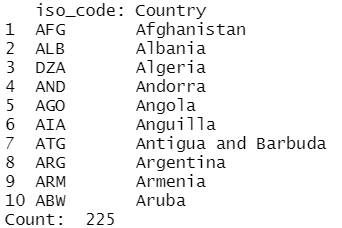
\includegraphics[scale=0.7]{i/i2.png}
        \end{center}
        \vspace{+3mm}\caption{\it Số lượng đất nước và định danh của mỗi đất nước}
    \end{figure}
    
    
\item Số lượng châu lục trong tập mẫu
    \begin{center}
      \begin{tabular}{ c l }
        Continent : & Số châu lục \\ 
        Africa: & Châu phi \\ 
        Asia: & Châu Á \\
      \end{tabular}
    \end{center}

Chúng ta lấy dữ liệu từ cột $continent$ từ tệp gốc rồi loại bỏ những dữ liệu trống, đồng thời sắp xếp, đếm, phiên dịch cùng liệt kê dữ liệu trong đó.
\begin{lstlisting}
i3<-function()
{
  Con <- dataFile %>% select(continent)
  Con<-unique(Con)
  Con <- Con[Con != ""]
  Con<-sort(Con, decreasing = FALSE)
  Trans<-c("Chau Phi", "Chau A", "Chau Au", "Nam My", "Chau Dai Duong", "Bac My")
  m<-data.frame(unlist(Con),unlist(Trans),stringsAsFactors = FALSE)
  colnames(m)<-c("Continent:","6")
  rownames(m)<-c("1","2","3","4","5","6")
  prmatrix(m, left = TRUE, quote = FALSE)
}
i3()
\end{lstlisting}
Kết quả
    \begin{figure}[H]
        \begin{center}
            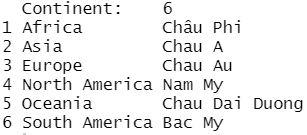
\includegraphics[scale=0.7]{i/i3.png}
        \end{center}
        \vspace{+3mm}\caption{\it Số lượng châu lục trong tập mẫu}
    \end{figure}
    
\item Số lượng dữ liệu thể hiện thu thập dữ liệu được trong từng từng châu lục và tổng số
    \begin{center}
      \begin{tabular}{ c l }
        Continent: & Observations \\ 
        Africa & value1  \\ 
        Asia & value2 \\
        Tổng: & giá trị tổng
      \end{tabular}
    \end{center}

Chúng ta nhóm dữ liệu theo $continent$, sau đó đếm số lượng dòng có trong $continent$, số dòng bằng số dữ liệu thu thập được. Từ đó ta tổng hợp thành một dataframe mới.
\begin{lstlisting}
i4<-function()
{
  formatedData <- dataFile %>% filter(nchar(as.character(continent))>0)
  table <- formatedData %>% group_by(continent) %>% summarise(observation = length(continent))
  ti4<-sum(table$observation)
  a<-c("Tong:",ti4)
  table<-rbind(table,a)
  rownames(table)<-c("1","2","3","4","5","6","7")
  prmatrix(table, left = TRUE, quote = FALSE)
  return(table)
}
table<-i4()
\end{lstlisting}
Kết quả
    \begin{figure}[H]
        \begin{center}
            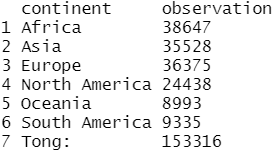
\includegraphics[scale=0.7]{i/i4.png}
        \end{center}
        \vspace{+3mm}\caption{\it Số lượng dữ liệu thu thập được trong từng từng châu lục và tổng số}
    \end{figure}
    
\item Số lượng dữ liệu thể hiện thu thập dữ liệu được trong từng từng đất nước (hiển thị 10 dất nước cuối cùng) và tổng số
    \begin{center}
      \begin{tabular}{ c l }
        iso\_code & Observations \\ 
        AFG & value1  \\ 
        OWID\_AFR & value2 \\
        ALB & value3\\
        Tổng: & giá trị tổng
      \end{tabular}
    \end{center}

Tương tự như câu 4 nhưng chúng ta lấy dữ liệu theo $location$ và xuất ra 10 đất nước (theo isocode) cuối cùng. 
\begin{lstlisting}
i5<-function()
{
  formatedData <- dataFile %>% filter(nchar(as.character(continent))>0)
  table2 <- formatedData %>% group_by(iso_code) %>% summarise(observation = length(iso_code))
  table2.1<-table2[216:225,c(1,2)]
  ti5 <- sum(table2$observation)
  total<-c("Tong:",ti5)
  table2.1<-rbind(table2.1,total)
  rownames(table2.1)<-c("1","2","3","4","5","6","7","8","9","10","11")
  prmatrix(table2.1, left = TRUE, quote = FALSE)
  return(table2<- formatedData %>% group_by(iso_code, location) %>% summarise(observation = length(iso_code)))
}
i5data <-i5()
\end{lstlisting}
Kết quả
    \begin{figure}[H]
        \begin{center}
            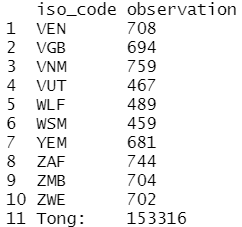
\includegraphics[scale=0.7]{i/i5.png}
        \end{center}
        \vspace{+3mm}\caption{\it Số lượng dữ liệu thu thập được trong từng từng đất nước (hiển thị 10 đất nước cuối cùng) và tổng số}
    \end{figure}
\item Cho biết các châu lục nào có lượng dữ liệu thu thập nhỏ nhất và giá trị nhó nhất đó? 

Từ bảng dữ liệu ở câu 4, ta sử dụng hàm $min()$ để tìm giá trị nhỏ nhất giữa các châu lục
\begin{lstlisting}
i6<-function(table)
{
  mini6<-min(as.numeric(table$observation))
  tmini6 <- table %>% filter(observation == min(as.numeric(observation)))
  cat("Chau luc co luong thu thap du lieu nho nhat la",tmini6$continent,"va gia tri nho nhat do la",tmini6$observation)
}
i6(table)
\end{lstlisting}
Kết quả
\begin{lstlisting}
> i6()
Chau luc co luong thu thap du lieu nho nhat la Oceania va gia tri nho nhat do la 8993
\end{lstlisting}
\item Cho biết các châu lục nào có lượng dữ liệu thu thập lớn nhất và giá trị lớn nhất đó? 

Từ bảng dữ liệu ở câu 4, ta sử dụng hàm $max()$ để tìm giá trị lớn nhất giữa các châu lục
\begin{lstlisting}
i7<-function(table)
{
  cuttable<-table[1:6,c(1,2)]
  maxi7<-max(as.numeric(cuttable$observation))
  tmaxi7 <- cuttable %>% filter(observation == max(as.numeric(observation)))
  cat("Chau luc co luong thu thap du lieu lon nhat la",tmaxi7$continent,"va gia tri lon nhat do la",tmaxi7$observation)
}
i7(table)
\end{lstlisting}
Kết quả
\begin{lstlisting}
> i7()
Chau luc co luong thu thap du lieu lon nhat la Africa va gia tri lon nhat do la 38647
\end{lstlisting}
\item  Cho biết các nước nào có lượng dữ liệu thu thập nhỏ nhất và giá trị nhó nhất đó? 

Từ bảng dữ liệu ở câu 5, ta tìm giá trị thu thập dữ liệu nhỏ nhất, sau đó tìm $isocode$ tương ứng, đồng thời ta tìm được tên quốc gia tương ứng với giá trị nhỏ nhất đó.
\begin{lstlisting}
i8<-function(i5data)
{
  minData <- min(as.numeric(i5data$observation))
  i8result <- i5data %>% filter (as.numeric(observation)==minData)
  colnames(i8result)<-c("iso_code","Country Name", "Min observation")
  i8result<-i8result[c(2,3)]
  prmatrix(i8result, left = TRUE, quote = FALSE)
}
i8(i5data)
\end{lstlisting}
Kết quả
\begin{lstlisting}
> i8(i5data)
     Country Name Min observation
[1,] Pitcairn     85     
\end{lstlisting}
\item Cho biết các nước nào có lượng dữ liệu thu thập lớn nhất và giá trị lớn nhất đó? 

Tương tự câu 8 nhưng chúng ta tìm giá trị lớn nhất.
\begin{lstlisting}
i9<-function(i5data)
{
  maxData <- max(as.numeric(i5data$observation))
  i9result <- i5data %>% filter (as.numeric(observation)==maxData)
  colnames(i9result)<-c("iso_code","Country Name","Max observation")
  i9result<-i9result[c(2,3)]
  prmatrix(i9result, left = TRUE, quote = FALSE)
}
i9(i5data)
\end{lstlisting}
Kết quả
\begin{lstlisting}
> i9(i5data)
     Country Name Max observation
[1,] Argentina    781            
[2,] Mexico       781    
\end{lstlisting}

\item Cho biết các date nào có lượng dữ liệu thu thập nhỏ nhất và giá trị nhó nhất đó? 

Đầu tiên chúng ta sẽ tạo một bảng số liệu thống kê dữ liệu theo ngày, sau đó dựa vào bảng số liệu trên để tìm ra ngày có lượng dữ liệu thu thập nhỏ nhất.
\begin{lstlisting}
dte <- table(dataFile$date)
dte <- as.data.frame(dte)
dte_min <- dte$Var1[dte$Freq==min(dte$Freq)]
cat("Cac ngay co luong du lieu thu thap nho nhat la: ", levels(droplevels(dte_min)), "\n")
cat("Luong du lieu thu thap nho nhat la: ", min(dte$Freq), "\n")
\end{lstlisting}
Kết quả
\begin{lstlisting}
> i10 ()
Cac ngay co luong du lieu thu thap nho nhat la:  1/23/2020 2/18/2020
Luong du lieu thu thap nho nhat la:  10 
\end{lstlisting}

\item Cho biết các date nào có lượng dữ liệu thu thập lớn nhất và giá trị lớn nhất đó? 

Dựa vào bảng số liệu ở câu 10 để tìm ra ngày có lượng dữ liệu thu thập lớn nhất.
\begin{lstlisting}
dte_max <- dte$Var1[dte$Freq==max(dte$Freq)]
cat("Cac ngay co luong du lieu thu thap lon nhat la: ", levels(droplevels(dte_max)), "\n")
cat("Luong du lieu thu thap lon nhat la: ", max(dte$Freq), "\n")
\end{lstlisting}
Kết quả
\begin{lstlisting}
> i11 ()
Cac ngay co luong du lieu thu thap lon nhat la:  1/31/2022 
Luong du lieu thu thap lon nhat la:  196 
\end{lstlisting}

\item Cho biết số lượng dữ liệu thu thập được theo date và châu lục. 

Ta sẽ tổng hợp và đếm số lượng dữ liệu dựa theo ngày và châu lục
\begin{lstlisting}
cont_dte <- table(dataFile$continent, dataFile$date)
cont_dte <- as.data.frame(cont_dte, stringsAsFactors = FALSE)
cont_dte$continent <- cont_dte$Var1
cont_dte$date <- cont_dte$Var2
cont_dte$Number_of_Data <- cont_dte$Freq
cont_dte$Var1 <- NULL
cont_dte$Var2 <- NULL
cont_dte$Freq <- NULL
cont_dte = subset(cont_dte, cont_dte$continent != "")
View(cont_dte)
\end{lstlisting}
Kết quả
    \begin{figure}[H]
        \begin{center}
            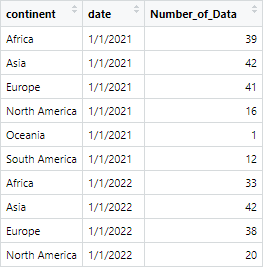
\includegraphics[scale=0.7]{i/i12.png}
        \end{center}
        \vspace{+3mm}\caption{\it Số lượng dữ liệu thu thập được theo ngày và châu lục}
    \end{figure}

\item Cho biết số lượng dữ liệu thu thập được là lớn nhất theo date và châu lục. 

Dựa vào bảng đã tổng hợp từ câu 12, ta có thể tìm được số lượng dữ liệu lớn nhất theo date và châu lục.
\begin{lstlisting}
    cat("So luong du lieu thu thap lon nhat theo date va chau luc la: ", max(cont_dte$Number_of_Data), "\n")
\end{lstlisting}
Kết quả
\begin{lstlisting}
> i13 ()
So luong du lieu thu thap lon nhat theo date va chau luc la:  48
\end{lstlisting}

\item Cho biết số lượng dữ liệu thu thập được là nhỏ nhất theo date và châu lục. 

Tương tự câu 13, dựa vào bảng số liệu ở câu 12, ta có thể tìm được số lượng dữ liệu nhỏ nhất theo date và châu lục.
\begin{lstlisting}
    cat("So luong du lieu thu thap nho nhat theo date va chau luc la: ", min(cont_dte$Number_of_Data), "\n")
\end{lstlisting}
Kết quả
\begin{lstlisting}
> i14 ()
So luong du lieu thu thap nho nhat theo date va chau luc la:  0
\end{lstlisting}

\item Với một date là k và châu lục t cho trước, hãy cho biết số lượng dữ liệu thể hiện thu thập dữ liệu được. 

Dựa vào bảng dữ liệu ở câu 12 ta có thể tìm được số lượng dữ liệu thu thập được trong ngày k ở một châu lục t (VD: Asia ngày 1/1/2021)
\begin{lstlisting}
k = readline()
1/1/2021
t = readline()
Asia
val <- cont_dte$Number_of_Data[(cont_dte$date==k) & (cont_dte$continent==t)]
cat("So luong du lieu thu thap duoc trong ngay",k,"o chau luc",t, "la: ", val, "\n")
\end{lstlisting}
Kết quả
\begin{lstlisting}
> i15 ()
So luong du lieu thu thap duoc trong ngay 1/1/2021 o chau luc Asia la:  42
\end{lstlisting}

\item Có đất nước nào mà số lượng dữ liệu thu thập được là bằng nhau không? Hãy cho biết các iso\_code của đất nước đó. 

Trước tiên từ dữ liệu ban đầu ta sẽ lọc ra những nước có cùng iso\_code và tìm được số lượng dữ liệu thu thập được của mỗi iso\_code, sau đó ta sẽ sắp xếp chúng theo thứ tự tăng dần về số lượng dữ liệu và lọc ra những iso\_code có lượng dữ liệu bằng nhau
\begin{lstlisting}
loc <- table(dataFile$iso_code)
loc <- as.data.frame(loc, stringsAsFactors = FALSE)
country1 <- loc[order(loc$Freq),]
country <- subset(country1, duplicated(Freq) | duplicated(Freq, fromLast = TRUE))
colnames(country) <- c("iso_code", "Num_of_Data")
print(country, row.names = FALSE)
\end{lstlisting}
Kết quả
    \begin{figure}[H]
        \begin{center}
            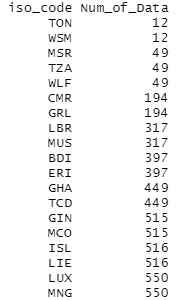
\includegraphics[scale=0.7]{i/i16.png}
        \end{center}
        \vspace{+3mm}\caption{\it iso\_code của các đất nước có lượng dữ liệu thu thập được bằng nhau}
    \end{figure}

\item Liệt kê iso\_code, tên đất nước mà chiều dài iso\_code lớn hơn 3. 

Trước tiên chúng ta sẽ tổng hợp danh sách các iso\_code sau đó lọc ra những nước có chiều dài iso\_code lớn hơn 3.
\begin{lstlisting}
i_c <- table(dataFile$iso_code, dataFile$location)
i_c <- as.data.frame(i_c)
i_l <- subset(i_c, i_c$Freq!=0)
i_l <- as.data.frame(i_l, stringsAsFactors = FALSE)
i <- subset(i_l, str_length(i_l$Var1)>3)
i <- as.data.frame(i)
i$Freq <- NULL
colnames(i) <- c("iso_code", "location")
cat("iso_code cua nhung dat nuoc co do dai iso_code lon hon 3: \n")
print(i, row.names = FALSE)
\end{lstlisting}
Kết quả
    \begin{figure}[H]
        \begin{center}
            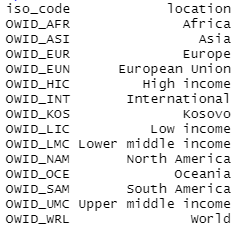
\includegraphics[scale=0.7]{i/i17.png}
        \end{center}
        \vspace{+3mm}\caption{\it Những nước có độ dài iso\_code lớn hơn 3}
    \end{figure}
\end{enumerate}





\subsection{Nhiệm vụ ii}
\begin{enumerate}[ii)]
\item \textcolor{orange}{Nhóm câu hỏi liên quan đến mô tả thống kê cơ bản dữ liệu}
\end{enumerate}

Với mỗi quốc gia mà thuộc về nhóm cần tính số liệu thống kê lần lượt cho nhiễm và tử vong do coronavirus được báo cáo mới:

\begin{enumerate}[1)]

{\bf Xử lý chung}: Trước hết, ta cần trích lọc dữ liệu cần thiết của 3 quốc gia cần xử lý (Indonesia, Japan, Vietnam), để thuận tiện hơn trong khi thực hiện chương trình. Các câu hỏi là tương đương nhau cho mỗi quốc gia, do đó, chúng ta có thể dùng dòng $for$ để xử lý. \\

{\it Lưu ý: Ở phần trình bày câu ii này, ta quy ước số thứ tự 1, 2, 3 lần lượt tương ứng với Indonesia, Japan, Vietnam.}

\begin{lstlisting}
indoFile <- subset(dataFile, dataFile$location == "Indonesia")
japanFile <- subset(dataFile, dataFile$location == "Japan")
vietnamFile <- subset(dataFile, dataFile$location == "Vietnam") 

ii_File <- list(indoFile, japanFile, vietnamFile)
ii_string <- cbind("Indonesia", "Japan", "Vietnam")
\end{lstlisting}

\item Tính giá trị nhỏ nhất, lớn nhất \\
    Chúng ta chỉ cần dùng hàm $min()$, $max()$ đơn giản, với lưu ý là phải bỏ qua các giá trị NA.\\
    Ta cũng tạo sẵn các vector để lưu giá trị của phép tính nhằm thực hiện câu hỏi bên dưới dễ dàng hơn.
    \begin{lstlisting}
cases_min <- vector(length = 3)
cases_max <- vector(length = 3)
deaths_min <- vector(length = 3)
deaths_max <- vector(length = 3)
    
for (i in 1:3) {
  cases_min[i] = min(na.omit(data.frame(ii_File[i])$new_cases))
  cases_max[i] = max(na.omit(data.frame(ii_File[i])$new_cases))
  deaths_min[i] = min(na.omit(data.frame(ii_File[i])$new_deaths))
  deaths_max[i] = max(na.omit(data.frame(ii_File[i])$new_deaths))
  cat(ii_string[i], "min new cases =", cases_min[i], "\n")
  cat(ii_string[i], "max new cases =", cases_max[i], "\n")
  cat(ii_string[i], "min new deaths =", deaths_min[i], "\n")
  cat(ii_string[i], "max new deaths =", deaths_max[i], "\n", "\n")
}
    \end{lstlisting}
    Kết quả
    \begin{figure}[H]
        \begin{center}
            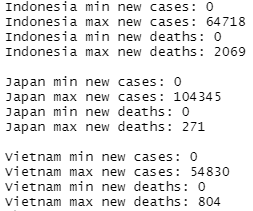
\includegraphics[scale=0.7]{ii/max min.png}
        \end{center}
        \vspace{+3mm}\caption{\it Giá trị lớn nhất, nhỏ nhất}
    \end{figure}
    
    
\item Tính tứ phân vị thứ nhất(Q1), thứ hai(Q2), thứ ba(Q3)\\
    Để gọn gàng, ở những phần tiếp theo trong câu ii này, bài viết sẽ không trình bày những dòng lệnh tương tự với nhau nữa.\\
    Để tính tứ phân vị, chúng ta sử dụng hàm $quantile()$. Hàm này sẽ trả về cả 5 giá trị tứ phân vị, nên ta chỉ cần lấy các giá trị thứ 2, 3, 4 tương ứng với Q1, Q2, Q3.
    \begin{lstlisting}
cases_Q1 <- vector(length = 3)
    
for (i in 1:3) {
  cases_Q1[i] = unname(quantile(na.omit(data.frame(ii_File[i])$new_cases))[2])
  cat(ii_string[i], "Q1 new cases =", cases_Q1[i], "\n")
}
    \end{lstlisting}
    
    Kết quả
    \begin{figure}[H]
        \begin{center}
            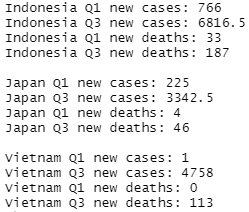
\includegraphics[scale=0.7]{ii/quantile.png}
        \end{center}
        \vspace{+3mm}\caption{\it Giá trị tứ phân vị}
    \end{figure}
    
\item Tính giá trị trung bình (Avg)\\
    Chúng ta sử dụng hàm $mean()$ và bỏ qua các giá trị NA để tính giá trị trung bình.
    
    \begin{lstlisting}
cases_avg <- vector(length = 3)

for (i in 1:3) {
  cases_avg[i] = mean(na.omit(data.frame(ii_File[i])$new_cases))
  cat(ii_string[i], "average new cases =", cases_avg[i], "\n")
}
    \end{lstlisting}
    
        Kết quả
    \begin{figure}[H]
        \begin{center}
            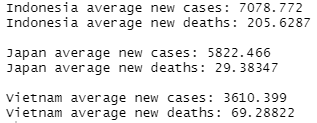
\includegraphics[scale=0.7]{ii/avg.png}
        \end{center}
        \vspace{+3mm}\caption{\it Giá trị trung bình}
    \end{figure}
    
    
\item Tính giá trị độ lệch chuẩn (Std)\\
    Chúng ta sử dụng hàm $sd()$ và bỏ qua các giá trị NA để tính độ lệch chuẩn.
    
    \begin{lstlisting}
cases_std <- vector(length = 3)

for (i in 1:3) {
  cases_std[i] = sd(na.omit(data.frame(ii_File[i])$new_cases))
  cat(ii_string[i], "standard deviation new cases =", cases_std[i], "\n")
}
    \end{lstlisting}
    
        Kết quả
    \begin{figure}[H]
        \begin{center}
            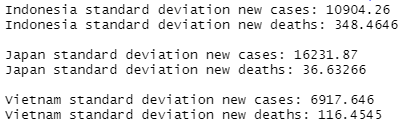
\includegraphics[scale=0.7]{ii/sd.png}
        \end{center}
        \vspace{+3mm}\caption{\it Giá trị độ lệch chuẩn}
    \end{figure}


\item Đếm xem có bao nhiêu outliers, một quan sát mà giá trị của nó nằm trong khoảng sau:\\
$IQR = Q3 - Q1$\\
$outliers < Q1 - 1.5*IQR$ hoặc $outliers > Q3 + 1.5*IQR$\\
    Với giá trị Q1, Q3 đã tính ở câu trên, ta dễ dàng tính được giá trị IQR. Sau đó kết hợp $subset()$ để trích xuất dữ liệu thỏa mãn outlier và $nrow()$ để xác định số hàng trong $subset$ vừa thực hiện.
    
    \begin{lstlisting}
cases_outlier <- vector(length = 3)

for (i in 1:3) {
  cases_IQR = cases_Q3[i] - cases_Q1[1] 
  cases_outlier[i] = nrow(subset(data.frame(ii_File[i]), 
  new_cases < cases_Q1[i] - 1.5*cases_IQR | 
  new_cases > cases_Q3[i] + 1.5*cases_IQR))
  
  cat(ii_string[i], "outliers new cases =", cases_outlier[i], "\n")
}
    \end{lstlisting}
    
        Kết quả
    \begin{figure}[H]
        \begin{center}
            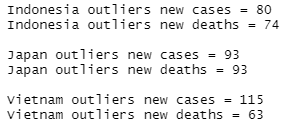
\includegraphics[scale=0.7]{ii/outliers.png}
        \end{center}
        \vspace{+3mm}\caption{\it Số lượng outlier}
    \end{figure}
    
    

\item Lập bảng mô tả số liệu thống kê cho từng đất nước thuộc về nhóm: 
    \begin{center}
        \begin{tabular}{ c c c c c c c c c}
            Countries & Min & Q1 & Q2 & Q3 & Max & Avg & Std & Outlier \\ 
            ctr\_i & ? & ? & ? & ? & ? & ? & ? & ? \\ 
        \end{tabular}
    \end{center}
    Chúng ta lập bảng bằng cách sử dụng $cbind()$ và $rbind()$ để kết hợp các dữ liệu lại với nhau.
    
    \begin{lstlisting} 
cases_table <- vector()
for (i in 1:3) {
  cases_table = rbind(cases_table, cbind("Countries" = ii_string[i],
  "Min"=cases_min[i], "Q1"=cases_Q1[i], "Q2"=cases_Q2[i], 
  "Q3"=cases_Q3[i], "Max"=cases_max[i], "Avg"=cases_avg[i], 
  "Std"=cases_std[i], "Outlier"=cases_outlier[i]))
}

\end{lstlisting}

    Kết quả
    \begin{figure}[H]
        \begin{center}
            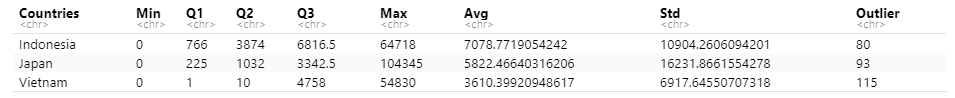
\includegraphics[scale=0.6]{ii/cases_table.png}
            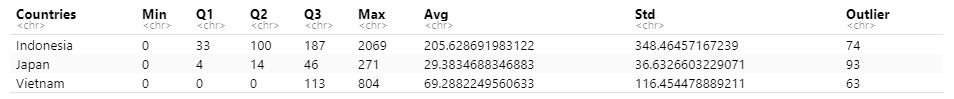
\includegraphics[scale=0.6]{ii/deaths_table.png}
        \end{center}
        \vspace{+3mm}\caption{\it Bảng số liệu new cases (phía trên) và new deaths (phía dưới)}
    \end{figure}

\item Vẽ biểu đồ boxplot hay còn được gọi là box-and-whisker cho nhiễm coronavirus \\
Rất rõ ràng, chúng ta sử dụng hàm $boxplot()$ để vẽ biểu đồ boxplot cho dữ liệu.

\begin{lstlisting}
for (i in 1:3) {
  boxplot(data.frame(ii_File[i])$new_cases, main=paste(ii_string[i], "new_cases boxplot"))
  boxplot(data.frame(ii_File[i])$new_deaths, main=paste(ii_string[i], "new_deaths boxplot"))
}
\end{lstlisting}

    Kết quả
    \begin{figure}[H]
        \begin{center}
            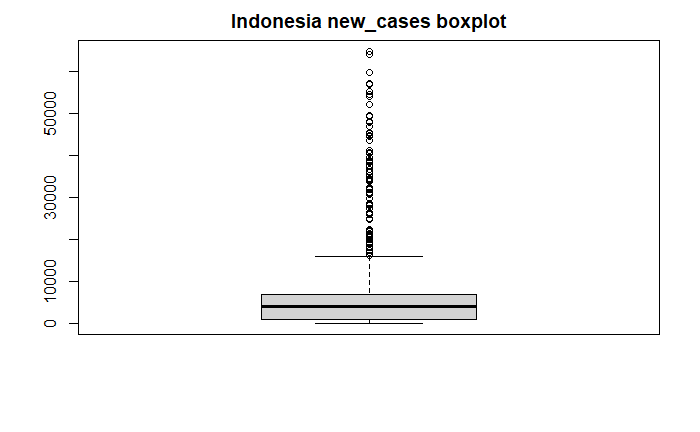
\includegraphics[scale=0.4]{ii/indo box cases.png}
            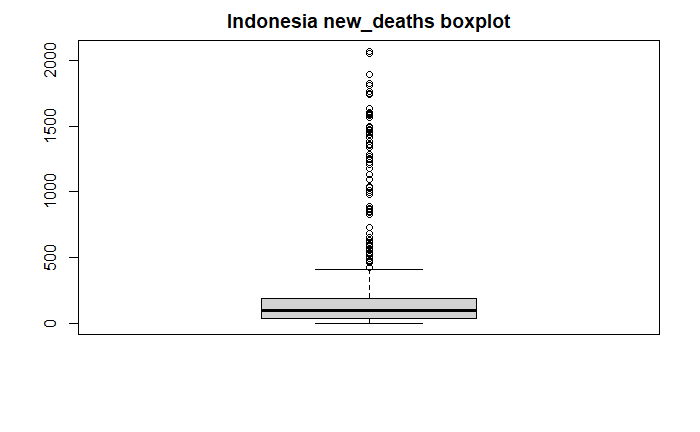
\includegraphics[scale=0.4]{ii/indo box deaths.png}
        \end{center}
    \end{figure}
    \begin{figure}[H]
        \begin{center}
            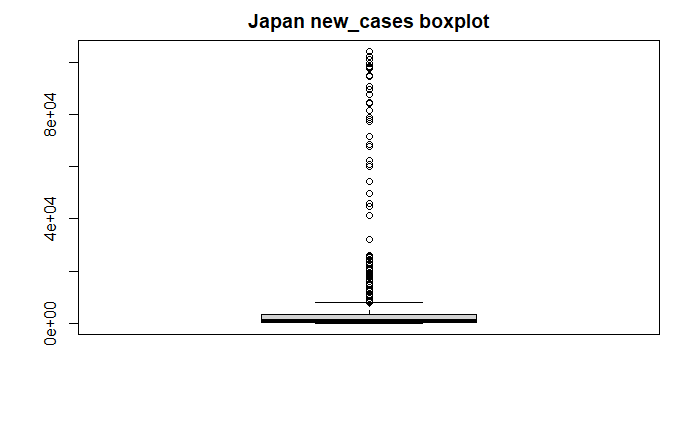
\includegraphics[scale=0.4]{ii/japan box cases.png}
            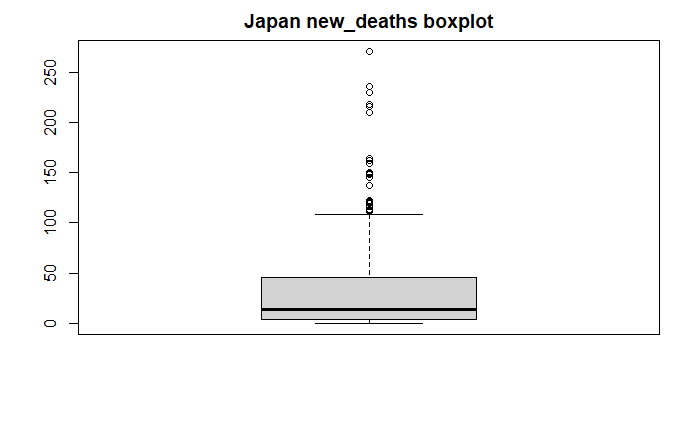
\includegraphics[scale=0.4]{ii/japan box deaths.png}
        \end{center}
    \end{figure}
    \begin{figure}[H]
        \begin{center}
            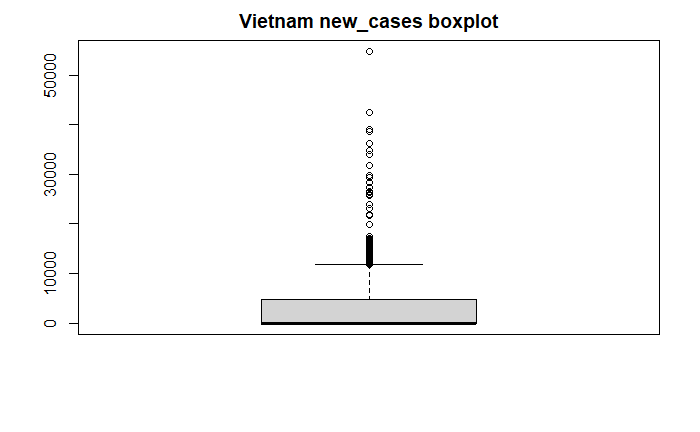
\includegraphics[scale=0.4]{ii/vietnam box cases.png}
            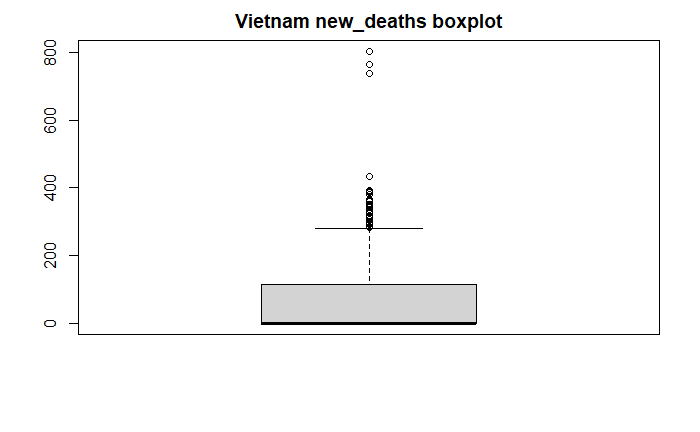
\includegraphics[scale=0.4]{ii/vietnam box deaths.png}
        \end{center}
        \vspace{+3mm}\caption{\it Biểu đồ boxplot của new cases và new deaths}
    \end{figure}
%%%%%%%%%%%%%%%%%%%%%%%%%%%%%%%%%%%%
\end{enumerate}










\subsection{Nhiệm vụ iii}
\begin{enumerate}[iii)]
\item \textcolor{orange}{Nhóm câu hỏi liên quan đến dữ liệu thể hiện thu thập dữ liệu}
\end{enumerate}

Với mỗi quốc gia mà thuộc về nhóm cần tính số liệu thống kê lần lượt cho nhiễm và tử vong do coronavirus:

\textbf{Xử lí chung:} Đầu tiên chúng ta nhập dữ liệu vào bảng, sửa những giá trị âm lại thành giá trị dương và sau đó lọc tiếp dữ liệu của từng nước cần được xử lí ra bảng.\\
Vì câu hỏi tính số liệu thống kê lần lượt cho nhiễm và tử vong như nhau (trừ câu 7 và 8) nên báo cáo chỉ giới thiệu về cách xử lí đối với lượt nhiễm; làm tương tự đối với lượt tử vong.

\begin{lstlisting}
dataFile <- read_csv("owid-covid-data.csv", show_col_types = FALSE)
  
# convert negative entries to positive
dataFile$new_cases <- abs(dataFile$new_cases)
dataFile$new_deaths <- abs(dataFile$new_deaths)
  
# separate country from database
dataFile_ISO <- subset(dataFile, iso_code==country_code)
\end{lstlisting}

\begin{enumerate}[1)]
    \item Có bao nhiêu ngày có số lần dữ liệu không được báo cáo mới.
    
    Từ bảng dữ liệu cho từng nước, ta lọc ra các ngày có dữ liệu được báo cáo hợp lệ (khác 0 và khác NA), sau đó loại những ngày hợp lệ ra khỏi bảng dữ liệu chung của nước đó, ta được bảng những ngày không được báo cáo mới.
    
    \begin{lstlisting}[gobble=4]
    dataFile_cases <- subset(dataFile_ISO, dataFile_ISO$new_cases>0)
    invalid_cases <- subset(dataFile_ISO, !(new_cases %in% dataFile_cases$new_cases) |    is.na(new_cases), select = c(location, new_cases, new_deaths))
    cat("1. So ngay du lieu khong duoc bao cao moi:", nrow(invalid_cases), "ngay \n")
    \end{lstlisting}
    
    \item Có bao nhiêu ngày có số ca nhiễm/ tử vong là thấp nhất được báo cáo mới.
    
    Từ bảng dữ liệu được báo cáo hợp lệ, ta  tìm số ca nhiễm trong ngày thấp nhất rồi thống kê xem có bao nhiêu ngày có số ca nhiễm bằng với số ca vừa tìm được.
    
    \begin{lstlisting}[gobble=4]
    cases_min <- min(dataFile_cases$new_cases)
    cases_min_Freq <- table(dataFile_ISO$new_cases==cases_min)
    cat("2. So ngay co so ca nhiem thap nhat:", unname(cases_min_Freq["TRUE"]), "\n")
    \end{lstlisting}
    
    \item Có bao nhiêu ngày có số ca nhiễm/ tử vong là cao nhất được báo cáo mới
    
    Từ bảng dữ liệu được báo cáo hợp lệ, ta  tìm số ca nhiễm trong ngày cao nhất rồi thống kê xem có bao nhiêu ngày có số ca nhiễm bằng với số ca vừa tìm được.
    
    \begin{lstlisting}[gobble=4]
    cases_max <- max(dataFile_cases$new_cases)
    cases_max_Freq <- table(dataFile_ISO$new_cases==cases_max)
    cat("3. So ngay co so ca nhiem cao nhat:", unname(cases_max_Freq["TRUE"]), "\n")
    \end{lstlisting}
    
    \item Thể hiện bảng số liệu như sau:\\
    Không được báo cáo mới
    \begin{center}
      \begin{tabular}{ c c c }
        Countries & Infections & Deaths \\ 
        ctr\_i & value  & value\\ 
      \end{tabular}
    \end{center}
    Báo cáo mới:
    \begin{center}
      \begin{tabular}{ c c c }
        Countries & Infections & Deaths \\ 
        ctr\_i & value  & value\\ 
      \end{tabular}
    \end{center}
    Không được báo cáo mới: Xuất ra bảng những ngày không có báo cáo mới (ở câu 1)
    \begin{lstlisting}[gobble=4]
    colnames(invalid_cases) <- c("Countries", "Infections", "Deaths")
    cat("4. \nKhong duoc bao cao moi: \n") 
    print(invalid_cases)
    \end{lstlisting}
    Báo cáo mới: Từ bảng dữ liệu chung của từng nước, kết hợp với số ca thấp nhât/cao nhất tìm được ở câu 2) và 3), chúng ta tạo bảng gồm những ngày có số ca nhiễm thấp nhất và cao nhất, sau đó xuất bảng ra màn hình.
    \begin{lstlisting}[gobble=4]
    min_max_cases <- subset(dataFile_ISO, new_cases==cases_min | new_cases==cases_max, select = c(location, new_cases, new_deaths))
    colnames(min_max_cases) <- c("Countries", "Infections", "Deaths")
    cat("\nBao cao moi: \n")
    print(min_max_cases)
    \end{lstlisting}
    
    \item Cho biết số ngày ngắn nhất liên tiếp mà không có dữ liệu được báo cáo\\
    Hướng giải quyết: Tìm chuỗi ngày ngắn nhất mà có số ca nhiễm bằng NA\\
    Trong R: Tạo một hàm mới $condition\_NA$ xác định xem ngày hôm đó số ca nhiễm có phải NA hay không (hàm trả về $TRUE$ hoặc $FALSE$), sau đó áp dụng hàm lên toàn bộ cột $new\_cases$ của bảng dữ liệu của từng nước. Ta được một chuỗi kí tự bao gồm $TRUE$ và $FALSE$ nối tiếp với nhau, tương ứng với kết quả trả về của hàm. Sau đó dùng hàm $rle$ để thống kê số lần xuất hiện liên tiếp của từng kết quả ($TRUE$ hoặc $FALSE$). Cuối cùng ta tìm giá trị nhỏ nhất của số lần xuất hiện $TRUE$.
    \begin{lstlisting}[gobble=4]
    condition_NA <- function(x) is.na(x)
    dataFile_cases_NA <- rle(condition_NA(dataFile_ISO$new_cases))
    cases_NA_minFreq <- min(dataFile_cases_NA$lengths[dataFile_cases_NA$values == TRUE], na.rm = TRUE)
    # checks if NA, Inf/-Inf or NaN -> resets to 0
    cases_NA_minFreq[!is.finite(cases_NA_minFreq)] <- 0
    cat("5. So ngay ngan nhat lien tiep khong co du lieu duoc bao cao:", cases_NA_minFreq,"\n")
    \end{lstlisting}
    \item Cho biết số ngày dài nhất liên tiếp mà không có dữ liệu được báo cáo\\
    Tương tự câu 5), nhưng chúng ta tìm giá trị lớn nhất của số lần xuất hiện $TRUE$
    \begin{lstlisting}[gobble=4]
    condition_NA <- function(x) is.na(x)
    dataFile_cases_NA <- rle(condition_NA(dataFile_ISO$new_cases))
    cases_NA_maxFreq <- max(dataFile_cases_NA$lengths[dataFile_cases_NA$values == TRUE], na.rm = TRUE)
    # checks if NA, Inf/-Inf or NaN -> resets to 0
    cases_NA_maxFreq[!is.finite(cases_NA_minFreq)] <- 0
    cat("6. So ngay dai nhat lien tiep khong co du lieu duoc bao cao:", cases_NA_maxFreq,"\n")
    \end{lstlisting}
    \item Cho biết số ngày ngắn nhất liên tiếp mà không có người nhiễm bệnh mới\\
    Hướng giải quyết: Tìm chuỗi ngày ngắn nhất mà có số ca nhiễm bằng 0\\
    Trong R: Tạo một hàm mới $condition\_no\_new\_cases$ xác định xem ngày hôm đó số ca nhiễm có bằng 0 hay không (hàm trả về $TRUE$ hoặc $FALSE$). Sau đó thực hiện tương tự như câu 5)
    \begin{lstlisting}[gobble=4]
    condition_no_new_cases <- function(x) x==0
    dataFile_cases_zero <- rle(condition_no_new_cases(dataFile_ISO$new_cases))
    cases_zero_minFreq <- min(dataFile_cases_zero$lengths[dataFile_cases_zero$values == TRUE], na.rm = TRUE)
    # checks if NA, Inf/-Inf or NaN -> resets to 0
    cases_zero_minFreq[!is.finite(cases_zero_minFreq)] <- 0
    cat("7. So ngay ngan nhat lien tiep khong co nguoi nhiem benh moi:", cases_zero_minFreq,"\n")
    \end{lstlisting}
    \item Cho biết số ngày dài nhất liên tiếp mà không có người nhiễm bệnh mới\\
    Tương tự câu 7), nhưng chúng ta tìm giá trị lớn nhất của số lần xuất hiện $TRUE$
    \begin{lstlisting}[gobble=4]
    condition_no_new_cases <- function(x) x==0
    dataFile_cases_zero <- rle(condition_no_new_cases(dataFile_ISO$new_cases))
    cases_zero_maxFreq <- max(dataFile_cases_zero$lengths[dataFile_cases_zero$values == TRUE], na.rm = TRUE)
    # checks if NA, Inf/-Inf or NaN -> resets to 0
    cases_zero_maxFreq[!is.finite(cases_zero_maxFreq)] <- 0
    cat("8. So ngay dai nhat lien tiep khong co nguoi nhiem benh moi:", cases_zero_maxFreq,"\n")
    \end{lstlisting}
\end{enumerate}
Làm tương tự với các nước còn lại cần được xử lí dữ liệu.

\textbf{Kết quả}

\begin{figure}[H]
    \begin{center}
            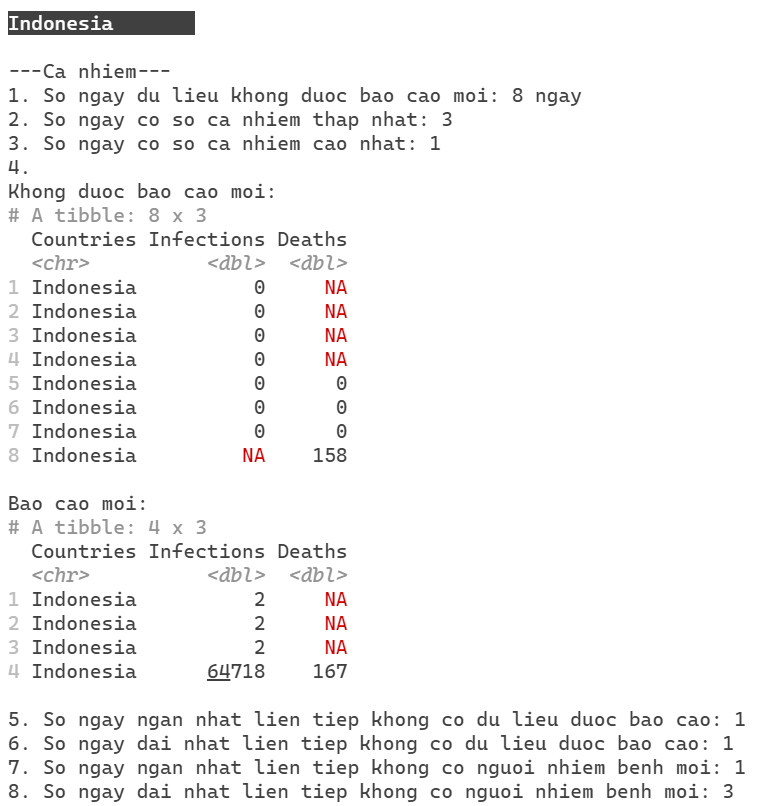
\includegraphics[scale=0.6]{iii/idn_1.png}
    \end{center}
    \caption{\it Kết quả đối với ca nhiễm}
\end{figure}
\begin{figure}[H]
    \begin{center}
            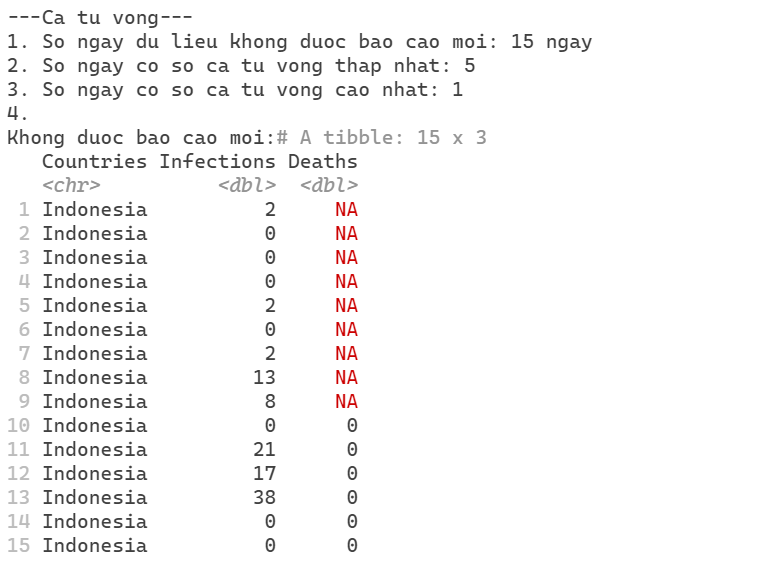
\includegraphics[scale=0.6]{iii/idn_2.png}
    \end{center}
    \caption{\it Kết quả đối với ca tử vong}
\end{figure}
\begin{figure}[H]
    \begin{center}
            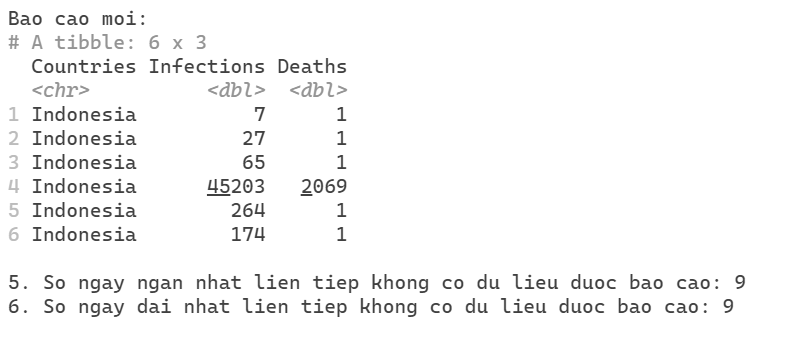
\includegraphics[scale=0.6]{iii/idn_3.png}
    \end{center}
    \caption{\it Kết quả đối với ca tử vong}
\end{figure}









\subsection{Nhiệm vụ iv}
\begin{enumerate}[iv)]
\item \textcolor{red}{Nhóm câu hỏi liên quan đến trực quan dữ liệu}
\end{enumerate}
\begin{enumerate}[1)]
{\bf Xử lý chung cho câu 1 và 2} \\
Chúng ta tính tổng số quốc gia dựa trên châu lục, tính tỉ lệ số đất nước từng châu lục so với số đất nước toàn thế giới rồi đưa chúng vào bảng.
\begin{lstlisting}
Countries <- dataFile %>% select(location)
Con <- dataFile %>% select(continent)
temp<- cbind(Countries,Con)
temp <- distinct(temp)
Countries <- count(temp, 'continent')
probability <- prop.table(Countries[,2])
cumulative <- cumsum(Countries[,2])
Countries <- cbind(Countries, probability,cumulative)
\end{lstlisting}
\item Vẽ biểu đồ tần số tích lũy quốc gia cho các châu lục
\begin{lstlisting}
graph1 <- ggplot(data = Countries, aes(x=continent, y=cumulative)) +
geom_bar(stat = "identity", position = "dodge", fill = "steelblue") +
labs(title = "",x="Continent", y="Cumulative frequence") 

graph1
ggsave("iv.1) Cumulative frequence.png", plot = graph1)
\end{lstlisting}
Kết quả
    \begin{figure}[H]
        \begin{center}
            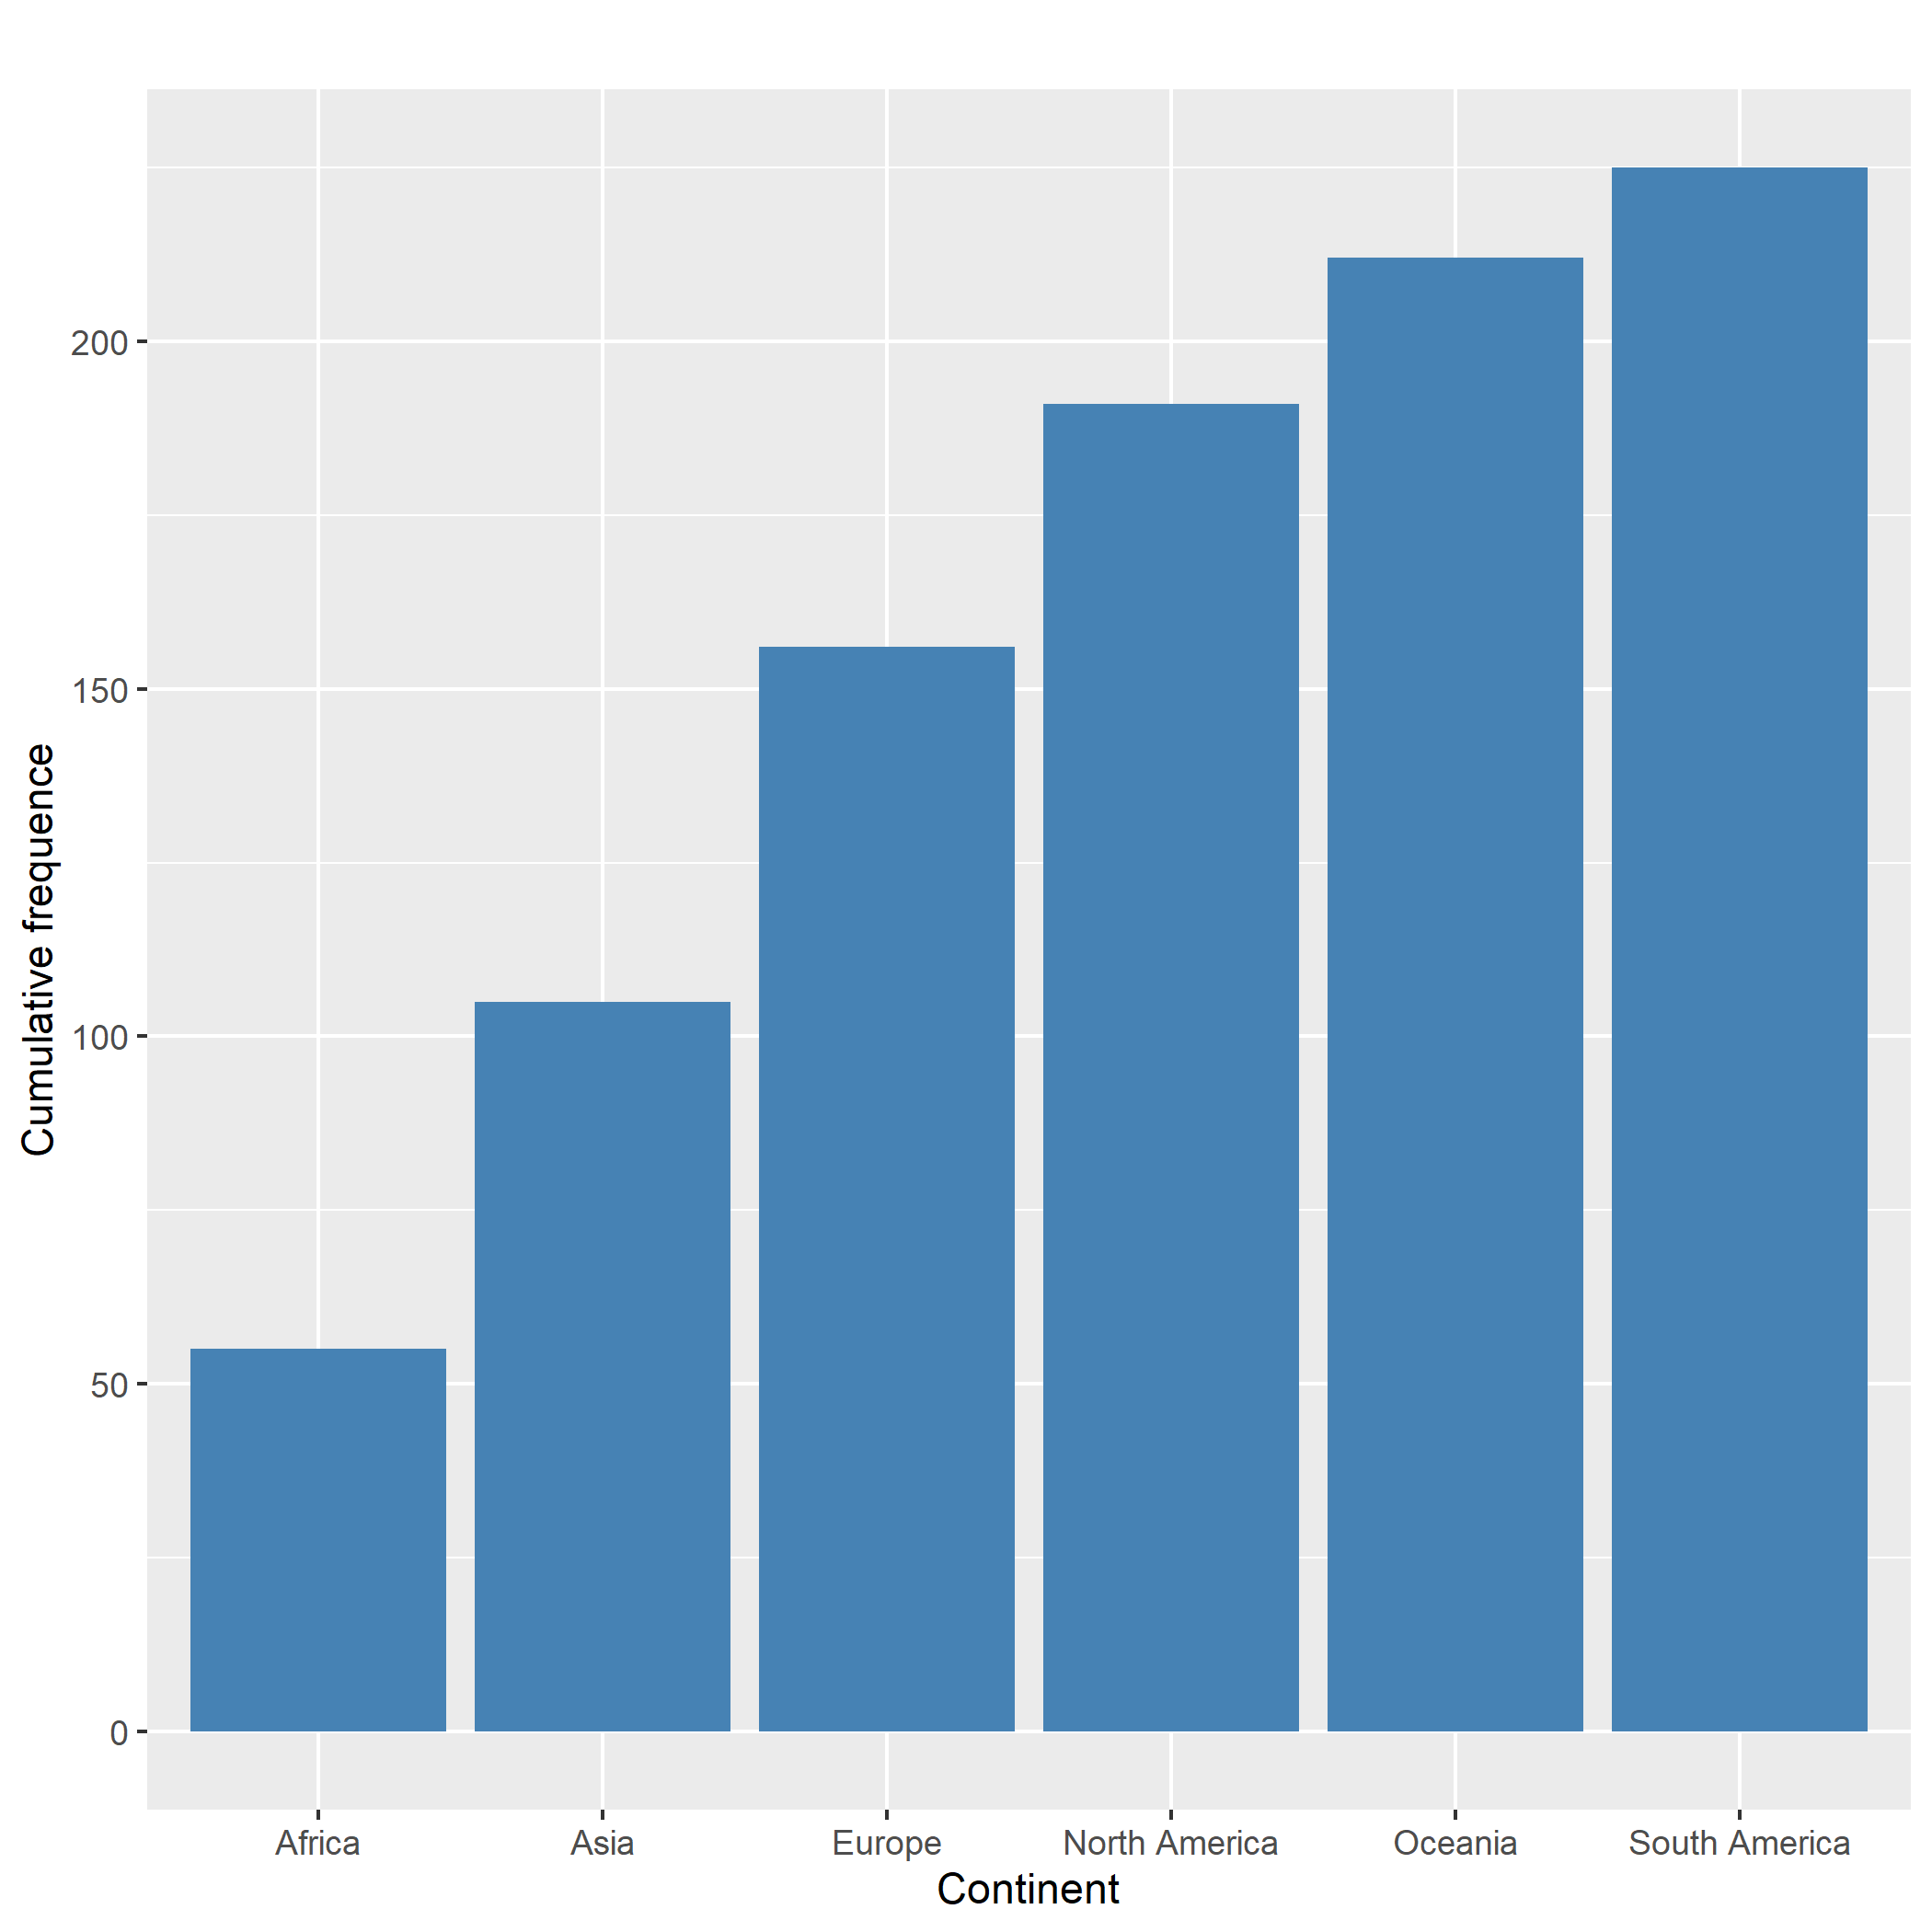
\includegraphics[scale=0.7]{iv/iv.1) Cumulative frequence.png}
        \end{center}
        \vspace{+3mm}\caption{\it Biểu đồ tần số tích lũy quốc gia cho các châu lục}
    \end{figure}
\item Vẽ biểu đồ tần số tương đối quốc gia cho các châu lục
\begin{lstlisting}
graph2 <- ggplot(data = Countries, aes(x=continent, y=probability)) +
  geom_bar(stat = "identity", position = "dodge", fill = "steelblue") +
  labs(title = "",x="Continent", y="Relavtive frequence")

graph2
ggsave("iv.2) Relavtive frequence.png", plot = graph2)
\end{lstlisting}
Kết quả
    \begin{figure}[H]
        \begin{center}
            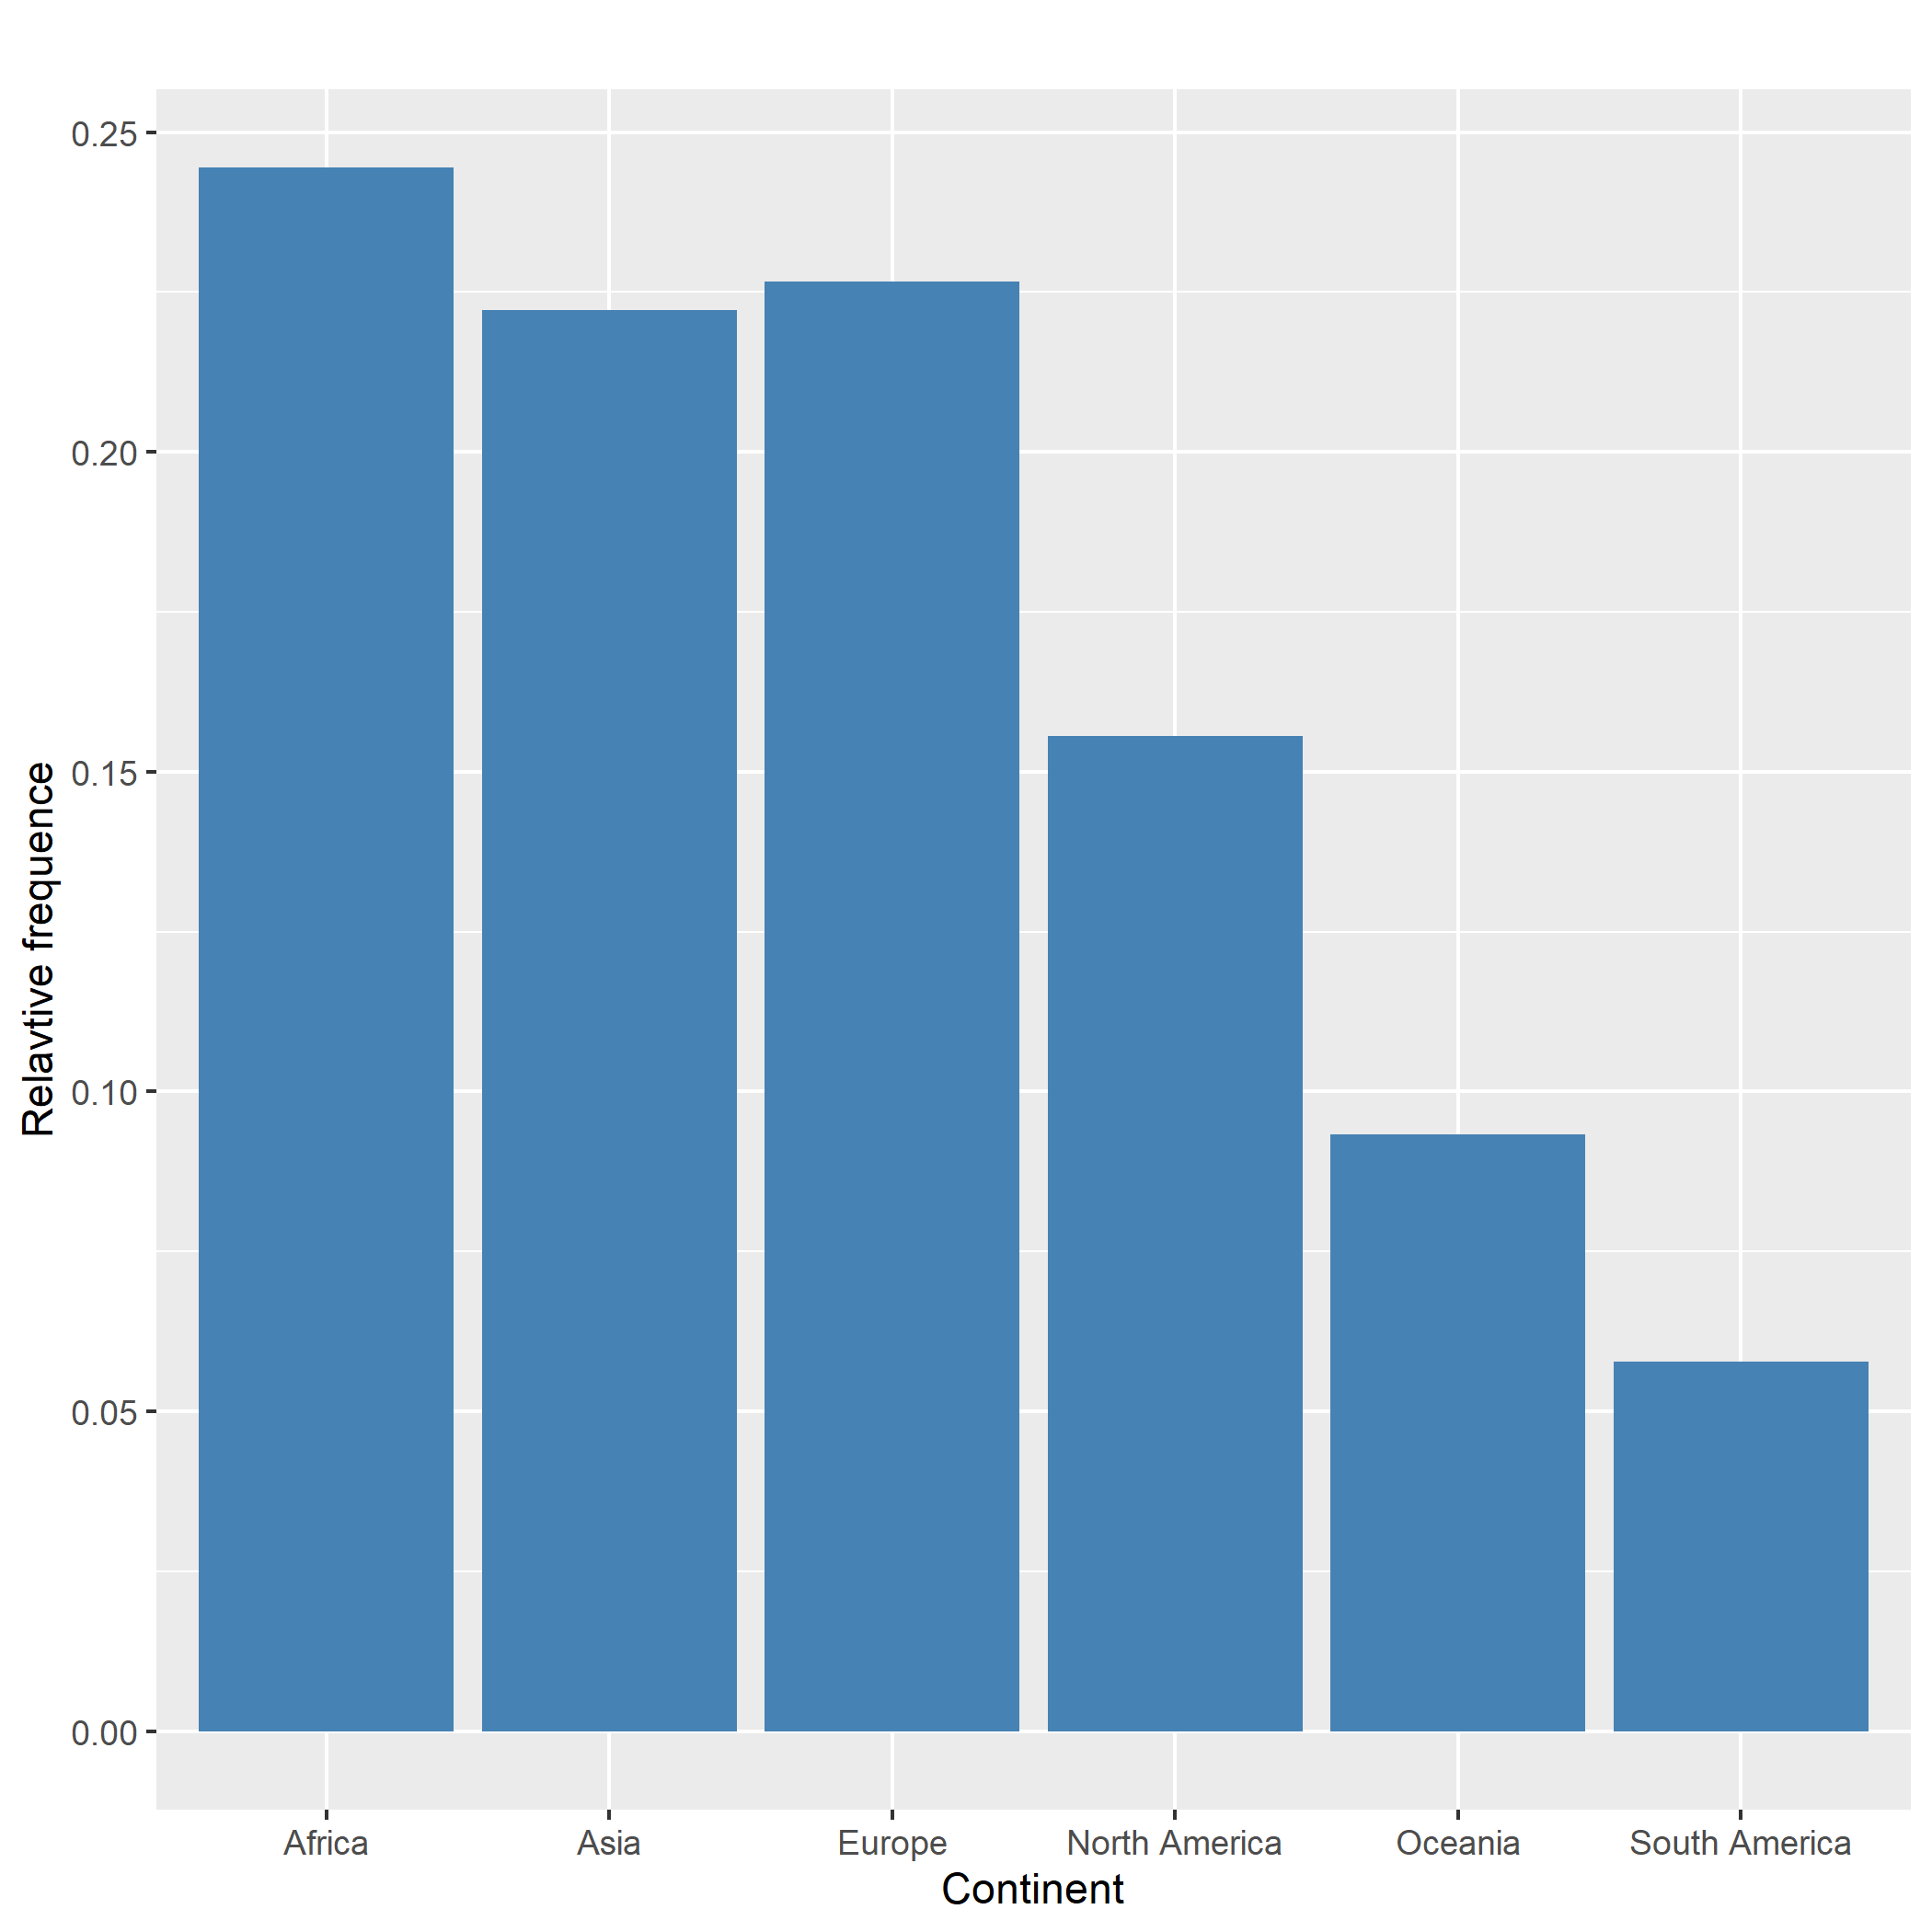
\includegraphics[scale=0.7]{iv/iv.2) Relavtive frequence.png}
        \end{center}
        \vspace{+3mm}\caption{\it Biểu đồ tần số tương đối quốc gia cho các châu lục}
    \end{figure}
    
{\bf Xử lý chung cho câu 3 và 4}  \\
Chúng ta lấy dữ liệu $new cases$ và số $new deaths$ theo quốc gia, cùng với $date$, rồi tách bộ phận dữ liệu gồm 7 ngày cuối cùng của năm cuối cùng của từng quốc gia.
\begin{lstlisting}
dataFile$new_cases <- abs(dataFile$new_cases)
dataFile$new_deaths <- abs(dataFile$new_deaths)
InJaVi <- dataFile %>% filter(location == "Indonesia" | location == "Japan" | location == "Vietnam")
InJaVi <- InJaVi %>% select(location | date | new_cases | new_deaths)

tmp <- InJaVi
formatedDate <- as.Date(tmp$date, format = "%m/%d/%Y")
tmp[,"date"] <-formatedDate

thelastday <- max(formatedDate)
thelastsevendays <- tmp %>% group_by(location) %>% filter(date > thelastday - 7)
\end{lstlisting}
\item Vẽ biểu đồ thể hiện nhiễm bệnh đã báo cáo của các quốc gia trong 7 ngày cuối của năm cuối cùng
\begin{lstlisting}
graph3 <- ggplot(data = thelastsevendays, aes(x = date, y = new_cases, fill = factor(location))) +
  theme_bw() +
  geom_bar(stat = "identity", position = "dodge") +
  labs(title = "New cases for the last 7 days", x = "Date", y = "New Cases") +
  theme(plot.title = element_text(hjust = 0.5)) + scale_fill_manual("Location", values = c("Indonesia" = "black", "Japan" = "red", "Vietnam" = "blue"))

graph3
ggsave("iv.3) New cases for the last 7 days.png", plot = graph3)
\end{lstlisting}
Kết quả
    \begin{figure}[H]
        \begin{center}
            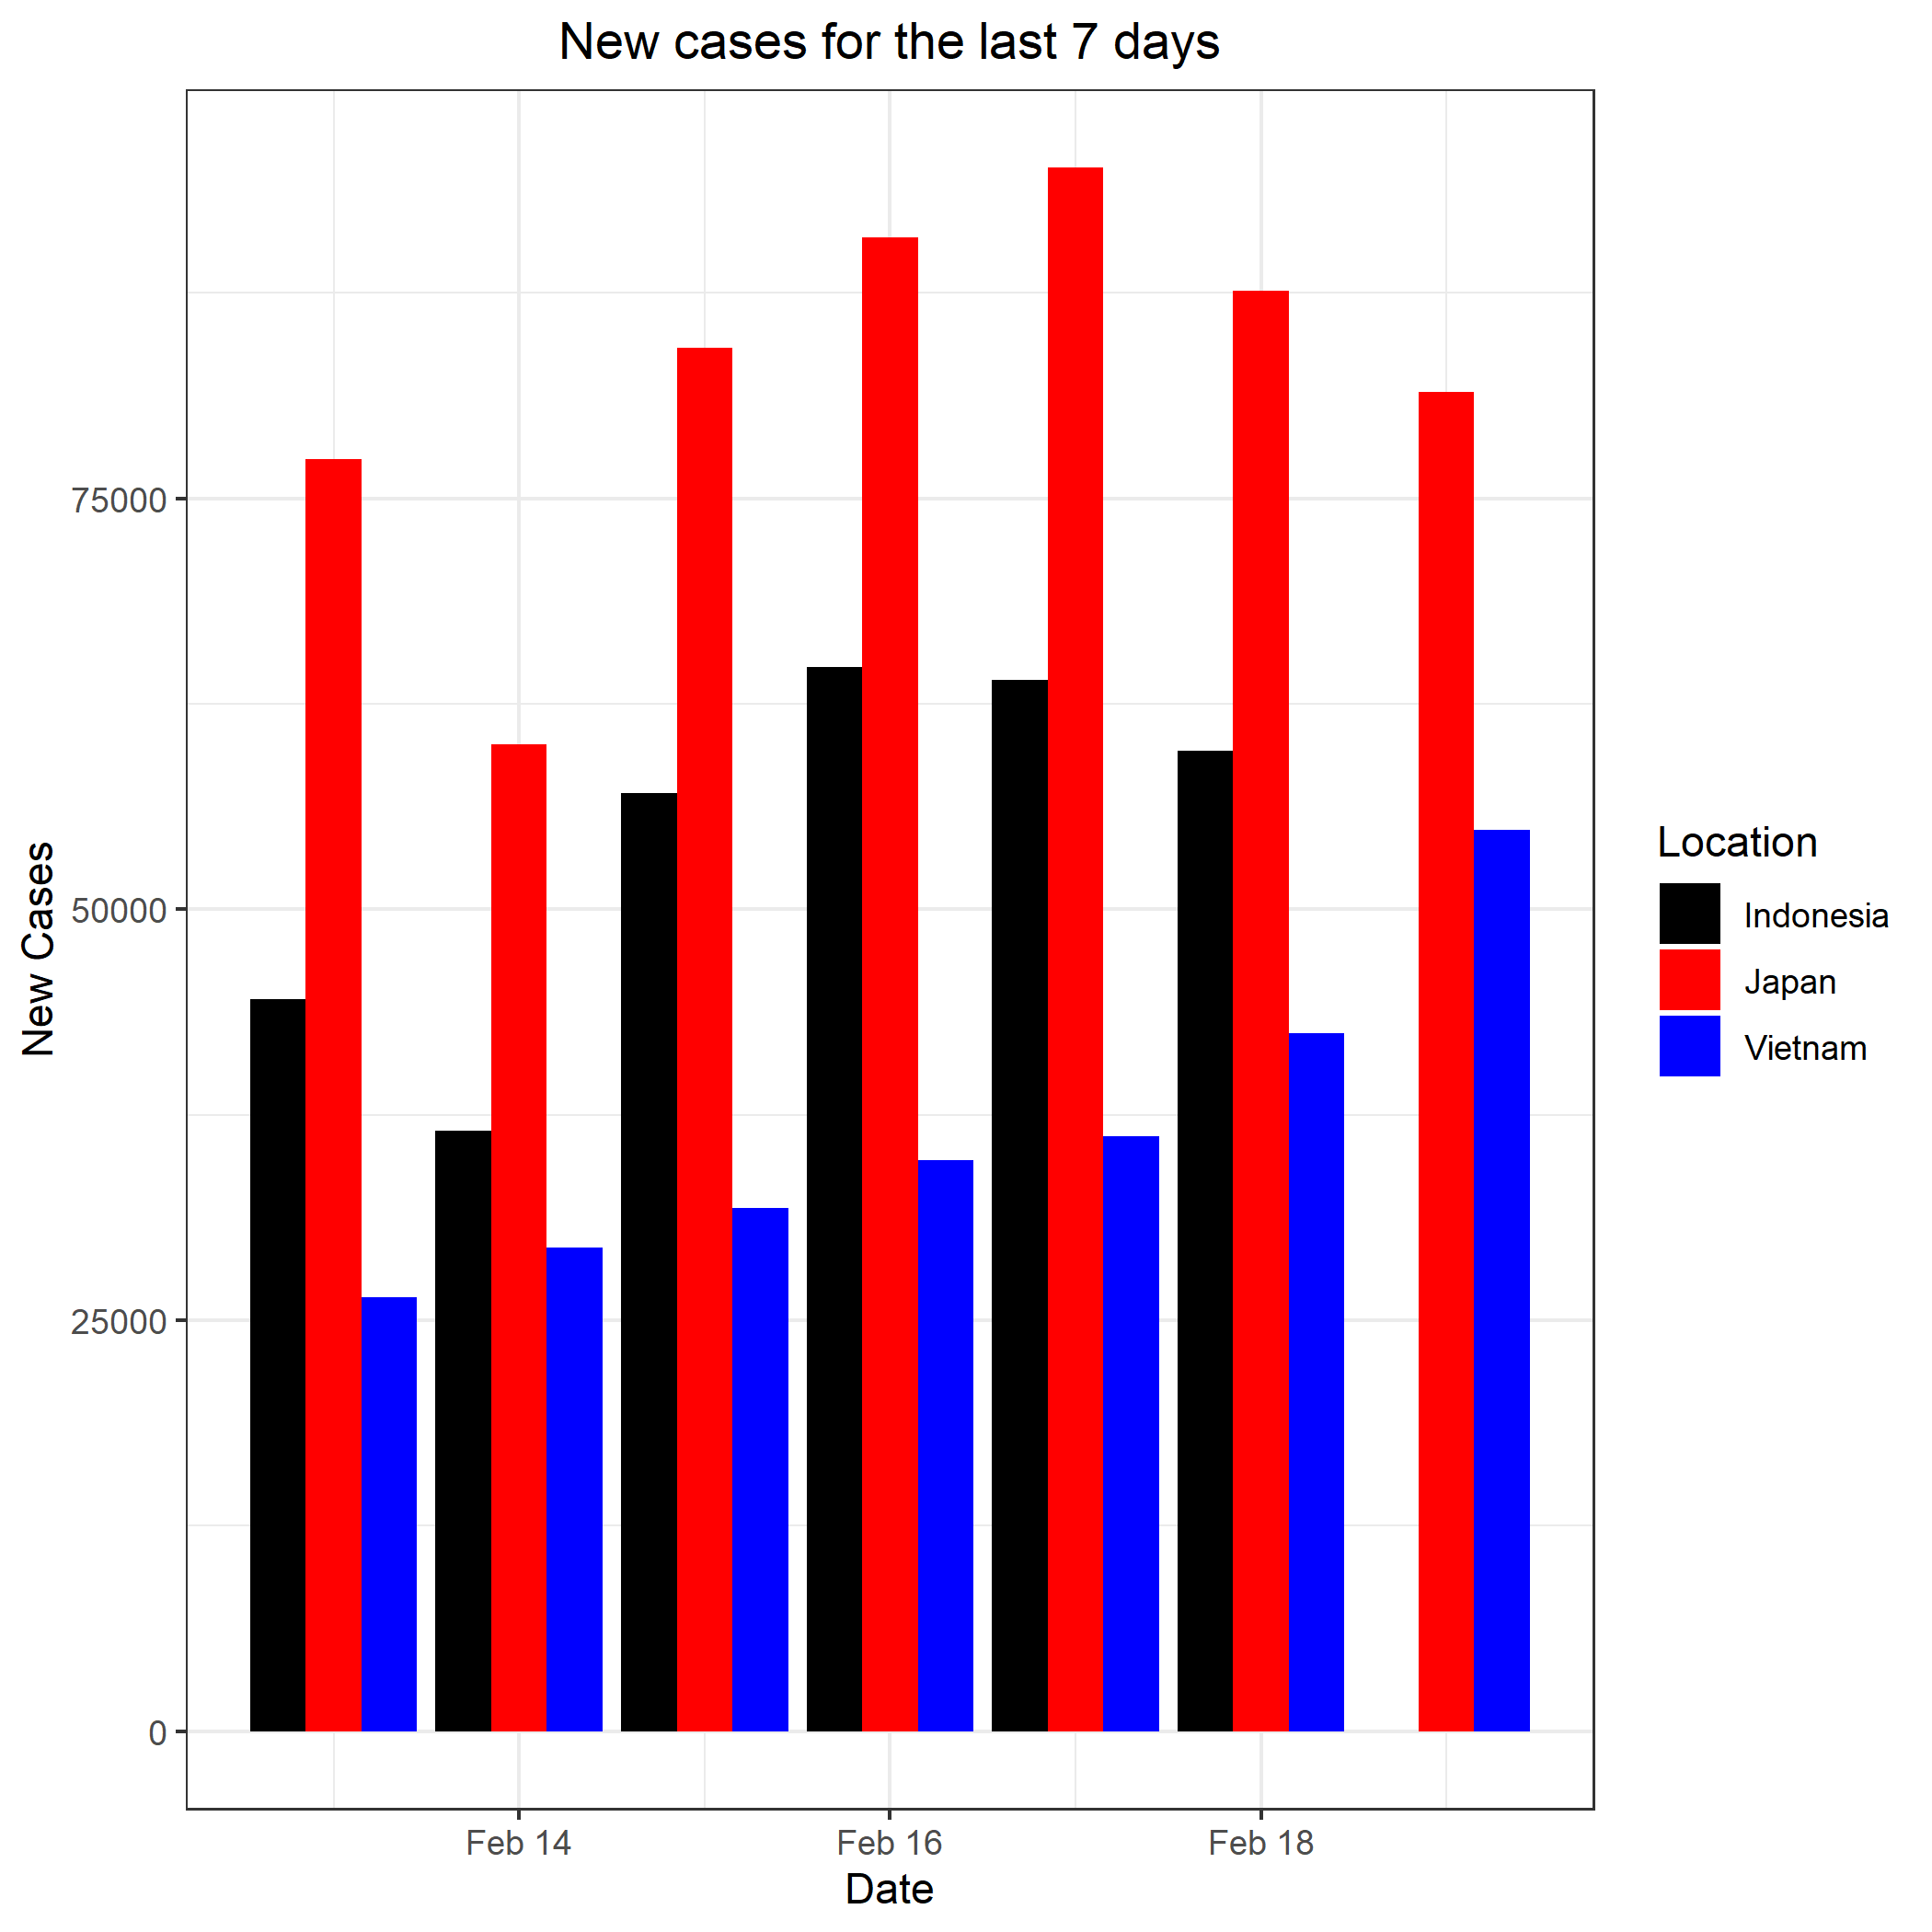
\includegraphics[scale=0.7]{iv/iv.3) New cases for the last 7 days.png}
        \end{center}
        \vspace{+3mm}\caption{\it Biểu đồ thể hiện nhiễm bệnh đã báo cáo của các quốc gia trong 7 ngày cuối của năm cuối cùng}
    \end{figure}
\item Vẽ biểu đồ thể hiện tử vong đã báo cáo của các quốc gia trong 7 ngày cuối của năm cuối cùng
\begin{lstlisting}
graph4 <- ggplot(data = thelastsevendays, aes(x = date, y = new_deaths,fill = factor(location))) +
  theme_bw() + geom_bar(stat = "identity", position = "dodge") +
  labs(title = "New deaths for the last 7 days", x = "Date", y = "New Deaths") +
  theme(plot.title = element_text(hjust = 0.5)) + scale_fill_manual("Location", values = c("Indonesia" = "black", "Japan" = "red", "Vietnam" = "blue"))

graph4
ggsave("iv.4) New deaths for the last 7 days.png", plot = graph4)
\end{lstlisting}
Kết quả
    \begin{figure}[H]
        \begin{center}
            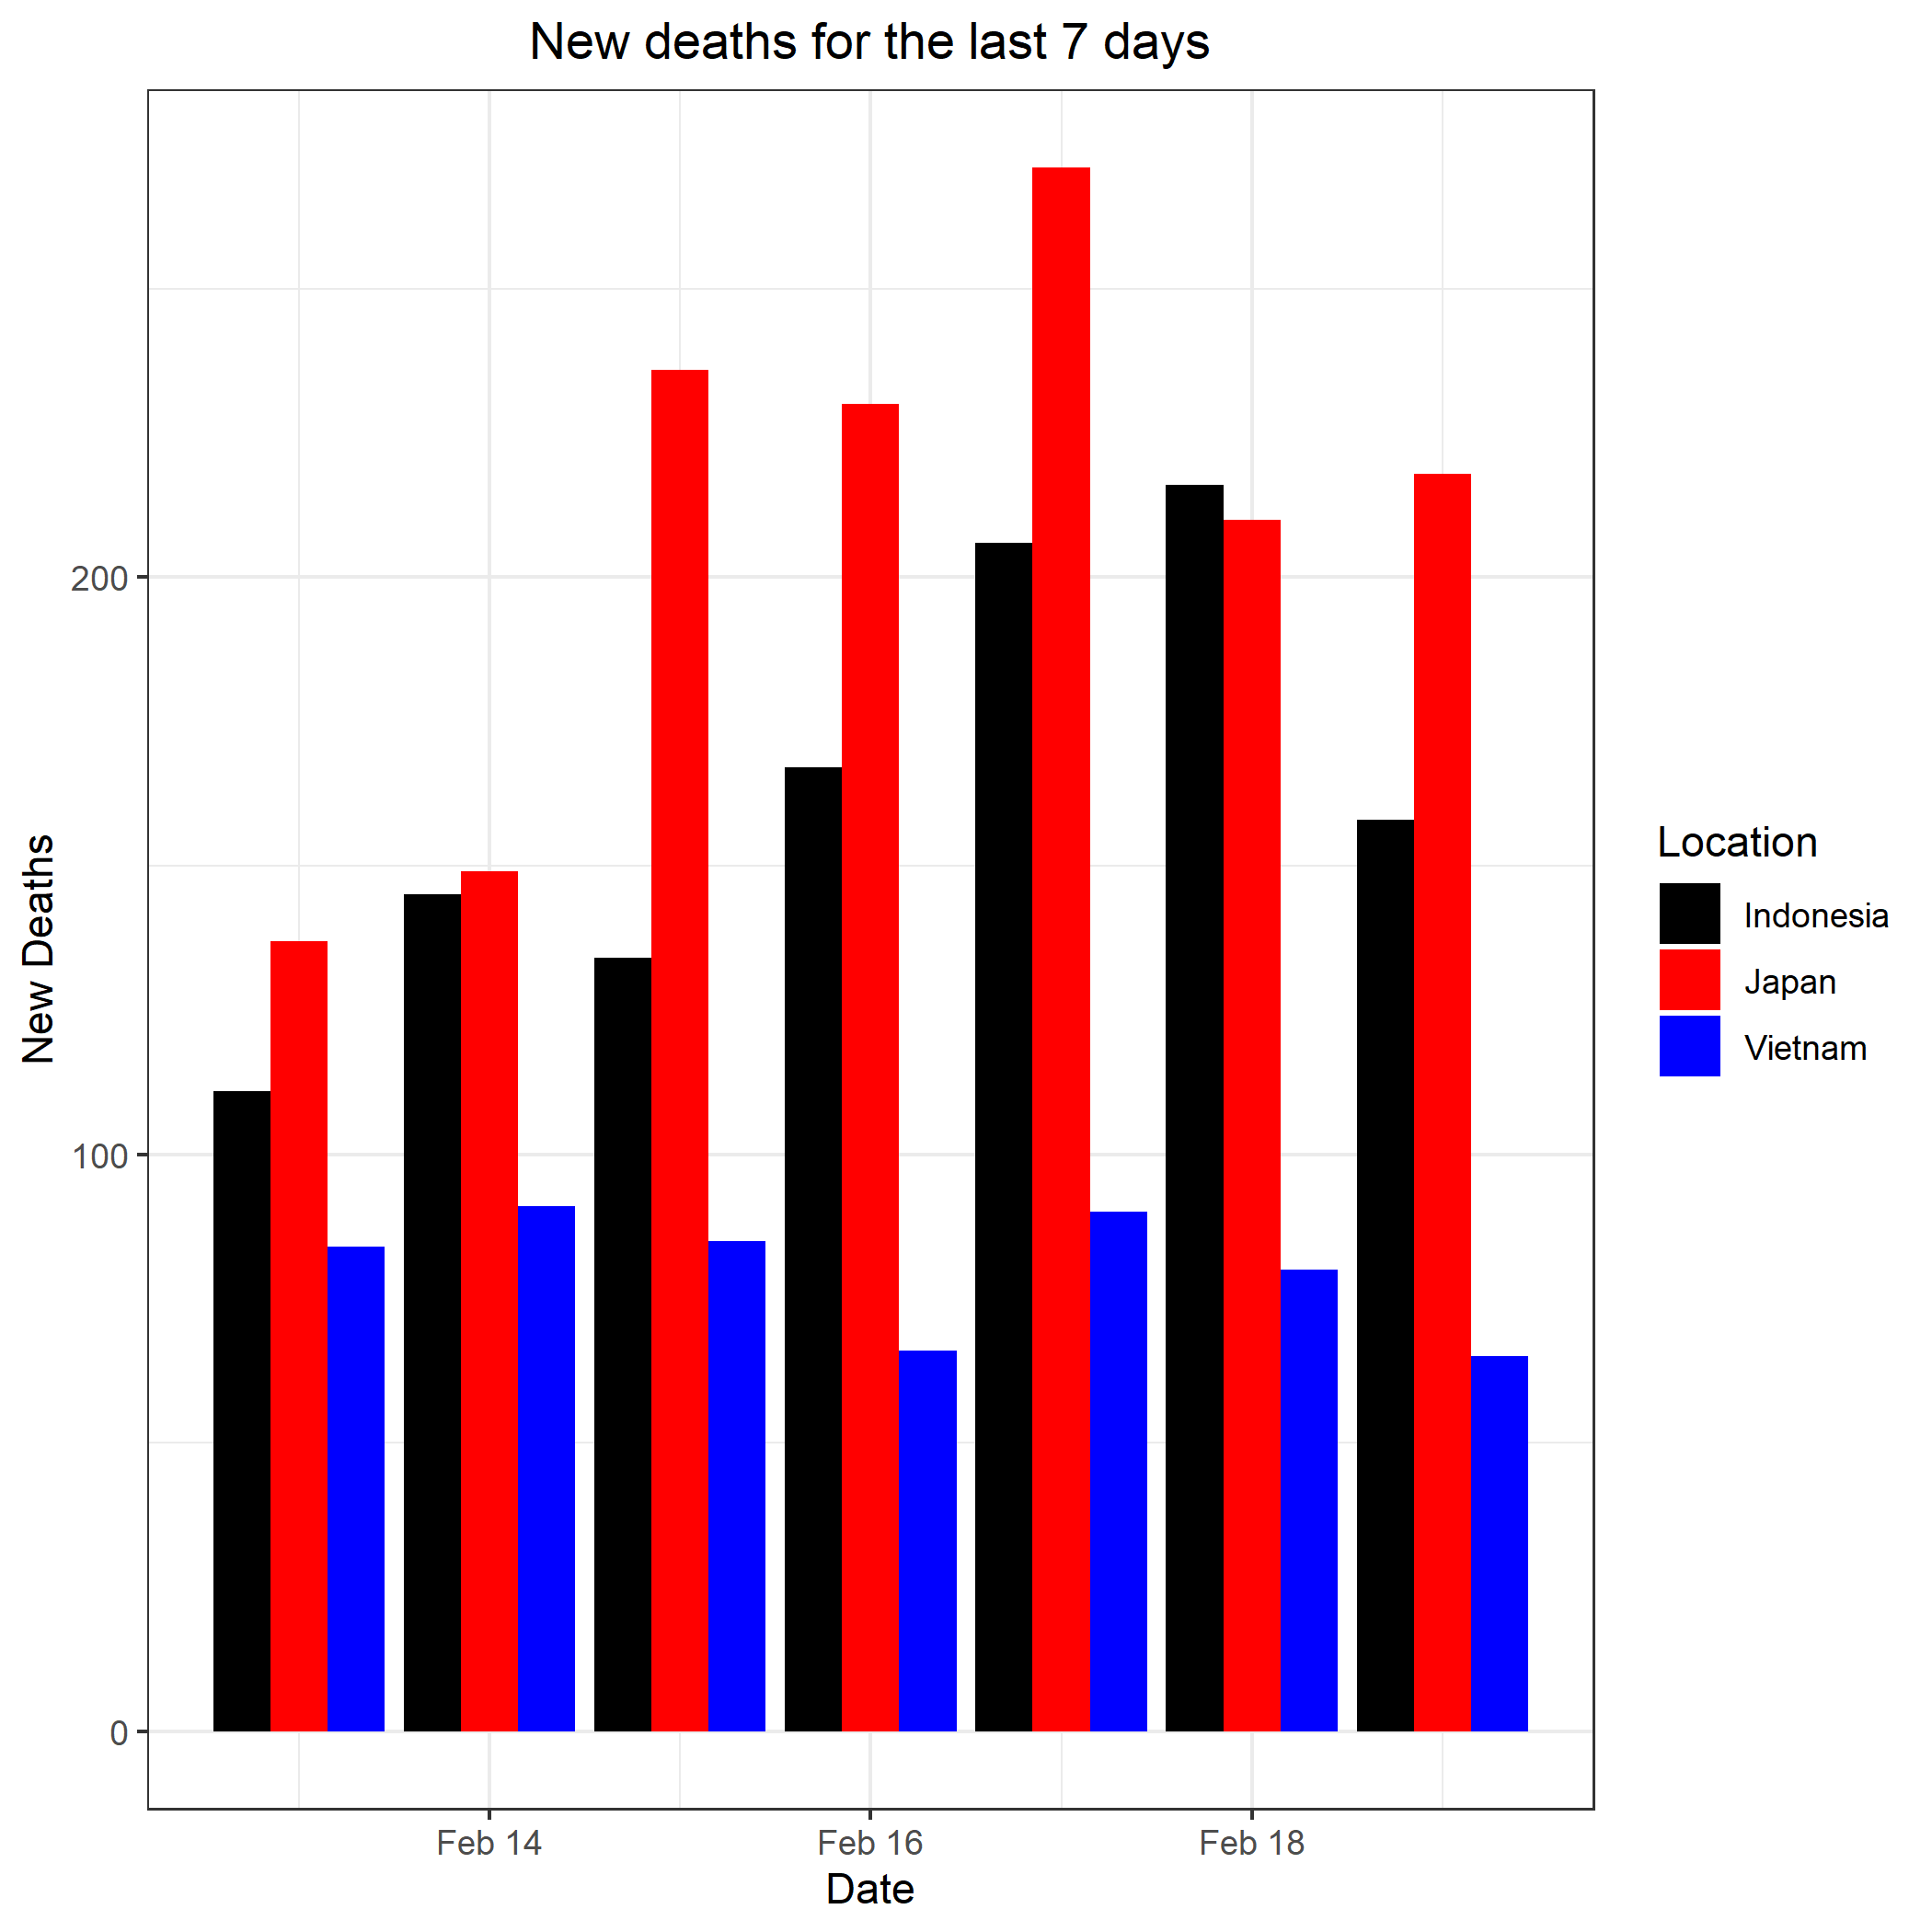
\includegraphics[scale=0.7]{iv/iv.4) New deaths for the last 7 days.png}
        \end{center}
        \vspace{+3mm}\caption{\it Biểu đồ thể hiện tử vong đã báo cáo của các quốc gia trong 7 ngày cuối của năm cuối cùng}
    \end{figure}
{\bf Xử lý chung cho câu 5 và 6} \\
Chúng ta lấy dữ liệu từ câu 5 phần $ii$ để làm cơ sở xử lý yêu cầu bài toán.
\begin{lstlisting}
datafromii.5 <- cbind(c("Indonesia","Japan","Vietnam"),as.data.frame(cases_outlier),as.data.frame(deaths_outlier))
colnames(datafromii.5) <- c("Country","casesOutliers","deathsOutliers")
\end{lstlisting}

\item Vẽ biểu đồ phổ đất nước xuất hiện outliers cho nhiễm bệnh
\begin{lstlisting}
graph5 <- ggplot(data = datafromii.5, aes(x=Country, y=casesOutliers, fill = factor(Country))) + 
  geom_bar(stat="identity") +
  theme_bw() +
  labs(title = "Number of infection outliers of each country") +
  theme(plot.title = element_text(hjust = 0.5)) + scale_fill_manual("Country", values = c("Indonesia" = "black", "Japan" = "red", "Vietnam" = "blue"))

graph5
ggsave("iv.5) caseOutPlot.png", plot = graph5)
\end{lstlisting}
Kết quả
    \begin{figure}[H]
        \begin{center}
            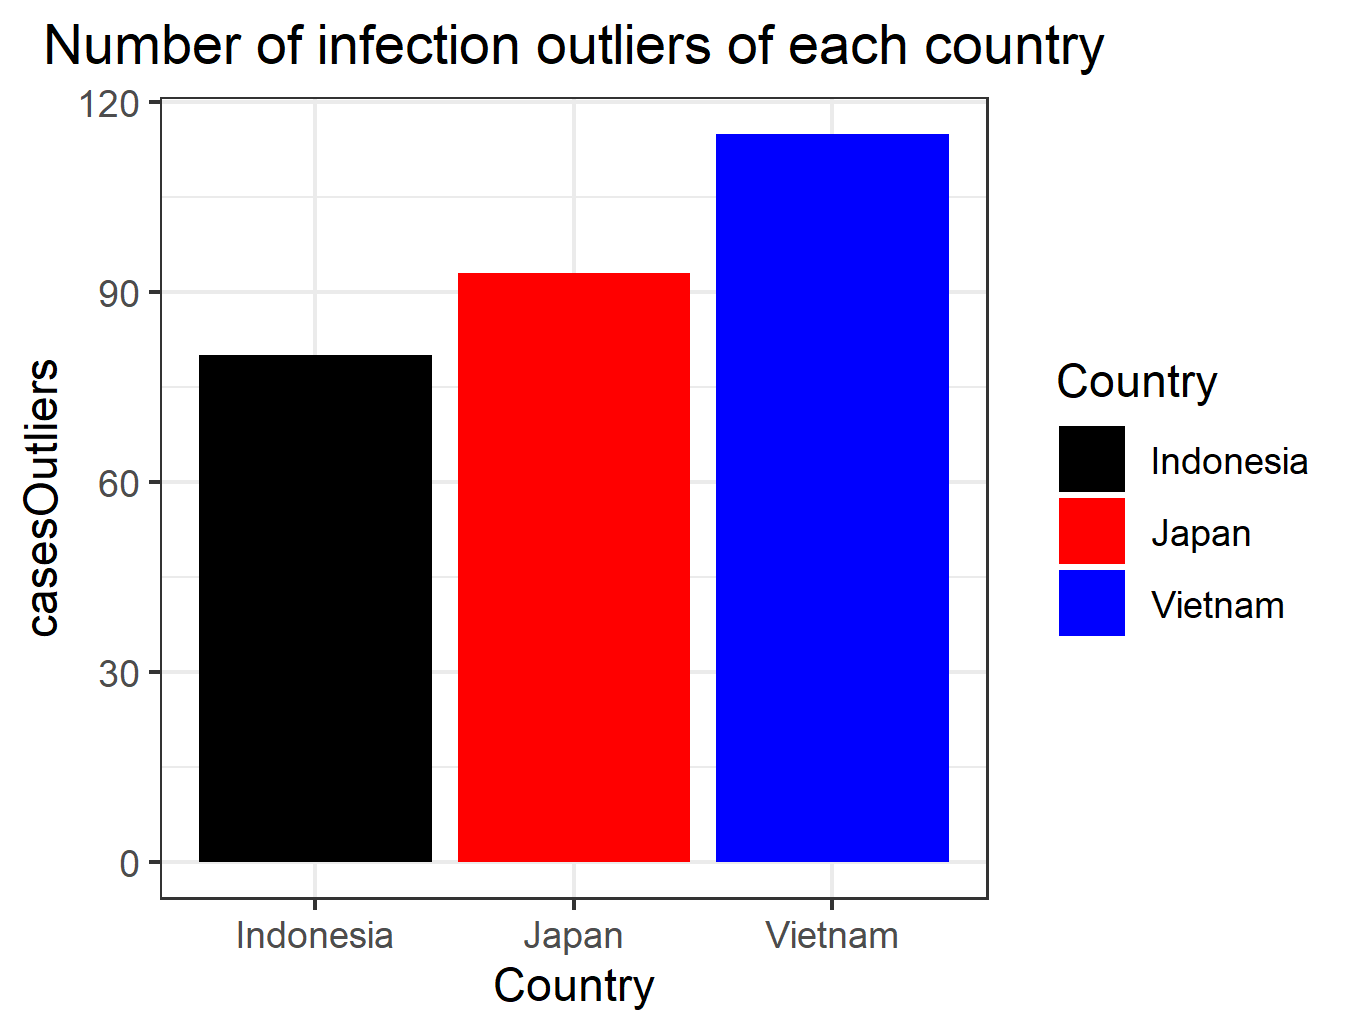
\includegraphics[scale=0.7]{iv/iv.5) caseOutPlot.png}
        \end{center}
        \vspace{+3mm}\caption{\it Biểu đồ phổ đất nước xuất hiện outliers cho nhiễm bệnh}
    \end{figure}
\item Vẽ biểu đồ phổ đất nước xuất hiện outliers cho tử vong
\begin{lstlisting}
graph6 <- ggplot(data = datafromii.5, aes(x=Country, y=deathsOutliers, fill = factor(Country))) + 
  geom_bar(stat="identity") +
  theme_bw() +
  labs(title = "Number of deaths outliers of each country") +
  theme(plot.title = element_text(hjust = 0.5)) + scale_fill_manual("Country", values = c("Indonesia" = "black", "Japan" = "red", "Vietnam" = "blue"))

graph6
ggsave("iv.6) deathOutPlot.png", plot = graph6)
\end{lstlisting}
Kết quả
    \begin{figure}[H]
        \begin{center}
            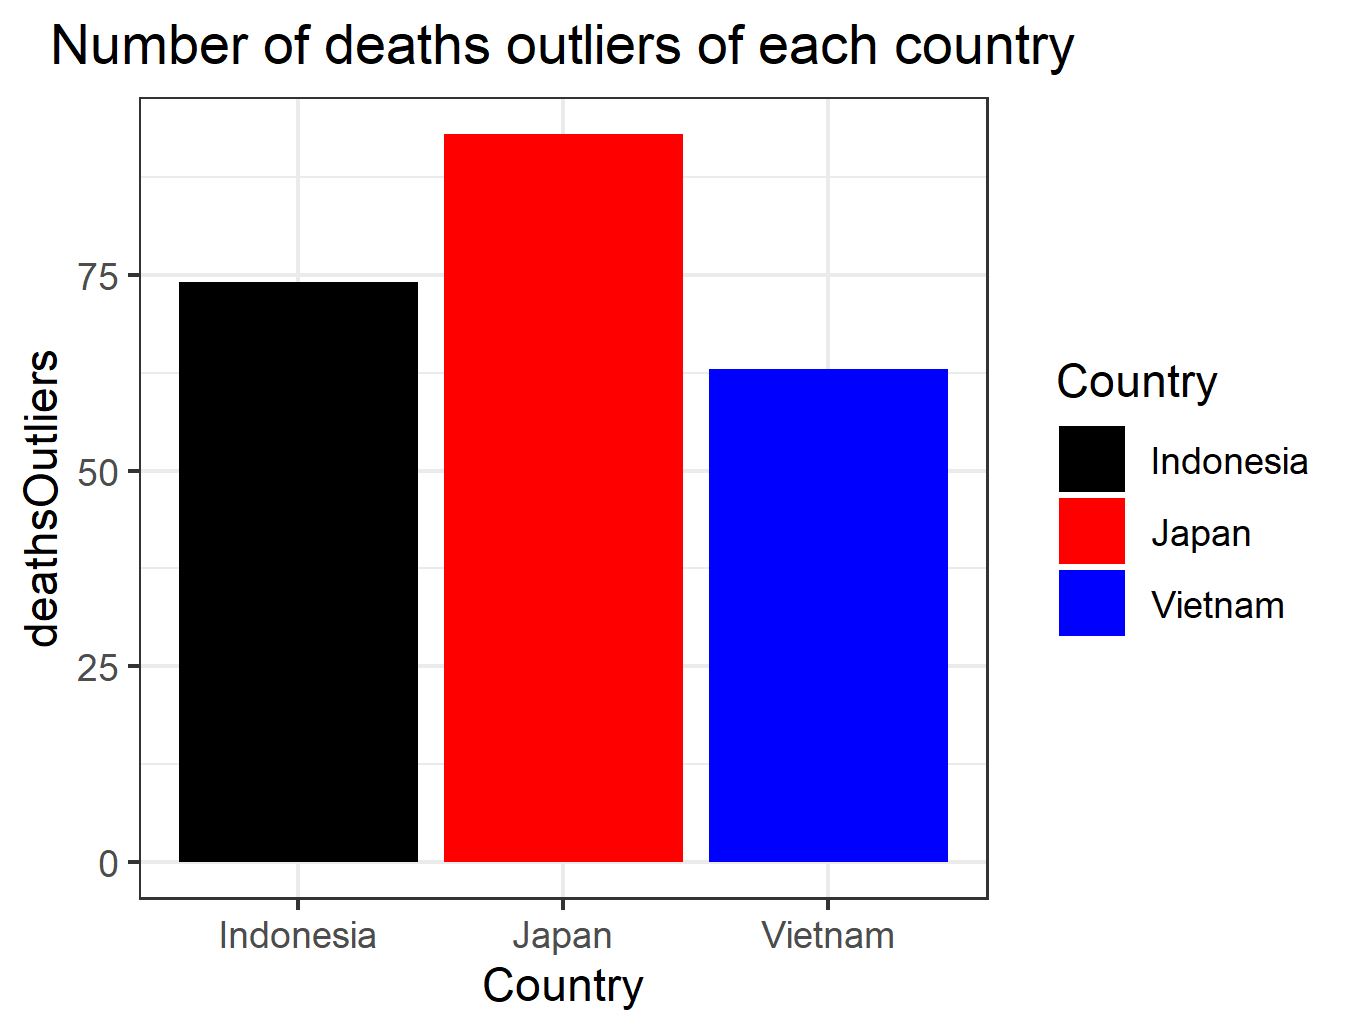
\includegraphics[scale=0.7]{iv/iv.6) deathOutPlot.png}
        \end{center}
        \vspace{+3mm}\caption{\it Biểu đồ đồ phổ đất nước xuất hiện outliers cho tử vong}
    \end{figure}
\end{enumerate}








\subsection{Nhiệm vụ v}
\begin{enumerate}[v)]
\item \textcolor{red}{Nhóm câu hỏi liên quan đến trực quan dữ liệu theo thời gian là tháng}
\end{enumerate}
Với mỗi quốc gia mà thuộc về nhóm, trên từng năm hãy vẽ biểu đồ thể hiện trục Ox là thời gian, trục Oy là nhiễm bệnh/tử vong. Hãy dùng 4 ký số của mã đề để vẽ 4 tháng tương ứng theo ký số đó. Nếu ký số là 0 thì lấy tháng là 10.

\textbf{Xử lí chung:} Đầu tiên chúng ta nhập dữ liệu vào bảng, sửa những giá trị âm lại thành giá trị dương, đồng thời định dạng ngày tháng lại để dễ dàng xử lí và sau đó lọc tiếp dữ liệu của từng nước cần được xử lí ra bảng.
\begin{lstlisting}
dataFile <- read_csv("owid-covid-data.csv", show_col_types = FALSE)
  
# convert negative entries to positive
dataFile$new_cases <- abs(dataFile$new_cases)
dataFile$new_deaths <- abs(dataFile$new_deaths)

# convert date to machine-readable format
dataFile$date <- as.Date(dataFile$date, format="%m/%d/%Y")
  
# separate country from database
dataFile_ISO <- subset(dataFile, iso_code==country_code)
\end{lstlisting}
Vì các câu hỏi như nhau đối với từng năm cần xử lí dữ liệu nên báo cáo chỉ giới thiệu qua cách xử lí đối với năm đầu tiên.
\begin{enumerate}[1)]
    \item Biểu đồ thể hiện thu thập dữ liệu nhiễm bệnh cho từng tháng\\
    Đầu tiên ta tách dữ liệu về các ca nhiễm bệnh của tất cả các tháng cần được xử lí ra bảng riêng, sau đó thêm một cột $month$ ứng với tên tháng cho từng ngày được báo cáo. Cuối cùng ta dùng $ggplot$ để vẽ đồ thị và $ggsave$ để lưu về máy.
    \begin{lstlisting}[gobble=4]
    dataFile_cases <- subset(dataFile_ISO, new_cases>0 &
                    ((format(date,"%m")=="01") | (format(date,"%m")=="03") |
                    (format(date,"%m")=="04") | (format(date,"%m")=="05")) & 
                    format(date,"%Y")=="2020",
                    select = c(date, new_cases))
    dataFile_cases <- dataFile_cases %>% mutate(month = as.numeric(format(dataFile_cases$date,"%m"))) %>%
                                       mutate(month = month.name[month])
    dataFile_cases$month = factor(dataFile_cases$month, levels = c("January", "March", "April", "May"))
    dataFile_cases_plot <- ggplot(data = dataFile_cases, mapping = aes(x = date, y = new_cases, label = new_cases)) +
                        geom_line() + geom_point() + 
                        facet_grid(~ dataFile_cases$month, scales = "free_x", drop = FALSE) +
                        labs(x = "",
                             y = "Number of new cases",
                             title = "New COVID-19 cases in Indonesia",
                             subtitle = "Number of newly reported COVID-19 cases by date in January, March, April and May of 2020") +
                        theme_bw() + theme(text = element_text(size = 14)) +
                        theme(plot.title = element_text(face = "bold")) +
                        theme(plot.subtitle = element_text(face = "italic")) +
                        theme(axis.text.x = element_text(angle = 0, size = 9)) +
                        theme(plot.margin = margin(1,1.2,0.5,1, "cm")) +
                        theme(panel.spacing.x = unit(4, "mm")) +
                        scale_y_continuous(labels = label_number())
    ggsave(dataFile_cases_plot, filename = paste(country_code,"2020_new_cases.pdf",sep="_"), width = 12, height = 6)
    \end{lstlisting}
    
    Kết quả
    
    \begin{figure}[H]
        \begin{center}
            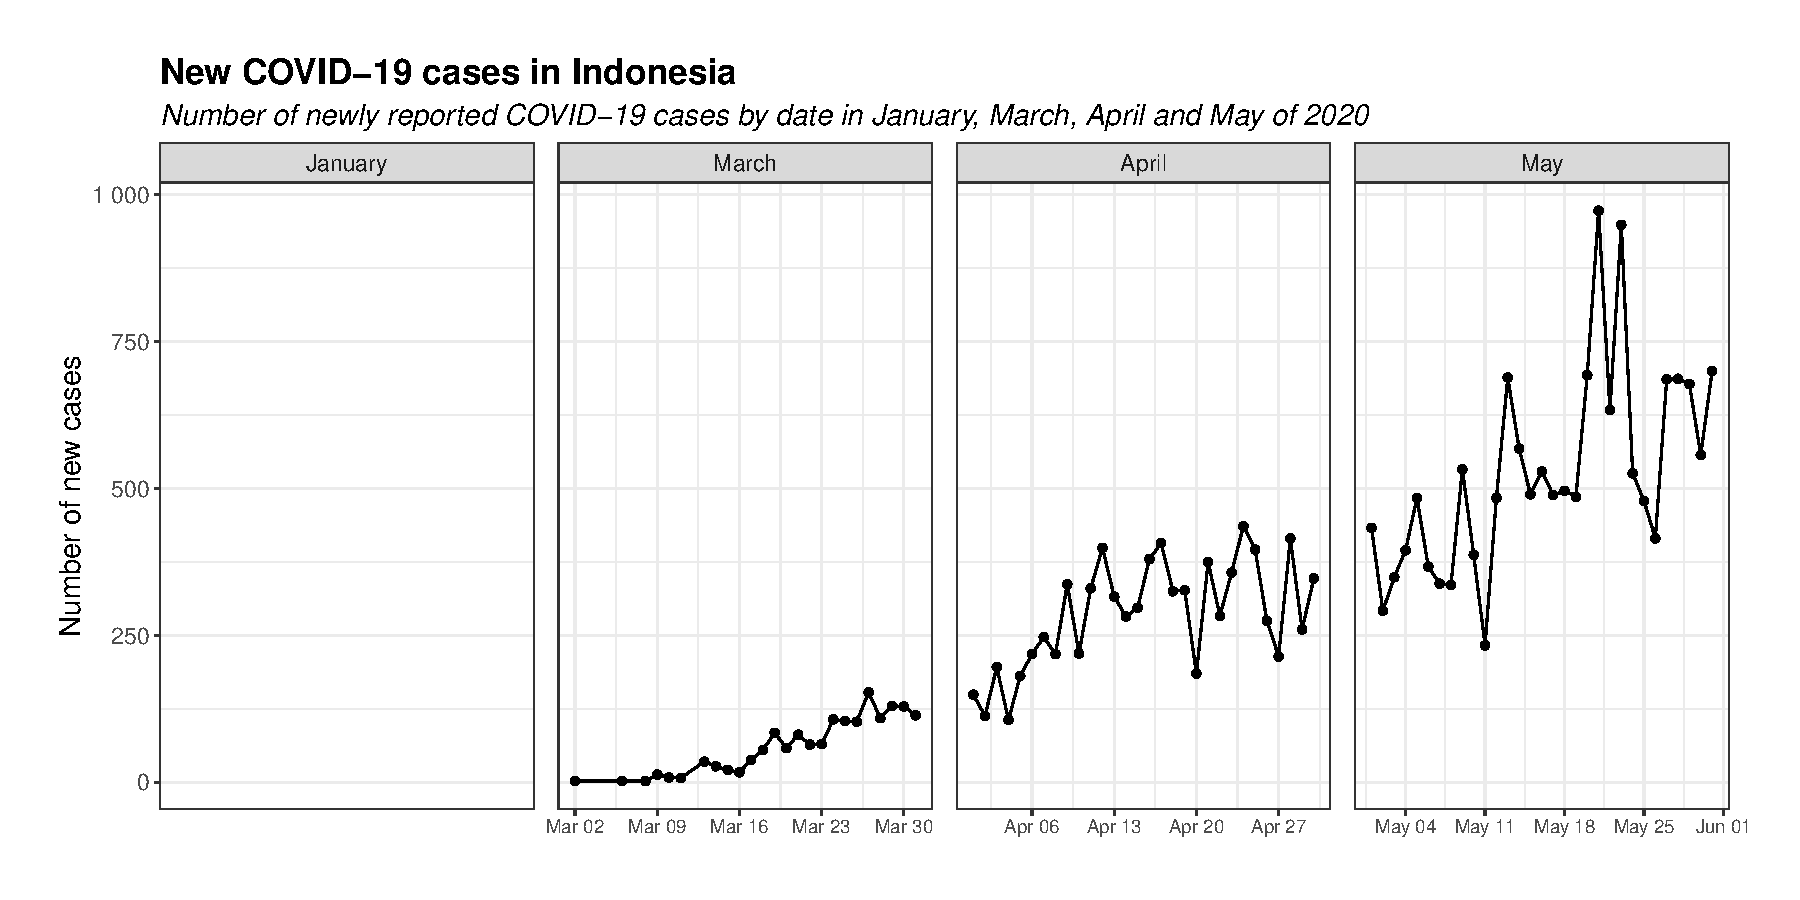
\includegraphics[scale=0.5]{v/IDN_2020_new_cases.pdf}
        \end{center}
    \caption{\it Biểu đồ thể hiện thu thập dữ liệu nhiễm bệnh cho từng tháng}
    \end{figure}
    \item Biểu đồ thể hiện thu thập dữ liệu tử vong cho từng tháng\\
    Tương tự câu 1), ta tách dữ liệu về các ca tử vong cho tất cả các tháng cần được xử lí.
    \begin{lstlisting}[gobble=4]
    dataFile_deaths <- subset(dataFile_ISO, new_deaths>0 &
                    ((format(date,"%m")=="01") | (format(date,"%m")=="03") |
                    (format(date,"%m")=="04") | (format(date,"%m")=="05")) & 
                    format(date,"%Y")=="2020",
                    select = c(date, new_deaths))
    dataFile_deaths <- dataFile_deaths %>% mutate(month = as.numeric(format(dataFile_deaths$date,"%m"))) %>%
                                       mutate(month = month.name[month])
    dataFile_deaths$month = factor(dataFile_deaths$month, levels = c("January", "March", "April", "May"))
    dataFile_deaths_plot <- ggplot(data = dataFile_deaths, mapping = aes(x = date, y = new_deaths, label = new_deaths)) +
                        geom_line() + geom_point() + 
                        facet_grid(~ dataFile_deaths$month, scales = "free_x", drop = FALSE) +
                        labs(x = "",
                             y = "Number of new deaths",
                             title = "New COVID-19 deaths in Indonesia",
                             subtitle = "Number of newly reported COVID-19 deaths by date in January, March, April and May of 2020") +
                        theme_bw() + theme(text = element_text(size = 14)) +
                        theme(plot.title = element_text(face = "bold")) +
                        theme(plot.subtitle = element_text(face = "italic")) +
                        theme(axis.text.x = element_text(angle = 0, size = 9)) +
                        theme(plot.margin = margin(1,1.2,0.5,1, "cm")) +
                        theme(panel.spacing.x = unit(4, "mm")) +
                        scale_y_continuous(labels = label_number())
    ggsave(dataFile_deaths_plot, filename =   paste(country_code,"2020_new_deaths.pdf",sep="_"), width = 12, height = 6)
    \end{lstlisting}
    
    Kết quả
    
    \begin{figure}[H]
        \begin{center}
            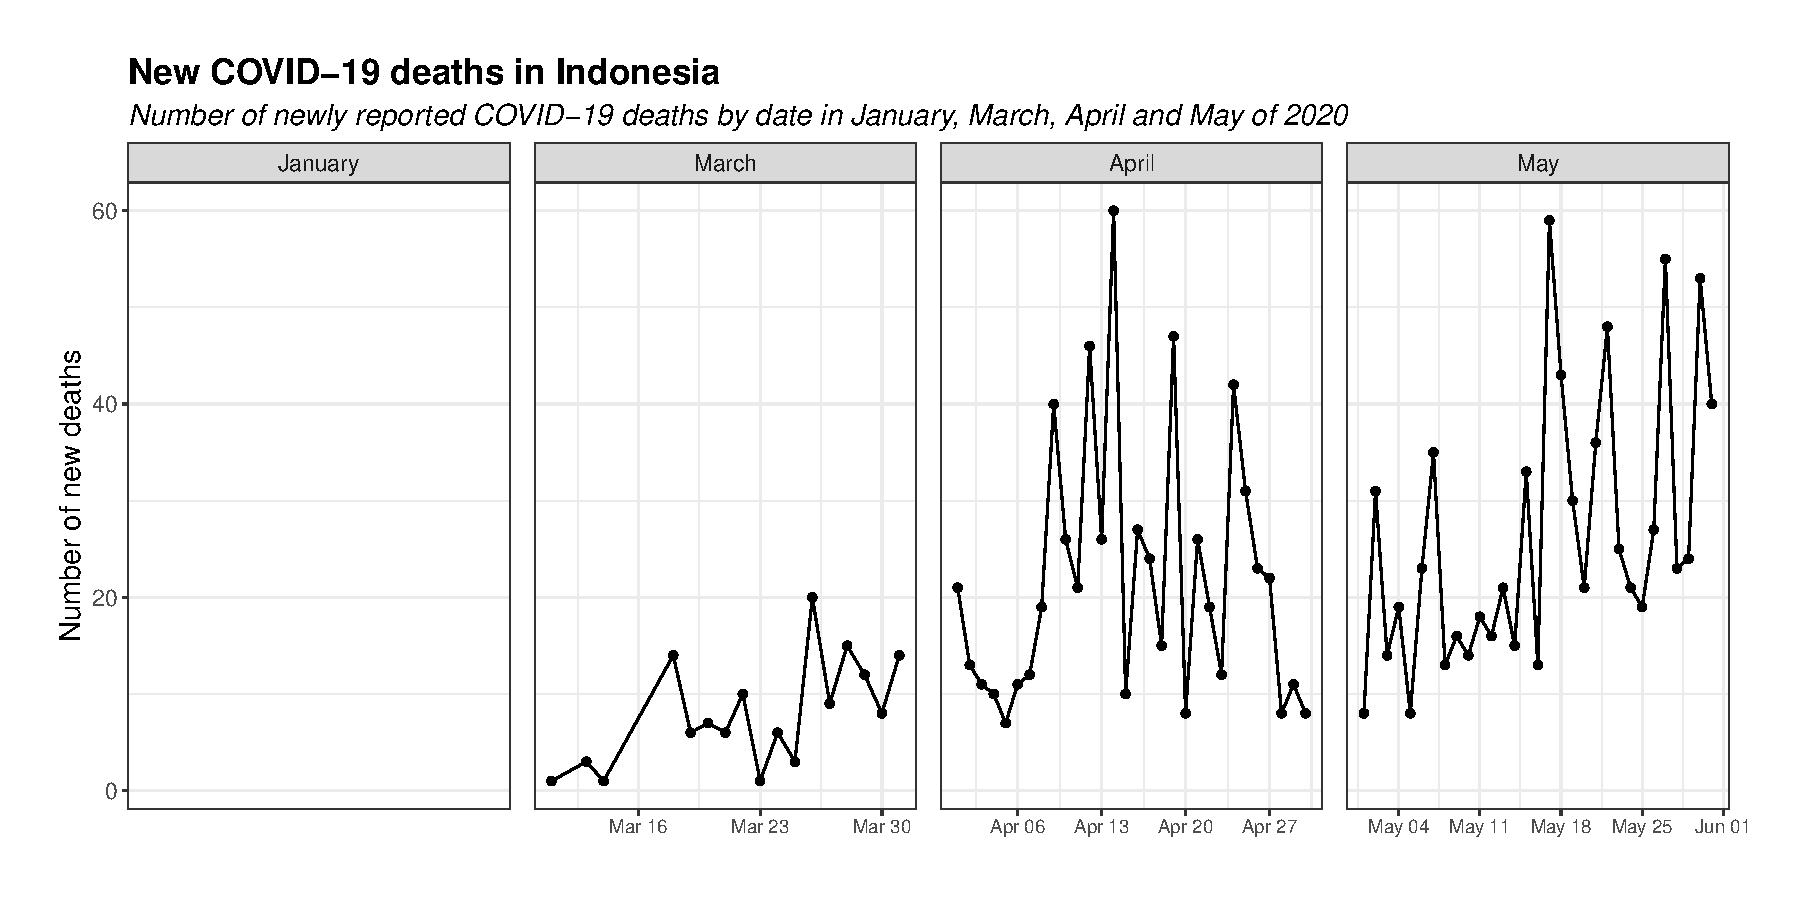
\includegraphics[scale=0.5]{v/IDN_2020_new_deaths.pdf}
        \end{center}
    \caption{\it Biểu đồ thể hiện thu thập dữ liệu tử vong cho từng tháng}
    \end{figure}
    \item Biểu đồ thể hiện thu thập dữ liệu gồm nhiễm bệnh và tử vong cho từng tháng \\
    Tương tự câu 2), ta tách dữ liệu về các ca nhiễm bệnh và tử vong cho tất cả các tháng cần được xử lí.
    \begin{lstlisting}[gobble=4]
    dataFile_cases <- subset(dataFile_ISO, new_cases>0 &
                    ((format(date,"%m")=="01") | (format(date,"%m")=="03") |
                    (format(date,"%m")=="04") | (format(date,"%m")=="05")) & 
                    format(date,"%Y")=="2020",
                    select = c(date, new_cases, new_deaths))
    dataFile_cases <- dataFile_cases %>% mutate(month = as.numeric(format(dataFile_cases$date,"%m"))) %>%
                                       mutate(month = month.name[month])
    dataFile_cases$month = factor(dataFile_cases$month, levels = c("January", "March", "April", "May"))
    dataFile_cases_plot <- ggplot(data = dataFile_cases, mapping = aes(x = date)) +
                        geom_line(aes(y = new_cases, color = "Cases")) + 
                        geom_line(aes(y = new_deaths, color = "Deaths")) + 
                        geom_point(aes(y = new_cases, color = "Cases")) +
                        geom_point(aes(y = new_deaths, color = "Deaths")) +
                        facet_grid(~ dataFile_cases$month, scales = "free_x", drop = FALSE) +
                        labs(x = "",
                             y = "Number of new cases",
                             title = "New COVID-19 cases (and deaths) in Indonesia",
                             subtitle = "Number of newly reported COVID-19 cases (and deaths) by date in January, March, April and May of 2020") +
                        scale_color_manual(values = colors) +
                        theme_bw() + theme(text = element_text(size = 14)) +
                        theme(plot.title = element_text(face = "bold")) +
                        theme(plot.subtitle = element_text(face = "italic")) +
                        theme(axis.text.x = element_text(angle = 0, size = 9)) +
                        theme(plot.margin = margin(1,1.2,0.5,1, "cm")) +
                        theme(panel.spacing.x = unit(4, "mm")) +
                        theme(legend.position = "bottom") +
                        theme(legend.title = element_blank()) +
                        scale_y_continuous(labels = label_number())
    ggsave(dataFile_cases_plot, filename = paste(country_code,"2020_new_cases_deaths.pdf",sep="_"), width = 12, height = 6)
    \end{lstlisting}
    
    Kết quả
    
    \begin{figure}[H]
        \begin{center}
            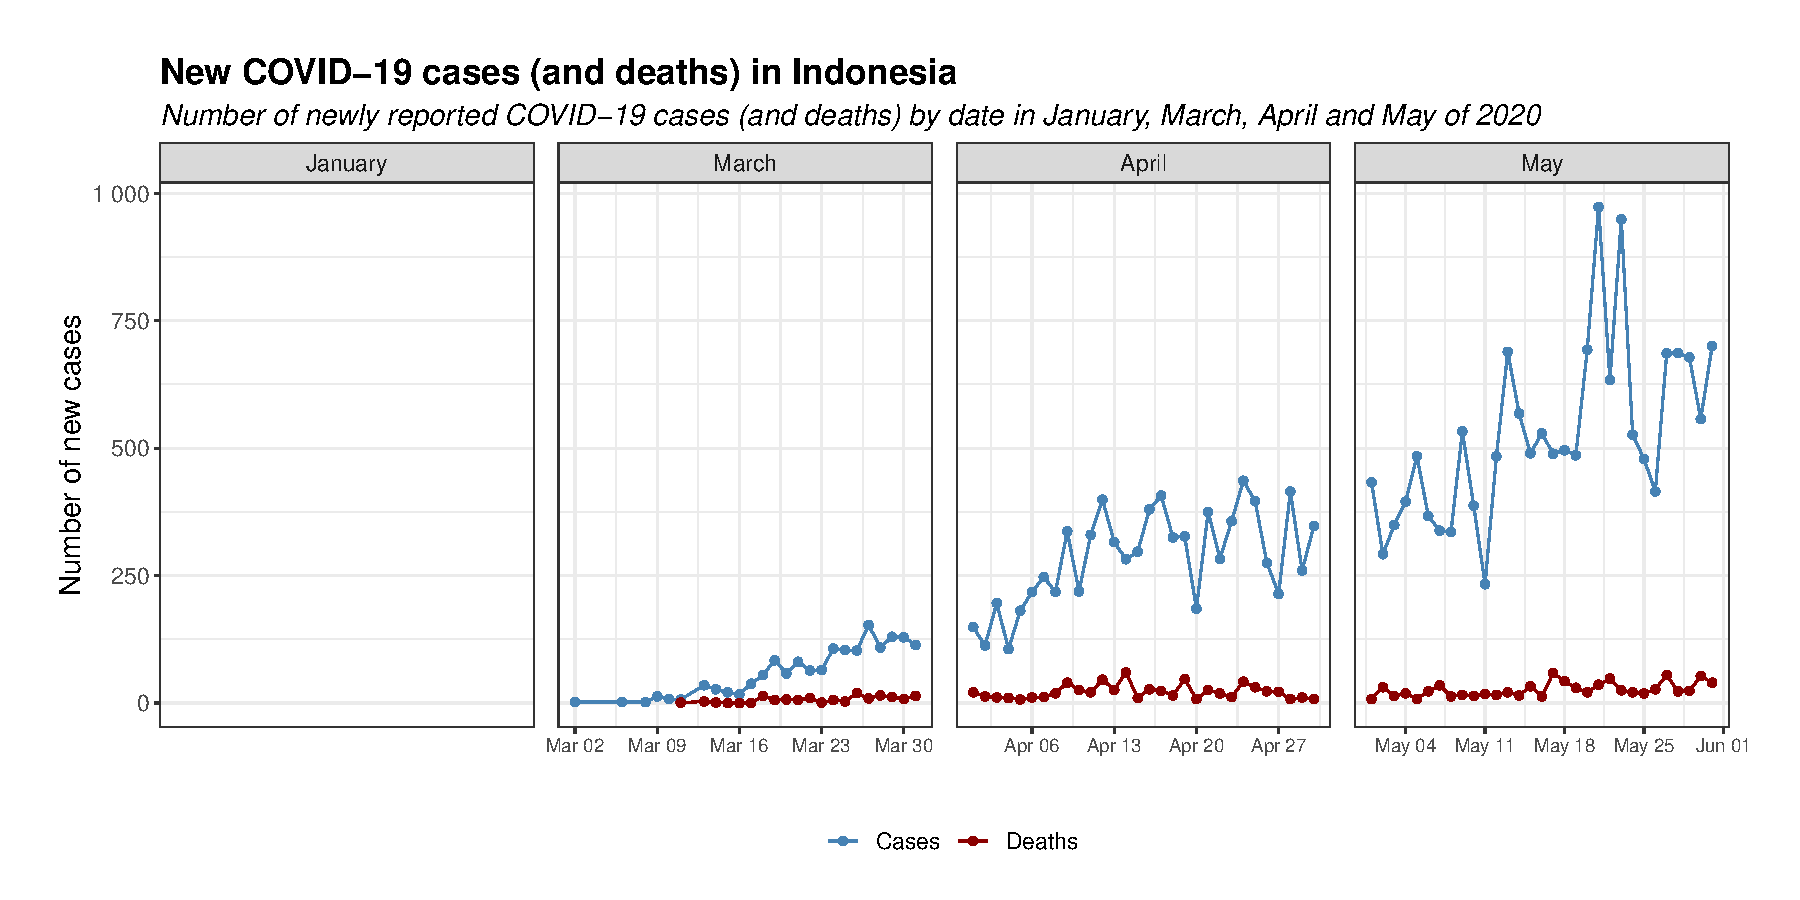
\includegraphics[scale=0.5]{v/IDN_2020_new_cases_deaths.pdf}
        \end{center}
    \caption{\it Biểu đồ thể hiện thu thập dữ liệu gồm nhiễm bệnh và tử vong cho từng tháng}
    \end{figure}
    \item Biểu đồ thể hiện thu thập dữ liệu nhiễm bệnh gồm 2 tháng cuối của năm\\
    Tương tự câu 1), ta tách dữ liệu về các ca nhiễm bệnh của 2 tháng cuối của năm.
    \begin{lstlisting}[gobble=4]
    dataFile_cases <- subset(dataFile_ISO, new_cases>0 &
                    ((format(date,"%m")=="11") | (format(date,"%m")=="12")) & 
                    format(date,"%Y")=="2020",
                    select = c(date, new_cases))
    dataFile_cases_plot <- ggplot(data = dataFile_cases, mapping = aes(x = date, y = new_cases, label = new_cases)) +
                        geom_line() + geom_point() + 
                        labs(x = "",
                             y = "Number of new cases",
                             title = "New COVID-19 cases in Indonesia",
                             subtitle = "Number of newly reported COVID-19 cases by date in November and December of 2020") +
                        theme_bw() + theme(text = element_text(size = 14)) +
                        theme(plot.title = element_text(face = "bold")) +
                        theme(plot.subtitle = element_text(face = "italic")) +
                        theme(axis.text.x = element_text(angle = 0, size = 9)) +
                        theme(plot.margin = margin(1,1.2,0.5,1, "cm")) +
                        theme(panel.spacing.x = unit(4, "mm")) +
                        scale_y_continuous(labels = label_number())
    ggsave(dataFile_cases_plot, filename = paste(country_code,"2020_new_cases_nov+dec.pdf",sep="_"), width = 12, height = 6)
    \end{lstlisting}
    
    Kết quả
    
    \begin{figure}[H]
        \begin{center}
            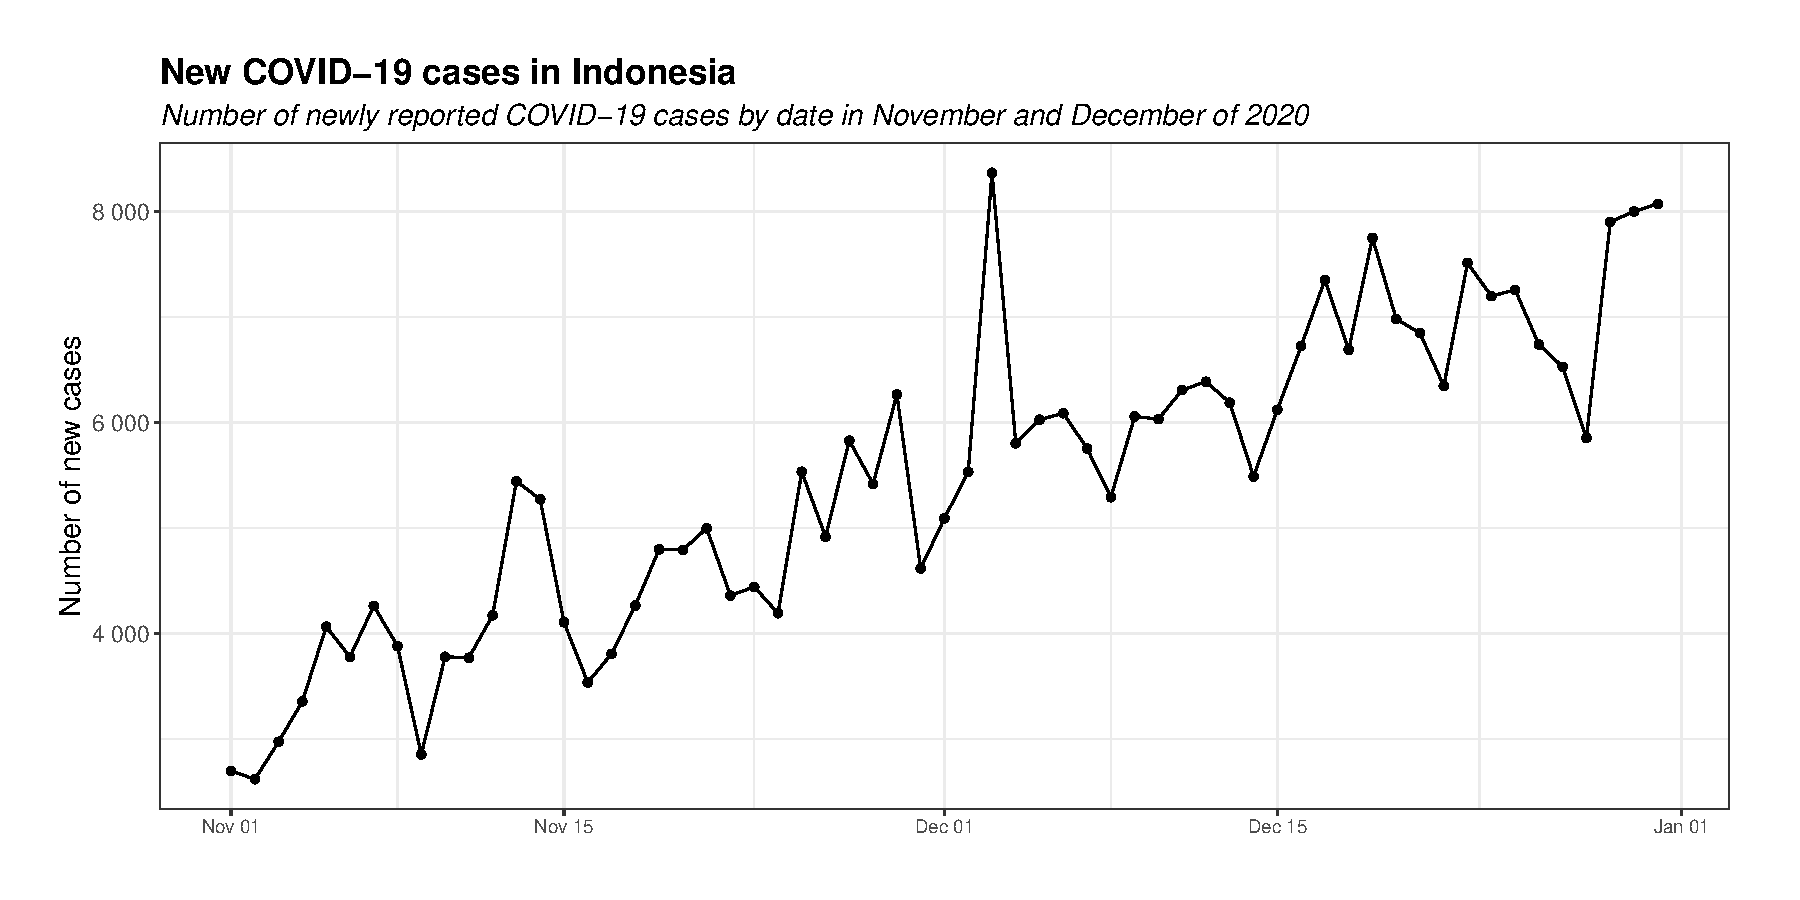
\includegraphics[scale=0.5]{v/IDN_2020_new_cases_nov+dec.pdf}
        \end{center}
    \caption{\it Biểu đồ thể hiện thu thập dữ liệu nhiễm bệnh gồm 2 tháng cuối của năm}
    \end{figure}
    \item Biểu đồ thể hiện thu thập dữ liệu tử vong gồm 2 tháng cuối của năm\\
    Tương tự câu 2), ta tách dữ liệu về các ca tử vong của 2 tháng cuối của năm.
    \begin{lstlisting}[gobble=4]
    dataFile_deaths <- subset(dataFile_ISO, new_deaths>0 &
                    ((format(date,"%m")=="11") | (format(date,"%m")=="12")) & 
                    format(date,"%Y")=="2020",
                    select = c(date, new_deaths))
    dataFile_deaths_plot <- ggplot(data = dataFile_deaths, mapping = aes(x = date, y = new_deaths, label = new_deaths)) +
                        geom_line() + geom_point() + 
                        labs(x = "",
                             y = "Number of new deaths",
                             title = "New COVID-19 deaths in Indonesia",
                             subtitle = "Number of newly reported COVID-19 deaths by date in November and December of 2020") +
                        theme_bw() + theme(text = element_text(size = 14)) +
                        theme(plot.title = element_text(face = "bold")) +
                        theme(plot.subtitle = element_text(face = "italic")) +
                        theme(axis.text.x = element_text(angle = 0, size = 9)) +
                        theme(plot.margin = margin(1,1.2,0.5,1, "cm")) +
                        theme(panel.spacing.x = unit(4, "mm")) +
                        scale_y_continuous(labels = label_number())
    ggsave(dataFile_deaths_plot, filename = paste(country_code,"2020_new_deaths_nov+dec.pdf",sep="_"), width = 12, height = 6)
    \end{lstlisting}
    
    Kết quả
    
    \begin{figure}[H]
        \begin{center}
            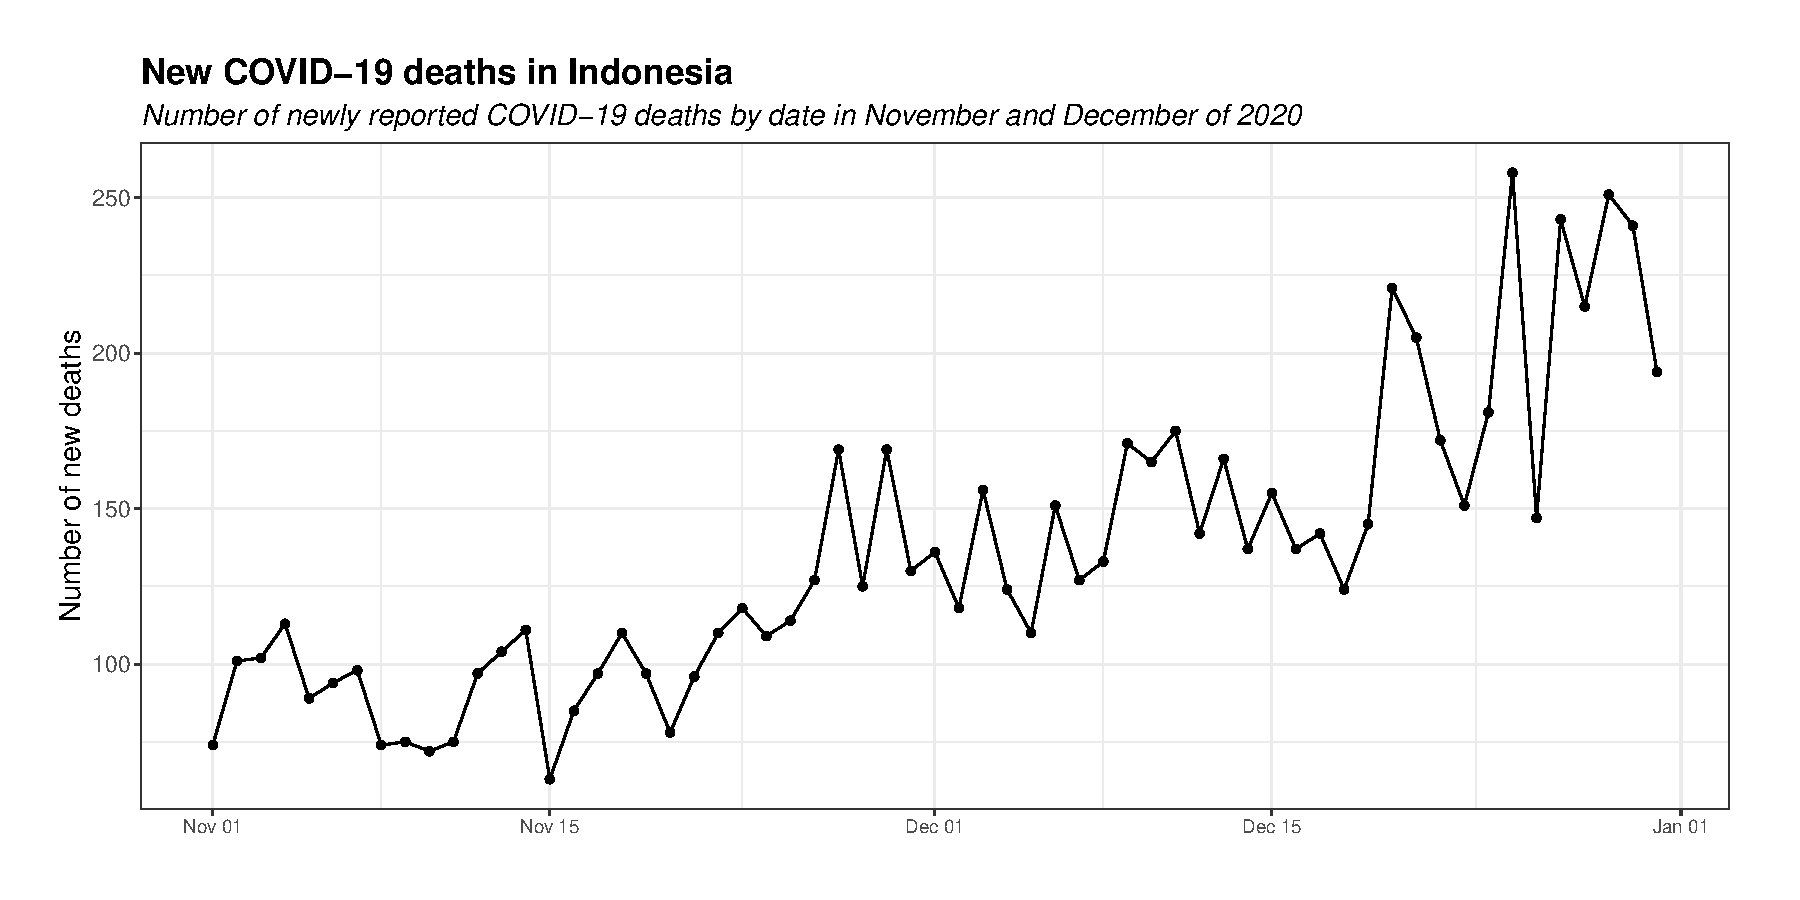
\includegraphics[scale=0.5]{v/IDN_2020_new_deaths_nov+dec.pdf}
        \end{center}
    \caption{\it Biểu đồ thể hiện thu thập dữ liệu tử vong gồm 2 tháng cuối của năm}
    \end{figure}
    \item Biểu đồ thể hiện thu thập dữ liệu gồm nhiễm bệnh và tử vong gồm 2 tháng cuối của năm\\
    Tương tự câu 3), ta tách dữ liệu về các ca nhiễm bệnh và tử vong cho 2 tháng cuối của năm.
    \begin{lstlisting}[gobble=4]
    dataFile_cases <- subset(dataFile_ISO, new_cases>0 &
                    ((format(date,"%m")=="11") | (format(date,"%m")=="12")) & 
                    format(date,"%Y")=="2020",
                    select = c(date, new_cases, new_deaths))
    dataFile_cases_plot <- ggplot(data = dataFile_cases, mapping = aes(x = date)) +
                        geom_line(aes(y = new_cases, color = "Cases")) + 
                        geom_line(aes(y = new_deaths, color = "Deaths")) + 
                        geom_point(aes(y = new_cases, color = "Cases")) +
                        geom_point(aes(y = new_deaths, color = "Deaths")) +
                        labs(x = "",
                             y = "Number of new cases",
                             title = "New COVID-19 cases (and deaths) in Indonesia",
                             subtitle = "Number of newly reported COVID-19 cases (and deaths) by date in November and December of 2020") +
                        scale_color_manual(values = colors) +
                        theme_bw() + theme(text = element_text(size = 14)) +
                        theme(plot.title = element_text(face = "bold")) +
                        theme(plot.subtitle = element_text(face = "italic")) +
                        theme(axis.text.x = element_text(angle = 0, size = 9)) +
                        theme(plot.margin = margin(1,1.2,0.5,1, "cm")) +
                        theme(panel.spacing.x = unit(4, "mm")) +
                        theme(legend.position = "bottom") +
                        theme(legend.title = element_blank()) +
                        scale_y_continuous(labels = label_number())
    ggsave(dataFile_cases_plot, filename = paste(country_code,"2020_new_cases_deaths_nov+dec.pdf",sep="_"), width = 12, height = 6)
    \end{lstlisting}
    
    Kết quả
    
    \begin{figure}[H]
        \begin{center}
            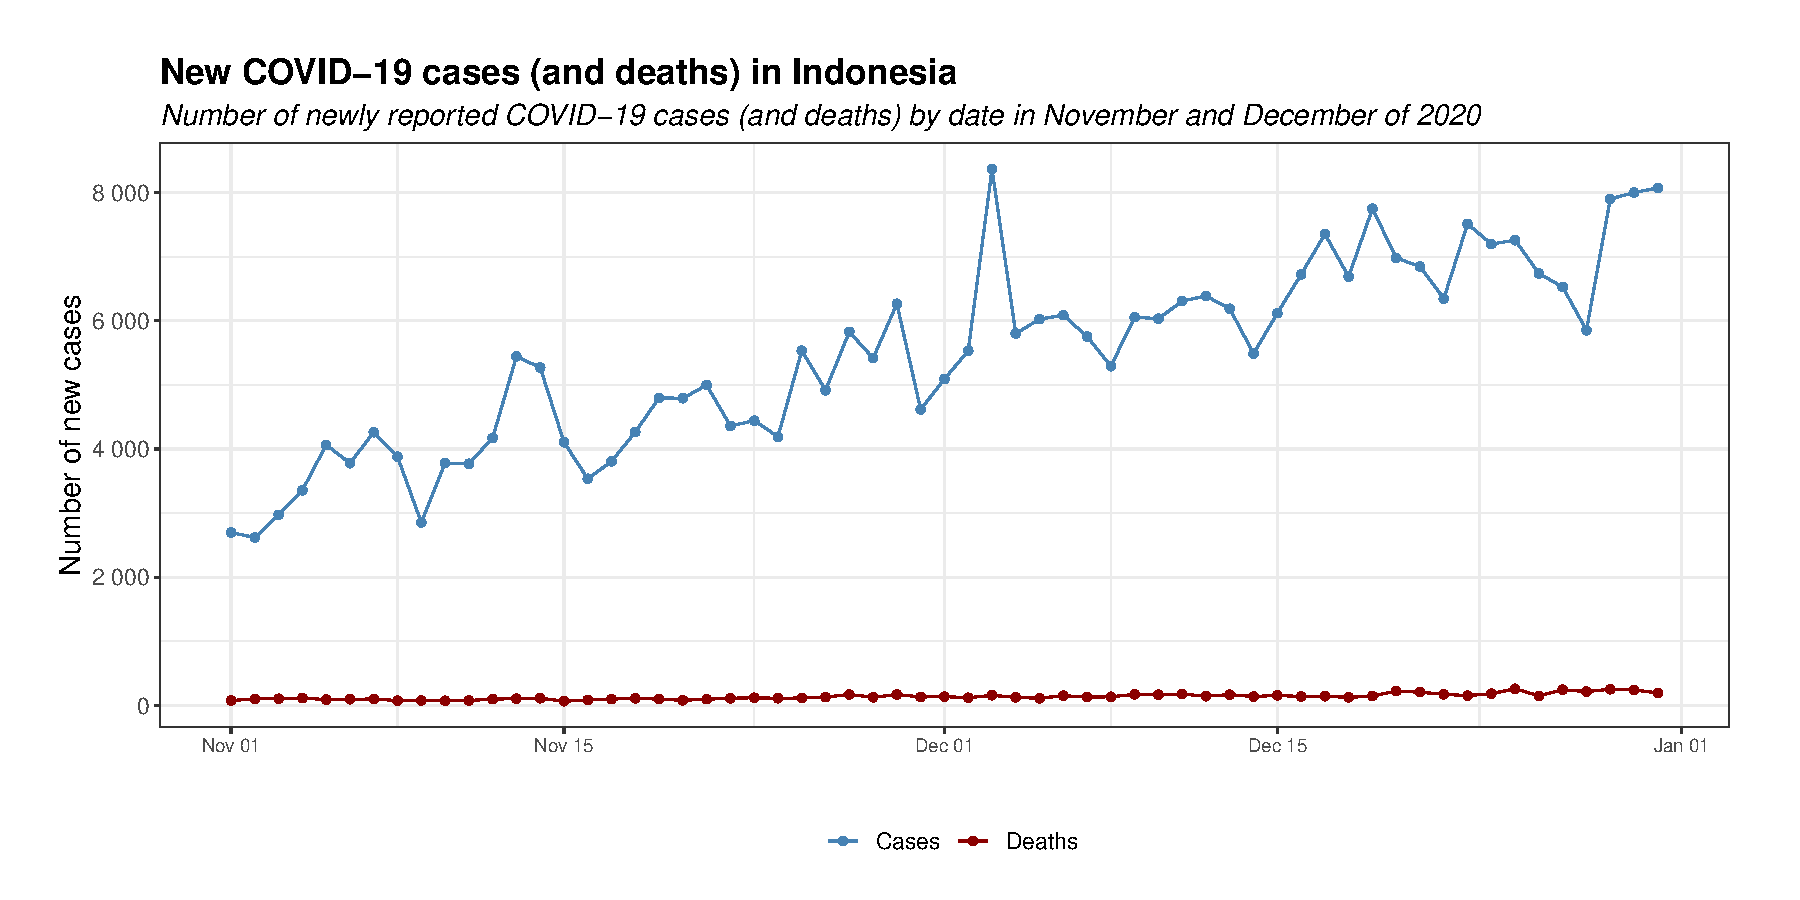
\includegraphics[scale=0.5]{v/IDN_2020_new_cases_deaths_nov+dec.pdf}
        \end{center}
    \caption{\it Biểu đồ thể hiện thu thập dữ liệu gồm nhiễm bệnh và tử vong gồm 2 tháng cuối của năm}
    \end{figure}
    \item Biểu đồ thể hiện thu thập dữ liệu nhiễm bệnh tích lũy cho từng tháng\\
    Tương tự câu 1), sau đó ta tiến hành cộng tích luỹ số ca nhiễm với nhau bằng $cumsum$
    \begin{lstlisting}[gobble=4]
    dataFile_cases <- subset(dataFile_ISO, new_cases>0 &
                    ((format(date,"%m")=="01") | (format(date,"%m")=="03") |
                    (format(date,"%m")=="04") | (format(date,"%m")=="05")) & 
                    format(date,"%Y")=="2020",
                    select = c(date, new_cases))
    dataFile_cases$new_cases <- cumsum(dataFile_cases$new_cases)
    dataFile_cases <- dataFile_cases %>% mutate(month = as.numeric(format(dataFile_cases$date,"%m"))) %>%
                                       mutate(month = month.name[month])
    dataFile_cases$month = factor(dataFile_cases$month, levels = c("January", "March", "April", "May"))
    dataFile_cases_plot <- ggplot(data = dataFile_cases, mapping = aes(x = date, y = new_cases, label = new_cases)) +
                        geom_line() + geom_point() + 
                        facet_grid(~ dataFile_cases$month, scales = "free_x", drop = FALSE) +
                        labs(x = "",
                             y = "Number of cases",
                             title = "COVID-19 cases in Indonesia",
                             subtitle = "Number of cumulative COVID-19 cases by date in January, March, April and May of 2020") +
                        theme_bw() + theme(text = element_text(size = 14)) +
                        theme(plot.title = element_text(face = "bold")) +
                        theme(plot.subtitle = element_text(face = "italic")) +
                        theme(axis.text.x = element_text(angle = 0, size = 9)) +
                        theme(plot.margin = margin(1,1.2,0.5,1, "cm")) +
                        theme(panel.spacing.x = unit(4, "mm")) +
                        scale_y_continuous(labels = label_number())
    ggsave(dataFile_cases_plot, filename = paste(country_code,"2020_cumulative_cases.pdf",sep="_"), width = 12, height = 6)
    \end{lstlisting}
    Kết quả
    
    \begin{figure}[H]
        \begin{center}
            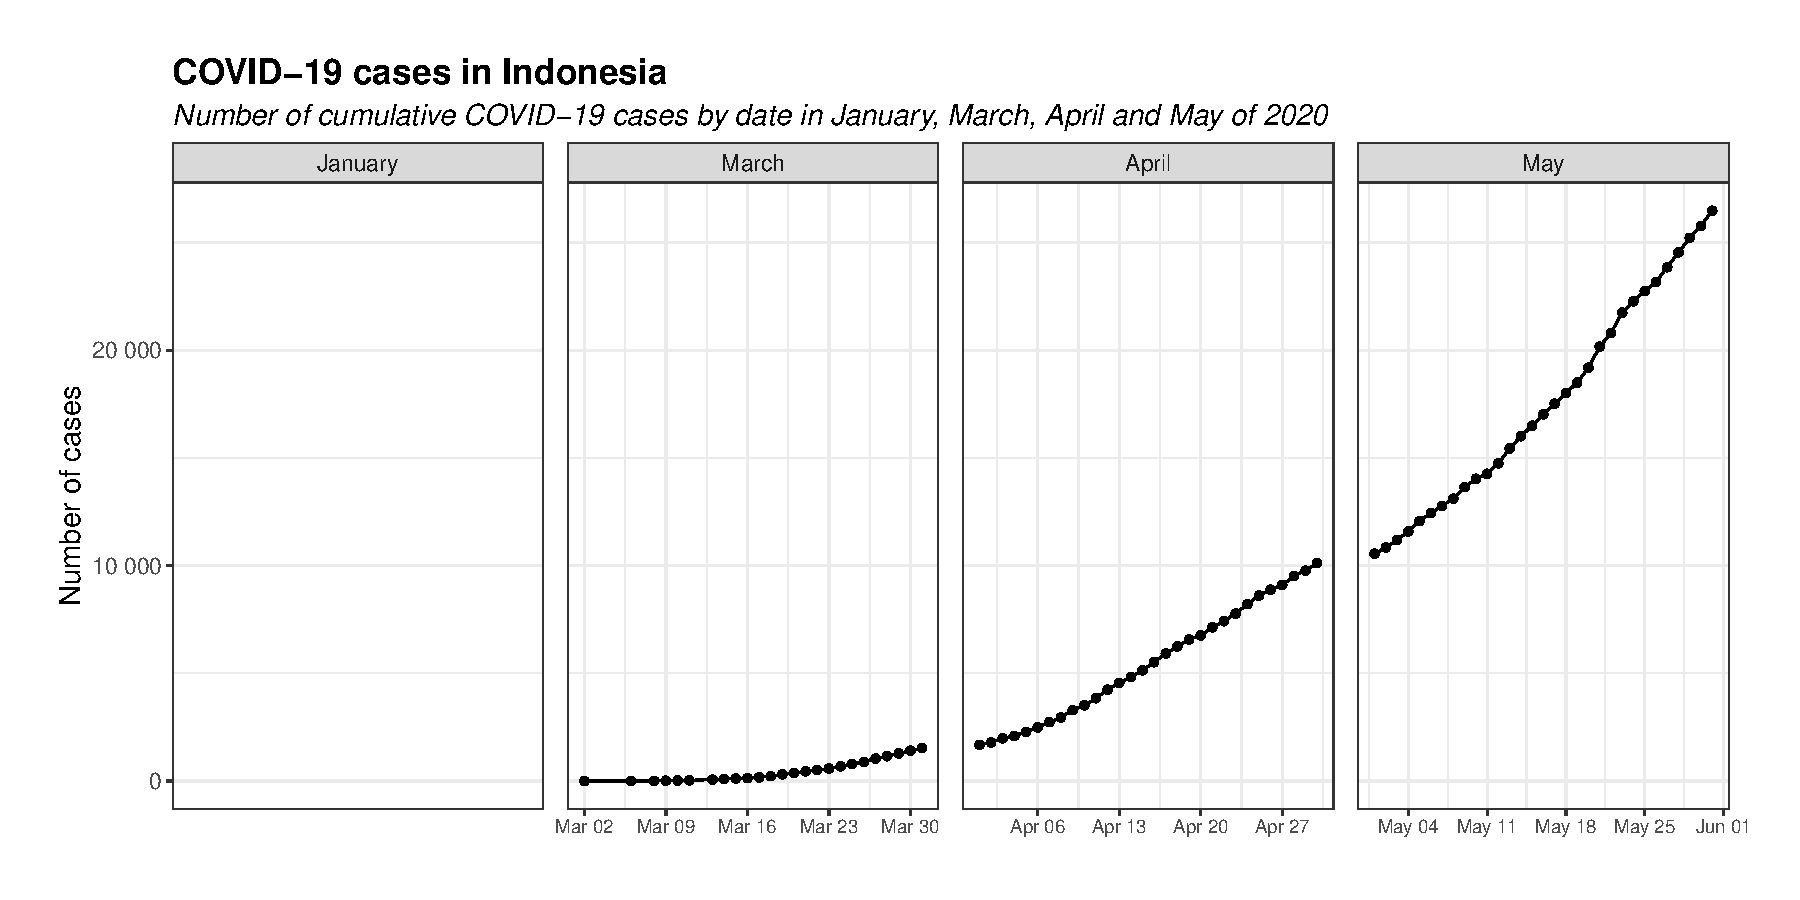
\includegraphics[scale=0.5]{v/IDN_2020_cumulative_cases.pdf}
        \end{center}
    \caption{\it Biểu đồ thể hiện thu thập dữ liệu nhiễm bệnh tích lũy cho từng tháng}
    \end{figure}
    \item Biểu đồ thể hiện thu thập dữ liệu tử vong tích lũy cho từng tháng\\
    Tương tự câu 1), sau đó ta tiến hành cộng tích luỹ số ca tử vong với nhau bằng $cumsum$
    \begin{lstlisting}[gobble=4]
    dataFile_deaths <- subset(dataFile_ISO, new_deaths>0 &
                    ((format(date,"%m")=="01") | (format(date,"%m")=="03") |
                    (format(date,"%m")=="04") | (format(date,"%m")=="05")) & 
                    format(date,"%Y")=="2020",
                    select = c(date, new_deaths))
    dataFile_deaths$new_deaths <- cumsum(dataFile_deaths$new_deaths)
    dataFile_deaths <- dataFile_deaths %>% mutate(month = as.numeric(format(dataFile_deaths$date,"%m"))) %>%
                                       mutate(month = month.name[month])
    dataFile_deaths$month = factor(dataFile_deaths$month, levels = c("January", "March", "April", "May"))
    dataFile_deaths_plot <- ggplot(data = dataFile_deaths, mapping = aes(x = date, y = new_deaths, label = new_deaths)) +
                        geom_line() + geom_point() + 
                        facet_grid(~ dataFile_deaths$month, scales = "free_x", drop = FALSE) +
                        labs(x = "",
                             y = "Number of deaths",
                             title = "COVID-19 deaths in Indonesia",
                             subtitle = "Number of cumulative COVID-19 deaths by date in January, March, April and May of 2020") +
                        theme_bw() + theme(text = element_text(size = 14)) +
                        theme(plot.title = element_text(face = "bold")) +
                        theme(plot.subtitle = element_text(face = "italic")) +
                        theme(axis.text.x = element_text(angle = 0, size = 9)) +
                        theme(plot.margin = margin(1,1.2,0.5,1, "cm")) +
                        theme(panel.spacing.x = unit(4, "mm")) +
                        scale_y_continuous(labels = label_number())
    ggsave(dataFile_deaths_plot, filename = paste(country_code,"2020_cumulative_deaths.pdf",sep="_"), width = 12, height = 6)
    \end{lstlisting}
    Kết quả
    
    \begin{figure}[H]
        \begin{center}
            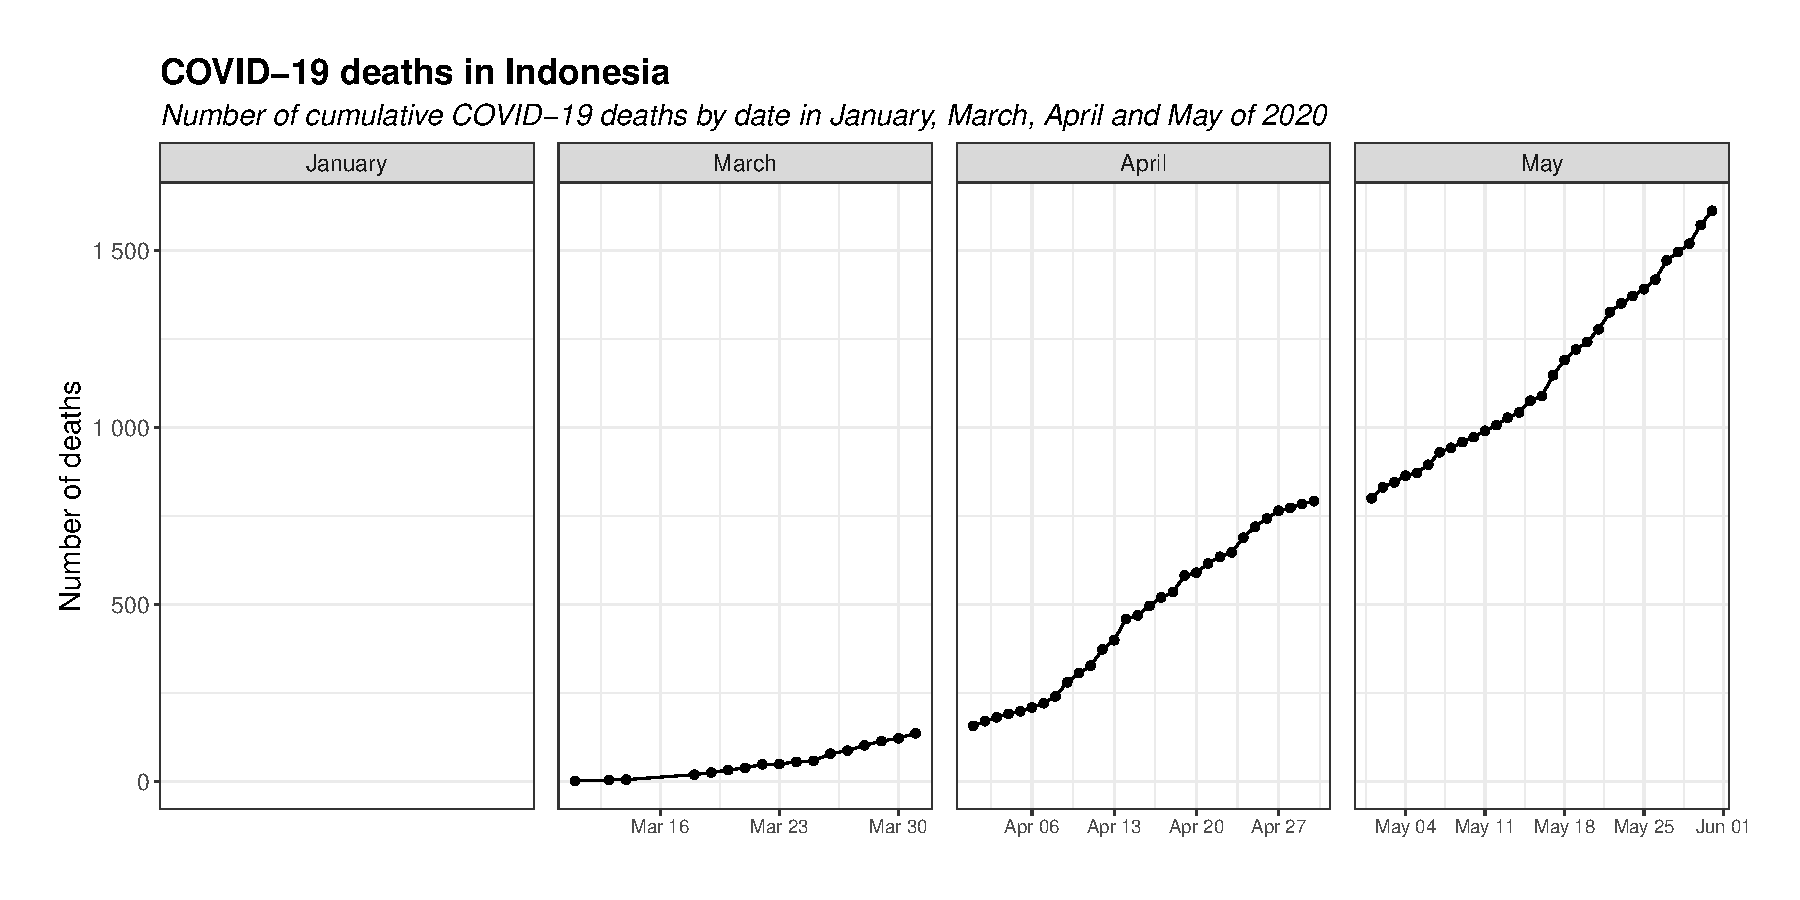
\includegraphics[scale=0.5]{v/IDN_2020_cumulative_deaths.pdf}
        \end{center}
    \caption{\it Biểu đồ thể hiện thu thập dữ liệu tử vong tích lũy cho từng tháng}
    \end{figure}
\end{enumerate}













\subsection{Nhiệm vụ vi}
\begin{enumerate}[vi)]
\item \textcolor{red}{Nhóm câu hỏi liên quan đến trực quan dữ liệu theo trung bình 7 ngày gần nhất}
\end{enumerate}
- Với mỗi quốc gia mà thuộc về nhóm, trên từng năm hãy vẽ biểu đồ thể hiện trục Ox là thời gian, trục Oy là nhiễm bệnh/tử vong. Hãy dùng 4 ký số của mã đề để vẽ 4 tháng tương ứng theo ký số đó. Nếu ký số là 0 thì lấy tháng là 10.

- Dùng trung bình của các ca nhiễm bệnh và tử vong được báo cáo trong 7 ngày gần nhất để loại trừ một số báo cáo không thường xuyên và đưa chúng ta đến gần hơn với con số hàng ngày.

\textbf{Xử lý chung}: Dùng trung bình của các ca nhiễm bệnh và tử vong được báo cáo trong 7 ngày gần nhất. Ta dùng vòng lặp $for$.
		
		\begin{lstlisting}
avg_nc_Jp_1_2020 <- c()
avg_nc_Jp_1_2020[1] <- Japan_nc_1_2020$new_cases[1]
avg_nc_Jp_1_2020[2] <- (Japan_nc_1_2020$new_cases[1] + Japan_nc_1_2020$new_cases[2])/2
avg_nc_Jp_1_2020[3] <- (Japan_nc_1_2020$new_cases[1] + Japan_nc_1_2020$new_cases[2] + Japan_nc_1_2020$new_cases[3])/3
avg_nc_Jp_1_2020[4] <- (Japan_nc_1_2020$new_cases[1] + Japan_nc_1_2020$new_cases[2] + Japan_nc_1_2020$new_cases[3] + Japan_nc_1_2020$new_cases[4])/4
avg_nc_Jp_1_2020[5] <- (Japan_nc_1_2020$new_cases[1] + Japan_nc_1_2020$new_cases[2] + Japan_nc_1_2020$new_cases[3] + Japan_nc_1_2020$new_cases[4] + Japan_nc_1_2020$new_cases[5])/5
avg_nc_Jp_1_2020[6] <- (Japan_nc_1_2020$new_cases[1] + Japan_nc_1_2020$new_cases[2] + Japan_nc_1_2020$new_cases[3] + Japan_nc_1_2020$new_cases[4] + Japan_nc_1_2020$new_cases[5] + Japan_nc_1_2020$new_cases[6])/6
for(i in 7:length(Japan_nc_1_2020$new_cases))
{
	avg_nc_Jp_1_2020[i]=
	(Japan_nc_1_2020$new_cases[i] + 
	Japan_nc_1_2020$new_cases[i-1] + 
	Japan_nc_1_2020$new_cases[i-2] + 
	Japan_nc_1_2020$new_cases[i-3] + 
	Japan_nc_1_2020$new_cases[i-4] + 
	Japan_nc_1_2020$new_cases[i-5] + Japan_nc_1_2020$new_cases[i-6])/7
}
	\end{lstlisting}
	
		Để tính số lượng tích lũy, ta cũng dùng vòng lặp for:
		
\begin{lstlisting}
acml_nc_Jp_1_2020 <- c()
acml_nc_Jp_1_2020[1] <- avg_nc_Jp_1_2020[1]
for(i in 2:length(avg_nc_Jp_1_2020))
{
	acml_nc_Jp_1_2020[i] <- avg_nc_Jp_1_2020[i] + acml_nc_Jp_1_2020[i-1]
}
	\end{lstlisting}
	
	Kết hợp 2 biến trung bình và tích lũy trên vào bảng trên:
		
\begin{lstlisting}
Japan_nc_1_2020 <- data.frame(Japan_nc_1_2020, avg_nc_Jp_1_2020, acml_nc_Jp_1_2020)
\end{lstlisting}
		
		Ta được:\\
		\begin{figure}[H]
	    \begin{center}
            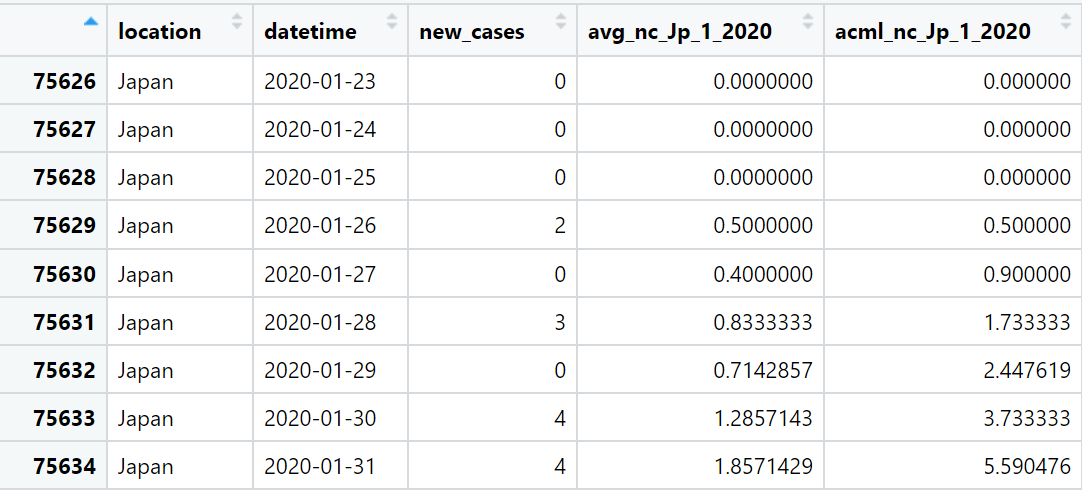
\includegraphics{vi/jp_nc_1_20201.png}
	    \end{center}
	   \vspace{+3mm}\caption{\it Bảng dữ liệu cho câu vi}
	   \end{figure}
	
Thực hiện tương tự các bước trên đối với những tháng khác và những quốc gia còn lại, cũng thực hiện tương tự khi lọc số liệu theo $new\_deaths$.\\
Từ các bảng số liệu đã lập, ta đã có đầy đủ dữ kiện để vẽ biểu đồ.\\
Khi vẽ biểu đồ, với các bảng số liệu rỗng, ta bỏ qua không xét.
\begin{enumerate}[1)]
    \item Biểu đồ thu thập nhiễm bệnh cho từng tháng
    
	Với trục Ox là trục thời gian, trục Oy là nhiễm bệnh, ta vẽ được biểu đồ đường, mỗi đường đại diện cho số ca nhiễm bệnh của 1 nước.\\
	\indent Với mỗi $geom\_line$ là một đường biểu thị cho số liệu $new\_cases$ của 1 bảng số liệu không rỗng\\[8pt]
	Ví dụ: Số ca nhiễm của tháng 1/2020\\
	\begin{lstlisting}
Newcases_1_2020 <- ggplot() + 
	geom_line(data=Japan_nc_1_2020, aes(x=datetime, y=avg_nc_Jp_1_2020, color = 'Japan')) +
	geom_line(data=Vietnam_nc_1_2020, aes(x=datetime, y=avg_nc_Vn_1_2020, color = 'Vietnam')) +
	labs(title = "Newcases 1-2020", x = "date", y = "new cases")
	\end{lstlisting}
	
	Kết quả
	\begin{figure}[H]
	    \begin{center}
	        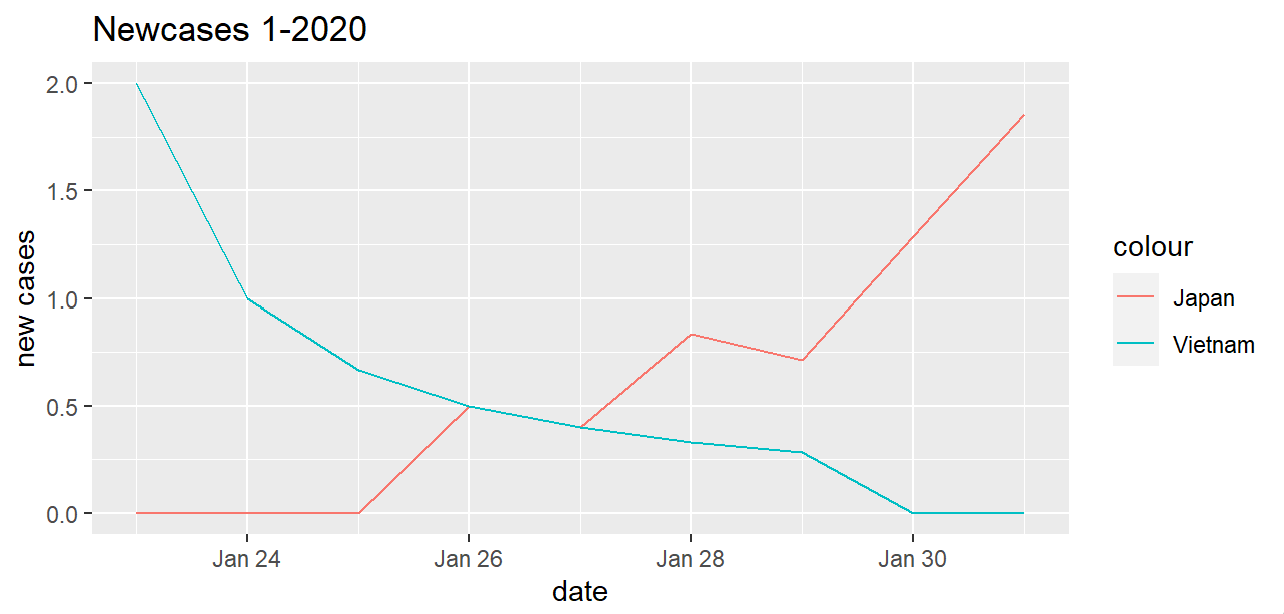
\includegraphics[scale=0.5]{vi/nc_1_2020}
	        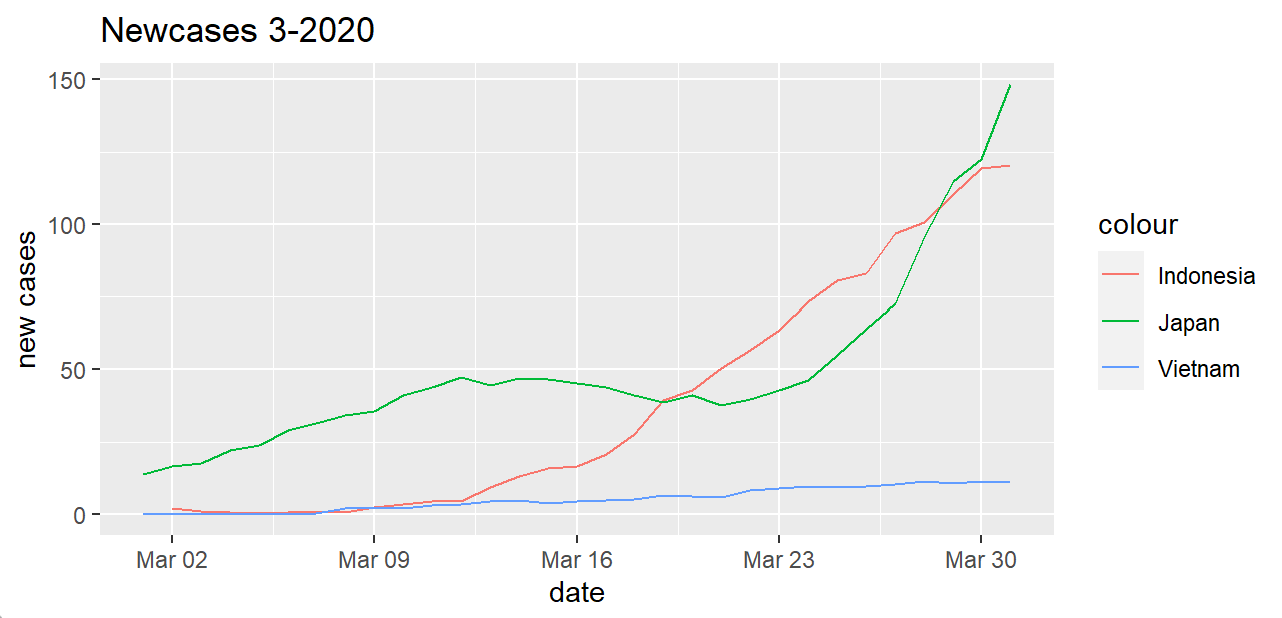
\includegraphics[scale=0.5]{vi/nc_3_2020}
    		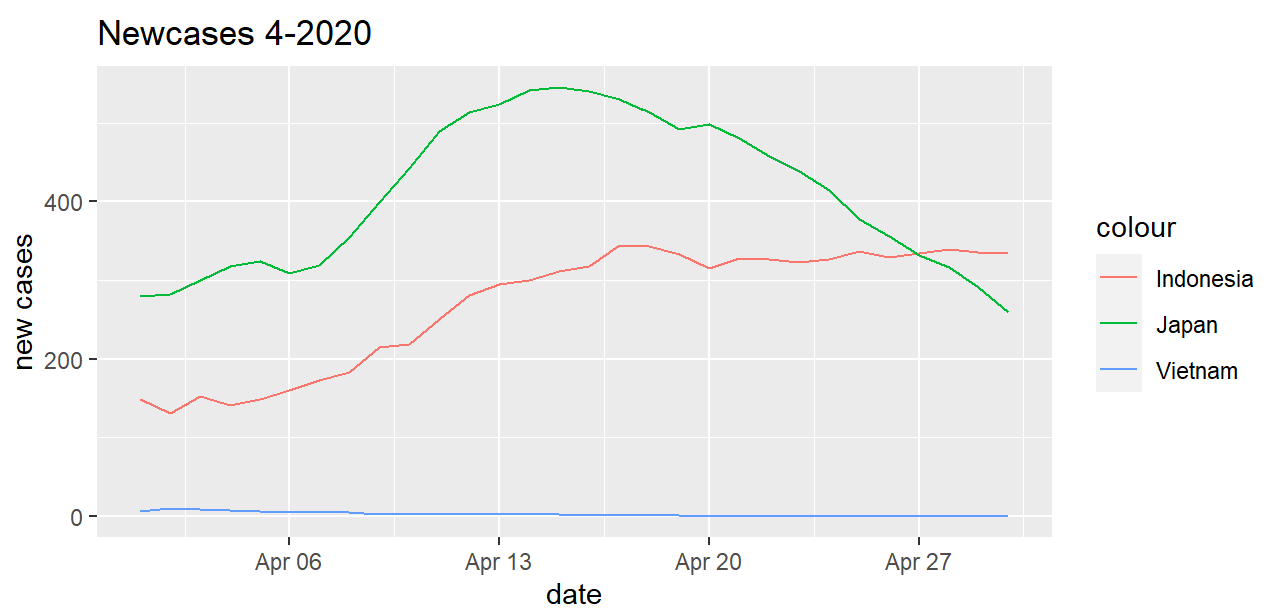
\includegraphics[scale=0.5]{vi/nc_4_2020}
    		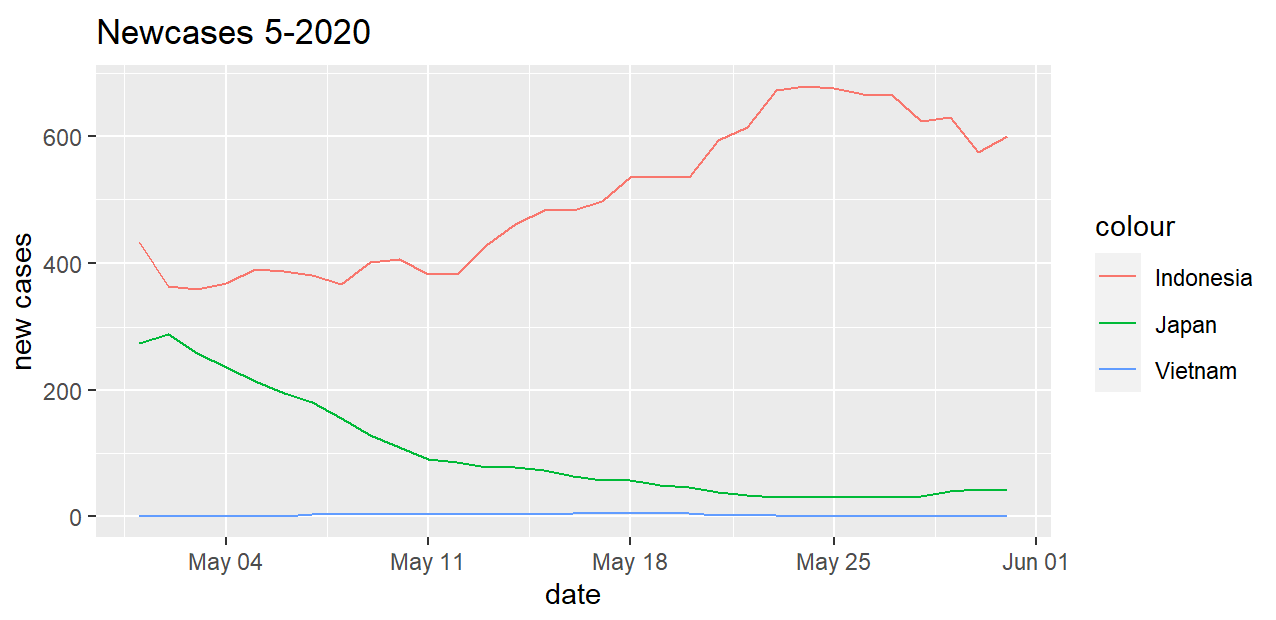
\includegraphics[scale=0.5]{vi/nc_5_2020}
    		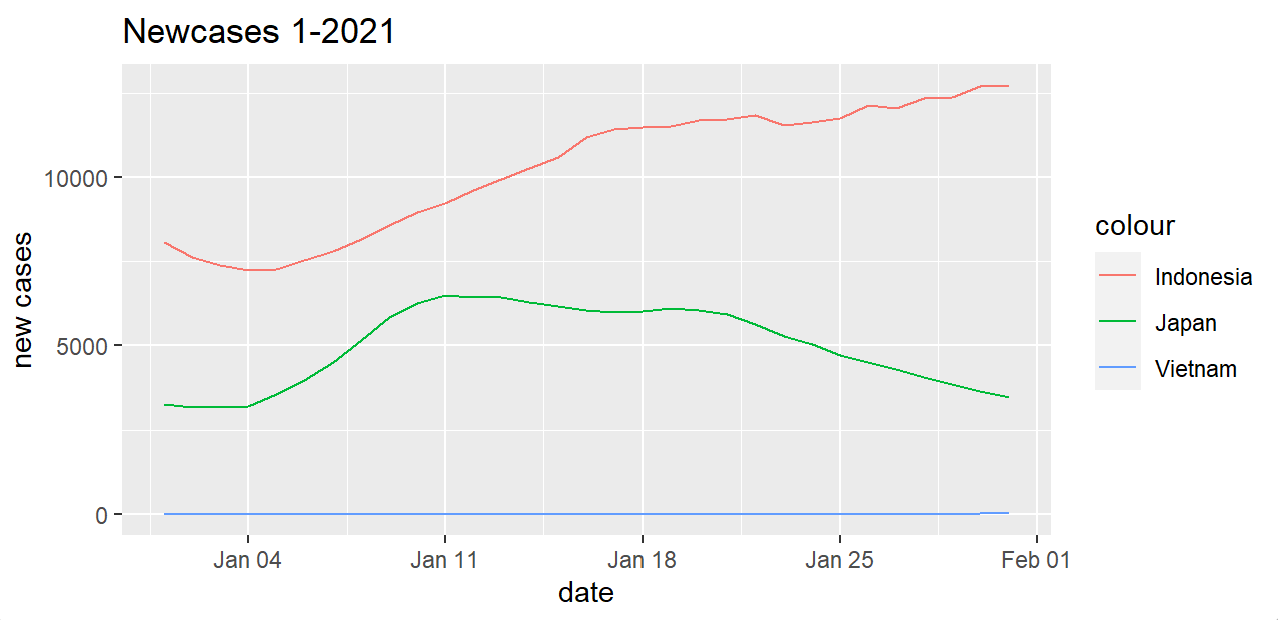
\includegraphics[scale=0.5]{vi/nc_1_2021}
	    \end{center}
	\end{figure}

	
	\begin{figure}[H]
	    \begin{center}
    		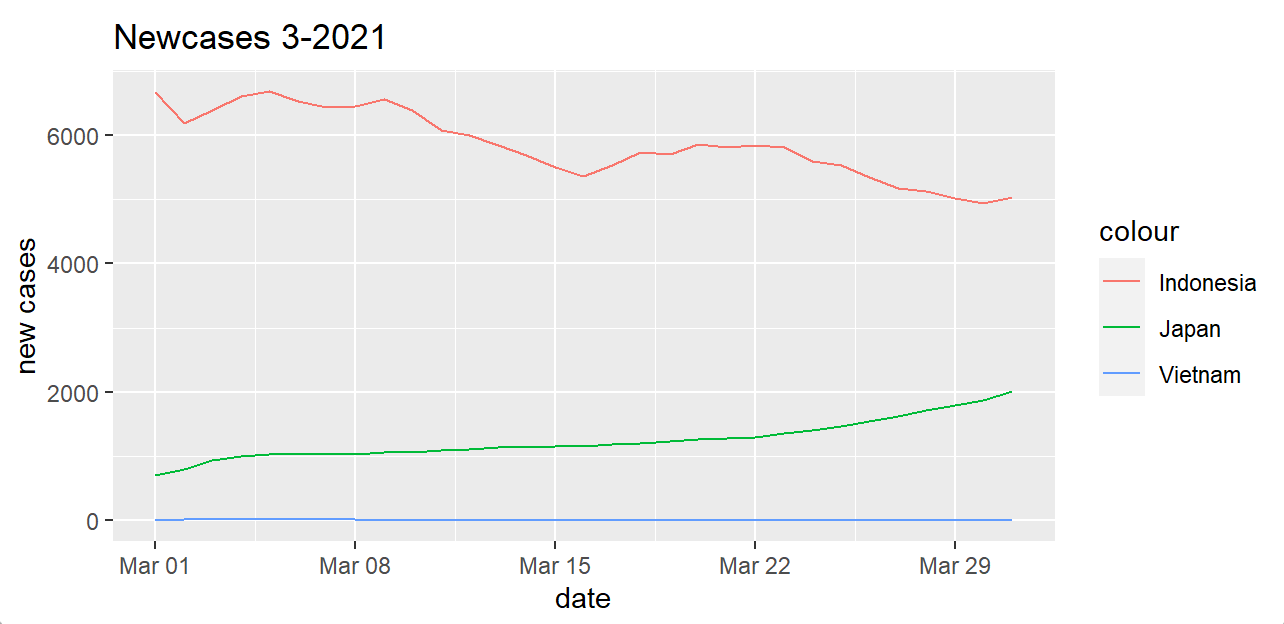
\includegraphics[scale=0.5]{vi/nc_3_2021}
    		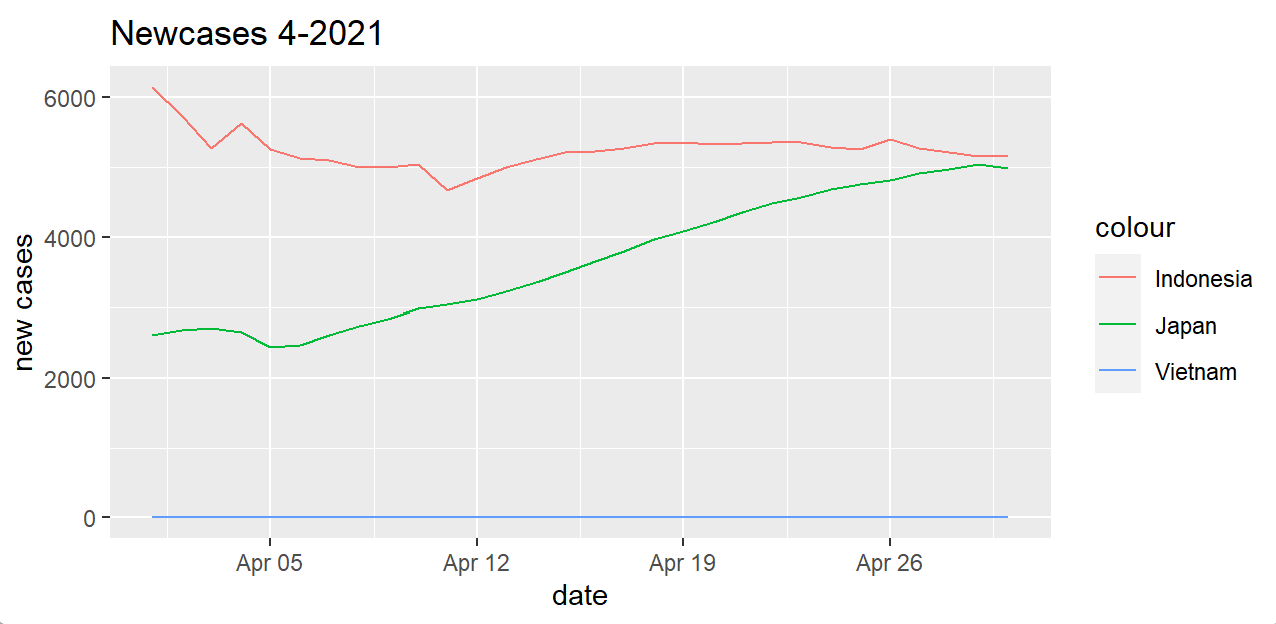
\includegraphics[scale=0.5]{vi/nc_4_2021}
    		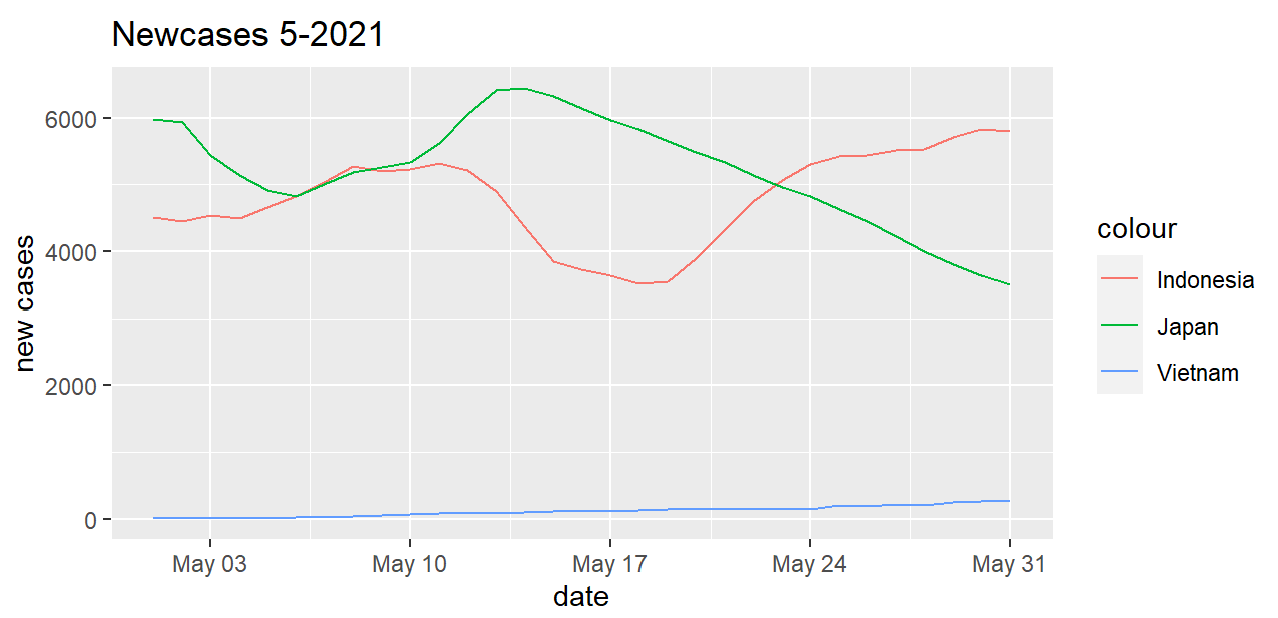
\includegraphics[scale=0.5]{vi/nc_5_2021}
    		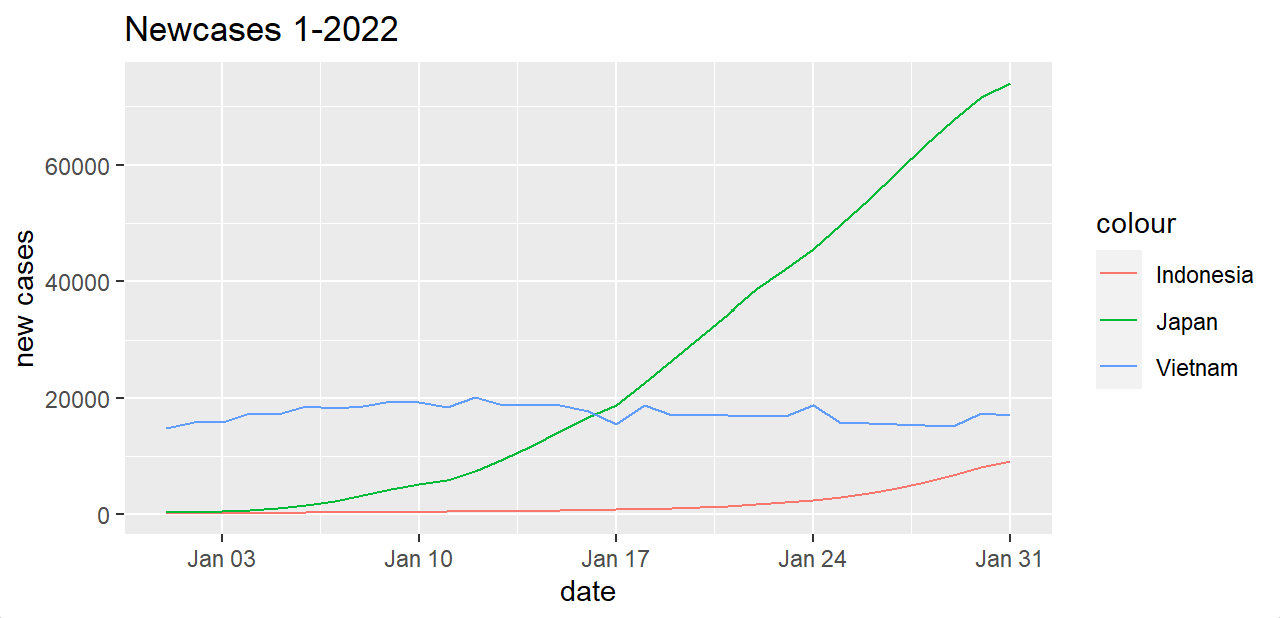
\includegraphics[scale=0.5]{vi/nc_1_2022}
	    \end{center}
	   \vspace{+3mm}\caption{\it Biểu đồ thu thập nhiễm bệnh theo từng tháng}
	   \end{figure}
	   
    \item Biểu đồ thu thập tử vong cho từng tháng
    
	Với trục Ox là trục thời gian, trục Oy là tử vong, ta vẽ được biểu đồ đường, mỗi đường đại diện cho số ca tử vong của 1 nước.\\
	\indent Với mỗi $geom\_line$ là một đường biểu thị cho $new\_deaths$ của 1 bảng số liệu không rỗng\\[8pt]
	Ví dụ: Ở tháng 1/2020 số liệu $new\_deaths$ của cả 3 nước Indonesia, Japan, Vietnam đều rỗng, ta bỏ qua.\\
	Ví dụ: Ở tháng 3/2020, hoàn toàn tương tự như câu 1, thay dữ liệu $new\_cases$ thành $new\_deaths$.

	
	Kết quả
	\begin{figure}[H]
	    \begin{center}
	        \includegraphics[scale=0.5]{vi/nd_3_2020}
	        \includegraphics[scale=0.5]{vi/nd_4_2020}
		    \includegraphics[scale=0.5]{vi/nd_5_2020}
		    \includegraphics[scale=0.5]{vi/nd_1_2021}
		    \includegraphics[scale=0.5]{vi/nd_3_2021}
	    \end{center}
	\end{figure}

	
	\begin{figure}[H]
	    \begin{center}
    		\includegraphics[scale=0.5]{vi/nd_4_2021}
    		\includegraphics[scale=0.5]{vi/nd_5_2021}
    		\includegraphics[scale=0.5]{vi/nd_1_2022}
	    \end{center}
	   \vspace{+3mm}\caption{\it Biểu đồ thu thập tử vong theo từng tháng}
	   \end{figure}
	   
    \item Biểu đồ thu thập gồm nhiễm bệnh và tử vong cho từng tháng
    
	Ở câu này, ta sẽ kết hợp biểu diễn số ca nhiễm và số ca tử vong trong cùng một biểu đồ bằng cách thêm các $geom\_line$ của $new\_cases$ và $new\_deaths$ (của các bảng dữ liệu khác rỗng) vào cùng một biểu đồ.\\[8pt] 
	Ví dụ: Đối với tháng 1/2020, các quốc gia đều không có ghi nhận ca tử vong nào, nên biểu đồ cần vẽ chính là biểu đồ thu thập ca nhiễm.\\
	Ví dụ: Đối với tháng 3/2020, ta có:
	
	\begin{lstlisting}
New_3_2020 <- ggplot() +
	geom_line(data=Indonesia_nc_3_2020, aes(x=datetime, y=avg_nc_Indo_3_2020, linetype = 'Newcases', color='Indonesia')) +
	geom_line(data=Japan_nc_3_2020, aes(x=datetime, y=avg_nc_Jp_3_2020, linetype = 'Newcases', color='Japan')) +
	geom_line(data=Vietnam_nc_3_2020, aes(x=datetime, y=avg_nc_Vn_3_2020, linetype = 'Newcases', color='Vietnam')) +
	geom_line(data=Indonesia_nd_3_2020, aes(x=datetime, y=avg_nd_Indo_3_2020, linetype = 'Newdeaths', color='Indonesia')) +
	geom_line(data=Japan_nd_3_2020, aes(x=datetime, y=avg_nd_Jp_3_2020, linetype = 'Newdeaths', color='Japan')) +
	labs(title = "Newcases and Newdeaths 3-2020", x = "date", y = "cases")
	\end{lstlisting}
	
	Kết quả
	\begin{figure}[H]
	    \begin{center}
            \includegraphics[scale=0.5]{vi/new_3_2020}
            \includegraphics[scale=0.5]{vi/new_4_2020}
			\includegraphics[scale=0.5]{vi/new_5_2020}
			\includegraphics[scale=0.5]{vi/new_1_2021}
			\includegraphics[scale=0.5]{vi/new_3_2021}
	    \end{center}
	\end{figure}

	
	\begin{figure}[H]
	    \begin{center}
			\includegraphics[scale=0.5]{vi/new_4_2021}
			\includegraphics[scale=0.5]{vi/new_5_2021}
			\includegraphics[scale=0.5]{vi/new_1_2022}
	    \end{center}
	   \vspace{+3mm}\caption{\it Biểu đồ thu thập nhiễm bệnh và tử vong cho từng tháng}
	   \end{figure}	
	   
    \item Biểu đồ thu thập nhiễm bệnh gồm 2 tháng cuối của năm
    
	Đối với 2 tháng cuối năm, đầu tiên ta cũng lọc dữ liệu như các tháng khác đã làm.\\[8pt]
	Ví dụ: Đối với 2 tháng cuối năm 2020 của Indonesia\\
	Ta có:
	\begin{lstlisting}
Indonesia_nc_11_12_2020 <- na.omit(Indonesia_nc[Indonesia_nc$datetime >= "2020-11-01" & Indonesia_nc$datetime <= "2020-12-31",])
avg_nc_Indo_11_12_2020 <- c()
avg_nc_Indo_11_12_2020[1] <- Indonesia_nc_11_12_2020$new_cases[1]
avg_nc_Indo_11_12_2020[2] <- (Indonesia_nc_11_12_2020$new_cases[1] + Indonesia_nc_11_12_2020$new_cases[2])/2
avg_nc_Indo_11_12_2020[3] <- (Indonesia_nc_11_12_2020$new_cases[1] + Indonesia_nc_11_12_2020$new_cases[2] + Indonesia_nc_11_12_2020$new_cases[3])/3
avg_nc_Indo_11_12_2020[4] <- (Indonesia_nc_11_12_2020$new_cases[1] + Indonesia_nc_11_12_2020$new_cases[2] + Indonesia_nc_11_12_2020$new_cases[3] + Indonesia_nc_11_12_2020$new_cases[4])/4
avg_nc_Indo_11_12_2020[5] <- (Indonesia_nc_11_12_2020$new_cases[1] + Indonesia_nc_11_12_2020$new_cases[2] + Indonesia_nc_11_12_2020$new_cases[3] + Indonesia_nc_11_12_2020$new_cases[4] + Indonesia_nc_11_12_2020$new_cases[5])/5
avg_nc_Indo_11_12_2020[6] <- (Indonesia_nc_11_12_2020$new_cases[1] + Indonesia_nc_11_12_2020$new_cases[2] + Indonesia_nc_11_12_2020$new_cases[3] + Indonesia_nc_11_12_2020$new_cases[4] + Indonesia_nc_11_12_2020$new_cases[5] + Indonesia_nc_11_12_2020$new_cases[6])/6
for(i in 7:length(Indonesia_nc_11_12_2020$new_cases))
{
    avg_nc_Indo_11_12_2020[i]=(Indonesia_nc_11_12_2020$new_cases[i] + Indonesia_nc_11_12_2020$new_cases[i-1] + Indonesia_nc_11_12_2020$new_cases[i-2] + Indonesia_nc_11_12_2020$new_cases[i-3] + Indonesia_nc_11_12_2020$new_cases[i-4] + Indonesia_nc_11_12_2020$new_cases[i-5] + Indonesia_nc_11_12_2020$new_cases[i-6])/7
}
acml_nc_Indo_11_12_2020 <- c()
acml_nc_Indo_11_12_2020[1] <- avg_nc_Indo_11_12_2020[1]
for(i in 2:length(avg_nc_Indo_11_12_2020))
{
	acml_nc_Indo_11_12_2020[i] <- avg_nc_Indo_11_12_2020[i] + acml_nc_Indo_11_12_2020[i-1]
}
Indonesia_nc_11_12_2020 <- data.frame(Indonesia_nc_11_12_2020, avg_nc_Indo_11_12_2020, acml_nc_Indo_11_12_2020)
	\end{lstlisting}
	
	Bảng dữ liệu thu được:\\[8pt]
	\begin{figure}[H]
	    \begin{center}
            \includegraphics[scale=0.6]{vi/bang_indo_11_12_2020}
	    \end{center}
	    \vspace{+3mm}\caption{\it Bảng dữ liệu cho câu vi.4}
	\end{figure}
	
	
	Thực hiện tương tự cho Japan và Vietnam ta cũng được 2 bảng dữ liệu nữa.\\[8pt]
	Sau đó ta tiến hành vẽ biểu đồ dựa trên các bảng dữ liệu vừa tìm được\\
	
	\begin{lstlisting}
Newcases_11_12_2020 <- ggplot() +
	geom_line(data=Indonesia_nc_11_12_2020, aes(x=datetime, y=avg_nc_Indo_11_12_2020, color = 'Indonesia')) +
	geom_line(data=Japan_nc_11_12_2020, aes(x=datetime, y=avg_nc_Jp_11_12_2020, color = 'Japan')) +
	geom_line(data=Vietnam_nc_11_12_2020, aes(x=datetime, y=avg_nc_Vn_11_12_2020, color = 'Vietnam')) +
	labs(title = "Newcases in the last 2 months of 2020", x = "date", y = "new cases")
	\end{lstlisting}

	Kết quả
	\begin{figure}[H]
	    \begin{center}
            \includegraphics[scale=0.5]{vi/nc_11_12_2020}
            \includegraphics[scale=0.5]{vi/nc_11_12_2021}
	    \end{center}
	    \vspace{+3mm}\caption{\it Biểu đồ thu thập nhiễm bệnh cho 2 tháng cuối năm}
	\end{figure}
	
    \item Biểu đồ thu thập tử vong gồm 2 tháng cuối của năm
    
	Câu hỏi này hoàn toàn tương tự như câu 4, chỉ thay dữ liệu $new\_cases$ thành $new\_deaths$

	Kết quả
	\begin{figure}[H]
	    \begin{center}
            \includegraphics[scale=0.5]{vi/nd_11_12_2020}
            \includegraphics[scale=0.5]{vi/nd_11_12_2021}
	    \end{center}
	    \vspace{+3mm}\caption{\it Biểu đồ thu thập tử vong cho 2 tháng cuối năm}
	\end{figure}
	
    \item Biểu đồ thu thập gồm nhiễm bệnh và tử vong gồm 2 tháng cuối của năm
    
	Kết hợp các đường biểu diễn ca nhiễm và các đường biểu diễn tử vong trong cùng một biểu đồ như sau:
	\begin{lstlisting}
New_11_12_2020 <- ggplot() +
	geom_line(data=Indonesia_nc_11_12_2020, aes(x=datetime, y=avg_nc_Indo_11_12_2020, linetype = 'Newcases', color='Indonesia')) +
	geom_line(data=Japan_nc_11_12_2020, aes(x=datetime, y=avg_nc_Jp_11_12_2020, linetype = 'Newcases', color='Japan')) +
	geom_line(data=Vietnam_nc_11_12_2020, aes(x=datetime, y=avg_nc_Vn_11_12_2020, linetype = 'Newcases', color='Vietnam')) +
	geom_line(data=Indonesia_nd_11_12_2020, aes(x=datetime, y=avg_nd_Indo_11_12_2020, linetype = 'Newdeaths', color='Indonesia')) +
	geom_line(data=Japan_nd_11_12_2020, aes(x=datetime, y=avg_nd_Jp_11_12_2020, linetype = 'Newdeaths', color='Japan')) +
	geom_line(data=Vietnam_nd_11_12_2020, aes(x=datetime, y=avg_nd_Vn_11_12_2020, linetype = 'Newdeaths', color='Vietnam')) +
	labs(title = "Newcases and Newdeaths in the last 2 months of 2020", x = "date", y = "cases")
	\end{lstlisting}
	
	Kết quả
	\begin{figure}[H]
	    \begin{center}
            \includegraphics[scale=0.5]{vi/new_11_12_2020}
            \includegraphics[scale=0.5]{vi/new_11_12_2021}
	    \end{center}
	    \vspace{+3mm}\caption{\it Biểu đồ thu thập nhiễm bệnh và tử vong cho 2 tháng cuối năm}
	\end{figure}
	
    \item Biểu đồ thu thập nhiễm bệnh tích lũy cho từng tháng
    
	Với đề yêu cầu là biểu đồ thu thập tích lũy, chỉ khác một tí là ta sẽ vẽ dựa trên biến tích lũy đã tạo thay vì các biến giá trị trung bình như các câu trên.\\[8pt]
	Ví dụ với tháng 1/2020:
	\begin{lstlisting}
Acml_Newcases_1_2020 <- ggplot() + 
	geom_line(data=Japan_nc_1_2020, aes(x=datetime, y=acml_nc_Jp_1_2020, color = 'Japan')) +
	geom_line(data=Vietnam_nc_1_2020, aes(x=datetime, y=acml_nc_Vn_1_2020, color = 'Vietnam')) +
	labs(title = "Cumulative Newcases 1-2020", x = "date", y = "number of accumulation")
	\end{lstlisting}
	
	Kết quả
	\begin{figure}[H]
	    \begin{center}
            \includegraphics[scale=0.5]{vi/cml_nc_1_2020}
    		\includegraphics[scale=0.5]{vi/cml_nc_3_2020}
    		\includegraphics[scale=0.5]{vi/cml_nc_4_2020}
    		\includegraphics[scale=0.5]{vi/cml_nc_5_2020}
    		\includegraphics[scale=0.5]{vi/cml_nc_1_2021}
	    \end{center}
	\end{figure}
	
	\begin{figure}[H]
	    \begin{center}
    		\includegraphics[scale=0.5]{vi/cml_nc_3_2021}
    		\includegraphics[scale=0.5]{vi/cml_nc_4_2021}
    		\includegraphics[scale=0.5]{vi/cml_nc_5_2021}
    		\includegraphics[scale=0.5]{vi/cml_nc_1_2022}
	    \end{center}
	    \vspace{+3mm}\caption{\it Biểu đồ thu thập nhiễm bệnh tích lũy cho từng tháng}
	\end{figure}
	
    \item Biểu đồ thu thập tử vong tích lũy cho từng tháng
    
    Thực hiện hoàn toàn tương tự như câu 7, thay dữ liệu $new\_cases$ thành $new\_deaths$.
	
	Kết quả
	\begin{figure}[H]
	    \begin{center}
            \includegraphics[scale=0.5]{vi/cml_nd_3_2020}
    		\includegraphics[scale=0.5]{vi/cml_nd_4_2020}
    		\includegraphics[scale=0.5]{vi/cml_nd_5_2020}
    		\includegraphics[scale=0.5]{vi/cml_nd_1_2021}
	    \end{center}
	\end{figure}
	
	\begin{figure}[H]
	    \begin{center}
    		\includegraphics[scale=0.5]{vi/cml_nd_3_2021}
    		\includegraphics[scale=0.5]{vi/cml_nd_4_2021}
    		\includegraphics[scale=0.5]{vi/cml_nd_5_2021}
    		\includegraphics[scale=0.5]{vi/cml_nd_1_2022}
	    \end{center}
	    \vspace{+3mm}\caption{\it Biểu đồ thu thập tử vong tích lũy cho từng tháng}
	\end{figure}
	
\end{enumerate}


	










\subsection{Nhiệm vụ vii}
\begin{enumerate}[vii)]
\item \textcolor{red}{Nhóm câu hỏi liên quan đến tất cả quốc gia theo thời gian là tháng}
\end{enumerate}

- Trên từng năm hãy vẽ biểu đồ thể hiện trục Ox là thời gian, trục Oy là nhiễm bệnh/tử vong. Hãy dùng 4 ký số của mã đề để vẽ 4 tháng tương ứng theo ký số đó. Nếu ký số là 0 thì lấy tháng là 10. 

Đây là nhóm câu hỏi liên quan đến tháng, nên bước đầu tiên ta đưa format chuẩn về ngày tháng năm để tiện xử lý.
\begin{lstlisting}
dataFile$date <- strptime(dataFile$date, format="%m/%d/%Y")
\end{lstlisting}
\begin{enumerate}[1)]
\item Vẽ biểu đồ thể hiện thu thập dữ liệu nhiễm bệnh theo thời gian là tháng của tất cả quốc gia.\\
Với câu hỏi này, ta sử dụng hàm $sum()$ với điều kiện để tính theo yêu cầu.
\begin{lstlisting}
  data_newcases <- c(rep(0,times=12))
  data_newcases[1] <- sum(dataFile[which(dataFile$new_cases>0
                                    &dataFile$iso_code!="OWID_WRL"
                                    &format(dataFile$date,"%Y")=="2020"
                                    &format(dataFile$date,"%m")=="01"),5])
  data_newcases[2] <- sum(dataFile[which(dataFile$new_cases>0
                                    &dataFile$iso_code!="OWID_WRL"
                                    &format(dataFile$date,"%Y")=="2020"
                                    &format(dataFile$date,"%m")=="03"),5])
  data_newcases[3] <- sum(dataFile[which(dataFile$new_cases>0
                                    &dataFile$iso_code!="OWID_WRL"
                                    &format(dataFile$date,"%Y")=="2020"
                                    &format(dataFile$date,"%m")=="04"),5])
  data_newcases[4] <- sum(dataFile[which(dataFile$new_cases>0
                                    &dataFile$iso_code!="OWID_WRL"
                                    &format(dataFile$date,"%Y")=="2020"
                                    &format(dataFile$date,"%m")=="05"),5])
\end{lstlisting}
Những tháng sau hiện thực code hoàn toàn tương tự như trên.

Khi đã tổng hợp dữ liệu, ta vẽ biểu đồ cột với hàm $barplot()$ và xuất hình ảnh bằng hàm $png()$, cuối cùng kết thúc bằng hàm $dev.off()$ để đóng file png.
\begin{lstlisting}
png(file = "newcase.png",width=1000)
barplot(data_newcases,
          main="NEW CASES ALL OVER THE WORLD",
          # beside=TRUE,
          col="tomato",
          names.arg=c("01/2020","03/2020","04/2020","05/2020",
                        "01/2021","03/2021","04/2021","05/2021",
                        "01/2022","03/2022","04/2022","05/2022"),
          ylab="Cases",
          xlab="Year",
        )
dev.off()
\end{lstlisting}
Kết quả
\begin{figure}[H]
        \begin{center}
            \includegraphics[scale=0.4]{vii/vii1.png} 
        \end{center}
        \vspace{+3mm}\caption{\it Biểu đồ nhiễm bệnh theo từng tháng của tất cả quốc gia}
    \end{figure}
\item Biểu đồ thể hiện thu thập dữ liệu tử vong theo thời gian là tháng của tất cả quốc gia

Tương tự với ý 1, ta chỉ cần thay vì thu thập dữ liệu $new\_cases$, ta sẽ lấy dữ liệu là $new\_deaths$.
\begin{lstlisting}
vii2<-function()
{
  data_newdeath <- c(rep(0,times=12))
  data_newdeath[1] <- sum(dataFile[which(dataFile$new_deaths>0&
                                    dataFile$iso_code!="OWID_WRL"&
                                    format(dataFile$date,"%Y")=="2020"&
                                    format(dataFile$date,"%m")=="01"),5])
  data_newdeath[2] <- sum(dataFile[which(dataFile$new_deaths>0&
                                    dataFile$iso_code!="OWID_WRL"&
                                    format(dataFile$date,"%Y")=="2020"&
                                    format(dataFile$date,"%m")=="03"),5])
  data_newdeath[3] <- sum(dataFile[which(dataFile$new_deaths>0&
                                    dataFile$iso_code!="OWID_WRL"&
                                    format(dataFile$date,"%Y")=="2020"&
                                    format(dataFile$date,"%m")=="04"),5])
  data_newdeath[4] <- sum(dataFile[which(dataFile$new_deaths>0&
                                    dataFile$iso_code!="OWID_WRL"&
                                    format(dataFile$date,"%Y")=="2020"&
                                    format(dataFile$date,"%m")=="05"),5])
  
  png(file = "vii2.png",width=1000)
  barplot(data_newdeath,
          main="NEW DEATHS CASES ALL OVER THE WORLD",
          # beside=TRUE,
          col="tomato",
          names.arg=c("01/2020","03/2020","04/2020","05/2020",
                    "01/2021","03/2021","04/2021","05/2021",
                    "01/2022","03/2022","04/2022","05/2022"),
          ylab="Case",
          xlab="Year",
  )
  dev.off()
}
\end{lstlisting}
Kết quả
\begin{figure}[H]
        \begin{center}
            \includegraphics[scale=0.35]{vii/vii2.png} 
        \end{center}
        \vspace{+3mm}\caption{\it Biểu đồ tử vong theo từng tháng của tất cả quốc gia}
    \end{figure}
\item Biểu đồ thể hiện thu thập dữ liệu nhiễm bệnh theo thời gian là 2 tháng cuối của năm của tất cả quốc gia.

Với câu này, trong hàm $sum()$, ta lấy điều kiện là tháng 11 và 12 của từng năm. Sau đó lưu vào một ma trận để vẽ biểu đồ.
\begin{lstlisting}
  data_newcases_2months_2020 <- sum(dataFile[which(dataFile$new_cases>0&
                                        dataFile$iso_code!="OWID_WRL"&
                                        format(dataFile$date,"%Y")=="2020"&
                                        (format(dataFile$date,"%m")=="12"|
                                        format(dataFile$date,"%m")=="11")),5]) 
  data_newcases_2months_2021 <- sum(dataFile[which(dataFile$new_cases>0&
                                        dataFile$iso_code!="OWID_WRL"&
                                        format(dataFile$date,"%Y")=="2021"&
                                        (format(dataFile$date,"%m")=="12"|
                                        format(dataFile$date,"%m")=="11")),5])
  data_newcases_2months_2022 <- sum(dataFile[which(dataFile$new_cases>0&
                                        dataFile$iso_code!="OWID_WRL"&
                                        format(dataFile$date,"%Y")=="2022"&
                                        (format(dataFile$date,"%m")=="12"|
                                        format(dataFile$date,"%m")=="11")),5])
  data_newcases_2months <- c(data_newcases_2months_2020,data_newcases_2months_2021,data_newcases_2months_2022)
\end{lstlisting}
Ta tiếp tục vẽ biểu đồ bằng hàm barplot và xuất ra file png.
\begin{lstlisting}
png(file="vii3.png")
barplot(data_newcases_2months,
          main="NEW CASES ALL OVER THE WORLD IN LAST 2 MONTHS",
          col="tomato",
          ylab="Cases",
          xlab="Year",
          names.arg=c("2020","2021","2022"),
        )
dev.off()
\end{lstlisting}
Kết quả:
\begin{figure}[H]
        \begin{center}
            \includegraphics[scale=0.45]{vii/vii3.png} 
        \end{center}
        \vspace{+3mm}\caption{\it Biểu đồ nhiễm bệnh 2 tháng cuối của mỗi năm.}
    \end{figure}
\item Biểu đồ thể hiện thu thập dữ liệu tử vong theo thời gian là 2 tháng cuối của năm của tất cả quốc gia.

Tương tự với ý 3, ta thay dữ liệu $new\_cases$ thành $new\_deaths$.
\begin{lstlisting}
data_deathcases_2months_2020 <- sum(dataFile[which(dataFile$new_deaths>0&
                                    dataFile$iso_code!="OWID_WRL"&
                                    format(dataFile$date,"%Y")=="2020"&
                                    (format(dataFile$date,"%m")=="12"|
                                    format(dataFile$date,"%m")=="11")),6]) 
  data_deathcases_2months_2021 <- sum(dataFile[which(dataFile$new_deaths>0&
                                    dataFile$iso_code!="OWID_WRL"&
                                    format(dataFile$date,"%Y")=="2021"&
                                    (format(dataFile$date,"%m")=="12"|
                                    format(dataFile$date,"%m")=="11")),6])
  data_deathcases_2months_2022 <- sum(dataFile[which(dataFile$new_deaths>0&
                                     dataFile$iso_code!="OWID_WRL"&
                                     format(dataFile$date,"%Y")=="2022"&
                                     (format(dataFile$date,"%m")=="12"|
                                     format(dataFile$date,"%m")=="11")),6])
  data_deathcases_2months <- c(data_deathcases_2months_2020,data_deathcases_2months_2021,data_deathcases_2months_2022)
  png(file="vii4.png")
  barplot(data_deathcases_2months,
          main="NEW DEATH CASES ALL OVER THE WORLD IN LAST 2 MONTHS",
          col="tomato",
          ylab="Cases",
          xlab="Year",
          names.arg=c("2020","2021","2022"),
  )
  dev.off()
\end{lstlisting}
Kết quả:
\begin{figure}[H]
        \begin{center}
            \includegraphics[scale=0.45]{vii/vii4.png} 
        \end{center}
        \vspace{+3mm}\caption{\it Biểu đồ tử vong 2 tháng cuối của mỗi năm.}
    \end{figure}
\item Biểu đồ thể hiện thu thập dữ liệu nhiễm bệnh tương đối tích lũ y2 tháng cuối của năm của tất cả quốc gia.\\
Với bài toán tương đối tích lũy, ta sẽ tính dữ liệu cộng dồn.
\begin{lstlisting}
  data_newcases_20 <- c(0,0)
  data_newcases_20[1] <- sum(dataFile[which(dataFile$new_cases>0&
                                    dataFile$iso_code!="OWID_WRL"&
                                    format(dataFile$date,"%Y")=="2020"&
                                    format(dataFile$date,"%m")=="11"),5]) 
  data_newcases_20[2] <- sum(dataFile[which(dataFile$new_cases>0&
                                    dataFile$iso_code!="OWID_WRL"&
                                    format(dataFile$date,"%Y")=="2020"&
                                    (format(dataFile$date,"%m")=="12"|
                                    format(dataFile$date,"%m")=="11")),5]) 
  data_newcases_21 <- c(0,0)
  data_newcases_21[1] <- sum(dataFile[which(dataFile$new_cases>0&
                                    dataFile$iso_code!="OWID_WRL"&
                                    format(dataFile$date,"%Y")=="2021"&
                                    format(dataFile$date,"%m")=="11"),5]) 
  data_newcases_21[2] <- sum(dataFile[which(dataFile$new_cases>0&
                                    dataFile$iso_code!="OWID_WRL"&
                                    format(dataFile$date,"%Y")=="2021"&
                                    (format(dataFile$date,"%m")=="12"|
                                    format(dataFile$date,"%m")=="11")),5]) 
  data_newcases_22 <- c(0,0)
  data_newcases_22[1] <- sum(dataFile[which(dataFile$new_cases>0&
                                    dataFile$iso_code!="OWID_WRL"&
                                    format(dataFile$date,"%Y")=="2022"&
                                    format(dataFile$date,"%m")=="11"),5]) 
  data_newcases_22[2] <- sum(dataFile[which(dataFile$new_cases>0&
                                     dataFile$iso_code!="OWID_WRL"&
                                     format(dataFile$date,"%Y")=="2022"&
                                     (format(dataFile$date,"%m")=="12"|
                                     format(dataFile$date,"%m")=="11")),5]) 
\end{lstlisting}
Vì đây là nhiều vector nên ta tạo một dataframe lưu dữ liệu để vẽ biểu đồ
\begin{lstlisting}
data_newcase_multi <- data.frame(data_newcases_20,data_newcases_21,data_newcases_22)
\end{lstlisting}
Cuối cùng là dùng hàm barplot để vẽ biểu đồ.
\begin{lstlisting}
  png(file="vii5.png")
  barplot(as.matrix(data_newcase_multi),
          main="DATA NEW CASE MULTI",
          ylab="Cases", xlab="Year", beside=TRUE,
          col=c("tomato","steelblue2"), legend.text=c("November","December"),
          args.legend=list(x="topright"), names.arg=c("2020","2021","2022"),)
  dev.off()
\end{lstlisting}
Kết quả
\begin{figure}[H]
        \begin{center}
            \includegraphics[scale=0.3]{vii/vii5.png} 
        \end{center}
        \vspace{+3mm}\caption{\it Biểu đồ thể hiện nhiễm bệnh tương đối tích lũy 2 tháng cuối năm tất cả quốc gia.}
    \end{figure}
\item Biểu đồ thể hiện thu thập dữ liệu tử vong tương đối tích lũy theo thời gian là 2 tháng cuối của năm của tất cả quốc gia\\
Tương tự với ý 5, ta thay dữ liệu từ $new\_cases$ thành $new\_deaths$.
\begin{lstlisting}
data_deathscases_20 <- c(0,0)
  data_deathscases_20[1] <- sum(dataFile[which(dataFile$new_deaths>0&
                                    dataFile$iso_code!="OWID_WRL"&
                                    format(dataFile$date,"%Y")=="2020"&
                                    format(dataFile$date,"%m")=="11"),6]) 
  data_deathscases_20[2] <- sum(dataFile[which(dataFile$new_deaths>0&
                                    dataFile$iso_code!="OWID_WRL"&
                                    format(dataFile$date,"%Y")=="2020"&
                                    (format(dataFile$date,"%m")=="12"|
                                    format(dataFile$date,"%m")=="11")),6]) 
  data_deathscases_21 <- c(0,0)
  data_deathscases_21[1] <- sum(dataFile[which(dataFile$new_deaths>0&
                                    dataFile$iso_code!="OWID_WRL"&
                                    format(dataFile$date,"%Y")=="2021"&
                                    format(dataFile$date,"%m")=="11"),6]) 
  data_deathscases_21[2] <- sum(dataFile[which(dataFile$new_deaths>0&
                                    dataFile$iso_code!="OWID_WRL"&
                                    format(dataFile$date,"%Y")=="2021"&
                                    (format(dataFile$date,"%m")=="12"|
                                    format(dataFile$date,"%m")=="11")),6]) 
  data_deathscases_22 <- c(0,0)
  data_deathscases_22[1] <- sum(dataFile[which(dataFile$new_deaths>0&
                                    dataFile$iso_code!="OWID_WRL"&
                                    format(dataFile$date,"%Y")=="2022"&
                                    format(dataFile$date,"%m")=="11"),6]) 
  data_deathscases_22[2] <- sum(dataFile[which(dataFile$new_deaths>0&
                                    dataFile$iso_code!="OWID_WRL"&
                                    format(dataFile$date,"%Y")=="2022"&
                                    (format(dataFile$date,"%m")=="12"|
                                    format(dataFile$date,"%m")=="11")),6])  
  data_deathscase_multi <- data.frame(data_deathscases_20,data_deathscases_21,data_deathscases_22)
  png(file="vii6.png")
  barplot(as.matrix(data_deathscase_multi),
          main="DATA DEATHS CASE MULTI",
          ylab="Cases", xlab="Year", beside=TRUE, 
          col=c("tomato","steelblue2"), legend.text=c("November","December"), 
          args.legend=list(x="topright"), names.arg=c("2020","2021","2022"),)
  dev.off()
\end{lstlisting}
Kết quả
\begin{figure}[H]
        \begin{center}
            \includegraphics[scale=0.4]{vii/vii6.png} 
        \end{center}
        \vspace{+3mm}\caption{\it Biểu đồ tử vong tương đối tích lũy 2 tháng cuối năm tất cả quốc gia.}
    \end{figure}
\end{enumerate}











\subsection{Nhiệm vụ viii}
\begin{enumerate}[viii)]
\item \textcolor{red}{Nhóm câu hỏi liên quan đến tất cả quốc gia theo trung bình 7 ngày gần nhất}
\end{enumerate}

Trên từng năm hãy vẽ biểu đồ thể hiện trục Ox là thời gian, trục Oy là nhiễm bệnh/tử vong. Hãy dùng 4 ký số của mã đề để vẽ 4 tháng tương ứng theo ký số đó. Nếu ký số là 0 thì lấy tháng là 10. 
\begin{enumerate}[1)]
%     Để thuận tiện xử lý các câu hỏi trong phần này, chúng ta cần một số thư viện sau đây
%     \begin{lstlisting}
% library(ggplot2)
% library(quantmod)
% library(lubridate)
% library(dplyr)    
%     \end{lstlisting}
%     Trong đó: ....................
    
    {\bf Xử lý chung:} Ở câu hỏi này, bài viết chỉ giới thiệu cách xử lý cho một năm là 2020, các năm 2021 và 2022 hoàn toàn tương tự.
    Đầu tiên ta sẽ trích xuất một file data để xử lý. 
    \begin{lstlisting}
data_viii <- function(year) {
  subset(dataFile, year(dataFile$date) == year & 
    (month(dataFile$date) == 1 | month(dataFile$date) == 3 | 
    month(dataFile$date) == 4 | month(dataFile$date) == 5 | 
    month(dataFile$date) == 11 | month(dataFile$date) == 12))
}

data_viii_2020 <- data_viii(2020)
    \end{lstlisting}

    \item Biểu đồ thể hiện thu thập dữ liệu nhiễm bệnh theo thời gian là tháng của tất cả quốc gia theo trung bình 7 ngày gần nhất
    
    Ta bắt đầu bằng việc tính tổng các ca nhiễm của tất cả quốc gia theo đơn vị ngày. Việc này được hỗ trợ bằng hàm $aggregate()$, lưu ý bỏ qua các giá trị trống NA.
    \begin{lstlisting}
sum_cases <- function(data) {
  aggregate(x = data$new_cases, by = list(data$date), 
    FUN = sum, na.rm = TRUE)
}

sum_cases_2020 <- sum_cases(data_viii_2020)
names(sum_cases_2020)[1] = 'Date'
    \end{lstlisting}
    
    Ở trên ta đặt một cột có tên là $Date$ để dễ dàng xử lý hơn.
    
    Để tính giá trị trung bình theo 7 ngày gần nhất, chúng ta có thể dùng hàm $rollapply()$ có trong thư viện $zoo$. 
    \begin{lstlisting}
avg_7d <- function(data){
  data %>% group_by(format.Date(Date, "%Y/%m")) %>% 
    mutate(avg_7 = rollapply(x, width=7, 
    FUN=function(x) mean(na.omit(x)), 
    fill=NA, by=1, partial=TRUE, align="right"))
}

sum_cases_2020 <- avg_7d(sum_cases_2020)
    \end{lstlisting}
    
    Cuối cùng ta cần vẽ đồ thị, dùng hàm $ggplot()$.
    \begin{lstlisting}
p <- function(data.fr, mth, str){
  geom_line(data = subset(data.fr,month(data.fr$Date) == mth), 
    mapping = aes(x=day(Date), y=avg_7, color=str), size = 1)
}

p_cases_2020 <- ggplot() + 
    p(sum_cases_2020, 1 ,'January') + 
    p(sum_cases_2020, 3 ,'March') + 
    p(sum_cases_2020, 4 ,'April') + 
    p(sum_cases_2020, 5,'May') + 
    labs(title="7-day average of new cases in January, March, April, May in 2020", x = "Day", y = "Cases") + 
    scale_color_discrete(name="Month")
    \end{lstlisting}
    
Kết quả
    \begin{figure}[H]
        \begin{center}
        \includegraphics[scale = 0.5]{viii/2020cases.png}
        \includegraphics[scale = 0.5]{viii/2021cases.png}
        \includegraphics[scale = 0.5]{viii/2022cases.png}
        \end{center}
        \vspace{+3mm}\caption{\it Biểu đồ nhiễm bệnh theo trung bình 7 ngày gần nhất}
    \end{figure}
    
    \item Biểu đồ thể hiện thu thập dữ liệu tử vong theo thời gian là tháng của tất cả quốc gia theo trung bình 7 ngày gần nhất
    
    Câu hỏi này cũng hoàn toàn tương tự như câu 1, chỉ đổi $new\_cases$ thành $new\_deaths$.
    
    Kết quả
    \begin{figure}[H]
        \begin{center}
        \includegraphics[scale = .5]{viii/2020deaths.png}
        \includegraphics[scale = .5]{viii/2021deaths.png}
        \includegraphics[scale = .5]{viii/2022deaths.png}
        \end{center}
        \vspace{+3mm}\caption{\it Biểu đồ tử vong theo trung bình 7 ngày gần nhất}
    \end{figure}
    
    \item Biểu đồ thể hiện thu thập dữ liệu nhiễm bệnh theo thời gian là 2 tháng cuối của năm của tất cả quốc giaị theo trung bình 7 ngày gần nhất
    
    Câu hỏi này cũng tương tự như câu 1, chỉ đổi dữ liệu về tháng.
    
    \begin{lstlisting}
p_2last_cases_2020 <- ggplot() + 
    p(sum_cases_2020, 11, 'November') + 
    p(sum_cases_2020, 12, 'December') + 
    labs(title="7-day average of new cases in the last 2 months in 2020", x = "Day", y = "Cases") + 
    scale_color_discrete(name="Month")
    \end{lstlisting}
    
    Kết quả
    
    \begin{figure}[H]
        \begin{center}
        \includegraphics[scale = .5]{viii/last2 2020cases.png}
        \includegraphics[scale = .5]{viii/last2 2021cases.png}
        \end{center}
        \vspace{+3mm}\caption{\it Biểu đồ nhiễm bệnh theo trung bình 7 ngày gần nhất trong 2 tháng cuối năm}
    \end{figure}
    
    \item Biểu đồ thể hiện thu thập dữ liệu tử vong theo thời gian là 2 tháng cuối của năm của tất cả quốc gia theo trung bình 7 ngày gần nhất
    
    Câu hỏi này tương tự như câu 3 ở trên, đổi $new\_cases$ thành $new\_deaths$.
    
    Kết quả
    
    \begin{figure}[H]
    \begin{center}
        \includegraphics[scale = .5]{viii/last2 2020deaths.png}
        \includegraphics[scale = .5]{viii/last2 2021deaths.png}
    \end{center}
        \vspace{+3mm}\caption{\it Biểu đồ tử vong theo trung bình 7 ngày gần nhất trong 2 tháng cuối năm}
    \end{figure}
    
    \item Biểu đồ thể hiện thu thập dữ liệu nhiễm bệnh tích lũy theo thời gian là 2 tháng cuối của năm của tất cả quốc giaị theo trung bình 7 ngày gần nhất
    
Với dữ liệu trung bình 7 ngày đã có sẵn ở trên, ta chỉ cần tính thêm dữ liệu tích lũy, việc này được thực hiện bằng hàm $cumsum()$.
    
    \begin{lstlisting}
sum_cases_2020 <- sum_cases_2020 %>% 
               mutate(cummulative = cumsum(avg_7))
    \end{lstlisting}
    
    \begin{lstlisting}
p_cum <- function(data.fr, mth, str){
  geom_line(data = subset(data.fr,month(data.fr$Date) == mth), mapping = aes(x=day(Date), y=cummulative, color = str),   size = 1)
}
    \end{lstlisting}    

    \begin{lstlisting}
p_cum_cases_2020 <- ggplot() + 
    p_cum(sum_cases_2020, 11, 'November') + 
    p_cum(sum_cases_2020, 12, 'December') + 
    labs(title="Cummulative sum of 7-day of new cases in the last 2 months in 2020", x = "Day", y = "Cases") + 
    scale_color_discrete(name="Month")
    \end{lstlisting}
    
    Kết quả

    \begin{figure}[H]
    \begin{center}
        \includegraphics[scale = .5]{viii/cum 2020cases.png}
        \includegraphics[scale = .5]{viii/cum 2021cases.png}
    \end{center}
        \vspace{+3mm}\caption{\it Biểu đồ nhiễm bệnh tích lũy theo trung bình 7 ngày gần nhất trong 2 tháng cuối năm}
    \end{figure}
    
    \item Biểu đồ thể hiện thu thập dữ liệu tử vong tích lũy theo thời gian là 2 tháng cuối của năm của tất cả quốc gia theo trung bình 7 ngày gần nhất
    
    Câu hỏi này tương tự như câu 5 phía trên, đổi $new\_cases$ thành $new\_deaths$.
    
    Kết quả
    
    \begin{figure}[H]
    \begin{center}
        \includegraphics[scale = .5]{viii/cum 2020deaths.png}
        \includegraphics[scale = .5]{viii/cum 2021deaths.png}
    \end{center}
        \vspace{+3mm}\caption{\it Biểu đồ tử vong tích lũy theo trung bình 7 ngày gần nhất trong 2 tháng cuối năm}
    \end{figure}
\end{enumerate}













\subsection{Nhiệm vụ ix}
\begin{enumerate}[ix)]
\item \textcolor{red}{Nhóm câu hỏi liên quan đến sự tương quan giữa nhiễm bệnh và tử vong}
\end{enumerate}
\begin{enumerate}[1)]
\item Vẽ biểu đồ thể hiện phần trăm giữa nhiễm bệnh tích lũy trên tổng nhiễm bệnh và phần trăm tử vong tích lũy trên tổng số tử vong cho từng quốc gia theo thời gian. Vẽ 2 đường trên cùng biểu đồ\\
Để thực hiện được yêu cầu trên ta cần phải tổng hợp số ca nhiễm và tử vong của 3 nước Việt Nam, Indonesia, Nhật bản từ dữ liệu ban đầu, lưu ý bỏ các giá trị trống NA. 
\begin{lstlisting}
sum_cases_VN <- sum(dataFile[which(dataFile$iso_code=="VNM" & dataFile$new_cases!=""),5])
sum_deaths_VN <- sum(dataFile[which(dataFile$iso_code=="VNM" & dataFile$new_deaths!=""),6])
sum_cases_IDN <- sum(dataFile[which(dataFile$iso_code=="IDN" & dataFile$new_cases!=""),5])
sum_deaths_IDN <- sum(dataFile[which(dataFile$iso_code=="IDN" & dataFile$new_deaths!=""),6])
sum_cases_JPN <- sum(dataFile[which(dataFile$iso_code=="JPN" & dataFile$new_cases!=""),5])
sum_deaths_JPN <- sum(dataFile[which(dataFile$iso_code=="JPN" & dataFile$new_deaths!=""),6])
\end{lstlisting}
Tiếp theo ta sẽ tính số ca nhiễm và tử vong theo tỉ lệ phần trăm dựa trên tổng số ca nhiễm và tử vong, sau đó dùng hàm $cumsum()$ để tính phần trăm tích lũy. 
\begin{lstlisting}
VN <- subset(dataFile, dataFile$iso_code=="VNM")
VN <- as.data.frame(VN, stringsAsFactors = FALSE)
VN <- VN[order(as.Date(VN$date, format="%m/%d/%Y")),]
VN$iso_code <- NULL
VN$continent <- NULL
VN$location <- NULL
VN[is.na(VN)] <- 0
VN$new_cases <- VN$new_cases*100/sum_cases_VN
VN$new_cases <- cumsum(VN$new_cases)
VN$new_deaths <- VN$new_deaths*100/sum_deaths_VN
VN$new_deaths <- cumsum(VN$new_deaths)
\end{lstlisting}
Cuối cùng ta sẽ vẽ đồ thị bằng hàm $plot()$. 
\begin{lstlisting}
VN_filler <- c("indianred1", "lawngreen")
VN_label <- c("deaths", "cases")
VN$date <- as.Date(VN$date, "%m/%d/%Y")
plot(VN$new_cases ~ VN$date, xlab = "date", ylab = "percent", type = "l", lwd = 3, xaxt = "n", col = "lawngreen", main = "Vietnam's accumulation")
lines(VN$new_deaths ~ VN$date, type = "l", lwd = 3, xaxt = "n", col = "indianred1")
axis(1, VN$date, format(VN$date, "%d/%m/%y"))
legend("bottomright", VN_label, fill = VN_filler)
\end{lstlisting}

Kết quả

    \begin{figure}[H]
        \begin{center}
        \includegraphics[scale = 0.4]{ix/ix.1/Vietnam's accumulation.png}
        \end{center}
    \end{figure}
    
    \begin{figure}[H]
        \begin{center}
        \includegraphics[scale = 0.4]{ix/ix.1/Indonesia's accumulation.png}
        \end{center}
    \end{figure}
    
    \begin{figure}[H]
        \begin{center}
        \includegraphics[scale = 0.4]{ix/ix.1/Japan's accumulation.png}
        \end{center}
        \vspace{+3mm}\caption{\it Biểu đồ tích lũy ca nhiễm và tử vong theo thời gian}
    \end{figure}

\textcolor{red}{Câu 2, 3: Trên từng quốc gia riêng của nhóm hãy vẽ biểu đồ thể hiện trục Ox là nhiễm bệnh, trục Oy là tử vong. Hãy lấy 4 tháng theo 4 ký số mã đề thể hiện. Nếu ký số là 0 thì lấy tháng là 10.}
\item Xét tương quan trong mỗi tháng. \\
Trước tiên ta sẽ lập 3 bảng số liệu của 3 nước về số ca nhiễm và tử vong:
\begin{lstlisting}
VN_2 <- subset(dataFile, dataFile$iso_code=="VNM")
VN_2 <- as.data.frame(VN_2, stringsAsFactors = FALSE)
VN_2 <- VN_2[order(as.Date(VN_2$date, format="%m/%d/%Y")),]
VN_2$date <- as.Date(VN_2$date, "%m/%d/%Y")
VN_2$iso_code <- NULL
VN_2$continent <- NULL
VN_2$location <- NULL
VN_2[is.na(VN_2)] <- 0
\end{lstlisting}

Sau đó từ bảng số liệu trên chúng ta sẽ lọc ra những tháng cần vẽ đồ thị:
\begin{lstlisting}
#01/2020
VN_01_2020 <- subset(VN_2, format(date, "%m-%Y")=="01-2020")
IDN_01_2020 <- subset(IDN_2, format(date, "%m-%Y")=="01-2020")
JPN_01_2020 <- subset(JPN_2, format(date, "%m-%Y")=="01-2020")
\end{lstlisting}

Tiếp theo là vẽ đồ thị cho từng tháng:
\begin{lstlisting}
#VN_01_2020
r_VN_01_2020 <- cor(VN_01_2020$new_cases, VN_01_2020$new_deaths)
plot1 <- ggplot(VN_01_2020, aes(x=new_cases, y=new_deaths)) + 
    geom_point() + 
    theme_bw() + 
    xlab("cases") + 
    ylab("deaths") + 
    ggtitle(paste0("Vietnam's correlation in 01/2020")) + 
    theme(plot.title = element_text(hjust = 0.5))
plot1
\end{lstlisting}
Kết quả

    \begin{figure}[H]
    \begin{center}
        \includegraphics[scale = 0.3]{ix/ix.2/VN_01_2020.png}
        \includegraphics[scale = 0.3]{ix/ix.2/IDN_01_2020.png}
        \includegraphics[scale = 0.3]{ix/ix.2/JPN_01_2020.png}
        
        \includegraphics[scale = 0.3]{ix/ix.2/VN_03_2020.png}
        \includegraphics[scale = 0.3]{ix/ix.2/IDN_03_2020.png}
        \includegraphics[scale = 0.3]{ix/ix.2/JPN_03_2020.png}
        
        \includegraphics[scale = 0.3]{ix/ix.2/VN_04_2020.png}
        \includegraphics[scale = 0.3]{ix/ix.2/IDN_04_2020.png}
        \includegraphics[scale = 0.3]{ix/ix.2/JPN_04_2020.png}
        
        \includegraphics[scale = 0.3]{ix/ix.2/VN_05_2020.png}
        \includegraphics[scale = 0.3]{ix/ix.2/IDN_05_2020.png}
        \includegraphics[scale = 0.3]{ix/ix.2/JPN_05_2020.png}
        
        \includegraphics[scale = 0.3]{ix/ix.2/VN_01_2021.png}
        \includegraphics[scale = 0.3]{ix/ix.2/IDN_01_2021.png}
        \includegraphics[scale = 0.3]{ix/ix.2/JPN_01_2021.png}
    \end{center}
    \end{figure}
    \begin{figure}[H]
    \begin{center}
        \includegraphics[scale = 0.3]{ix/ix.2/VN_03_2021.png}
        \includegraphics[scale = 0.3]{ix/ix.2/IDN_03_2021.png}
        \includegraphics[scale = 0.3]{ix/ix.2/JPN_03_2021.png}
        
        \includegraphics[scale = 0.3]{ix/ix.2/VN_04_2021.png}
        \includegraphics[scale = 0.3]{ix/ix.2/IDN_04_2021.png}
        \includegraphics[scale = 0.3]{ix/ix.2/JPN_04_2021.png}
        
        \includegraphics[scale = 0.3]{ix/ix.2/VN_05_2021.png}
        \includegraphics[scale = 0.3]{ix/ix.2/IDN_05_2021.png}
        \includegraphics[scale = 0.3]{ix/ix.2/JPN_05_2021.png}
        
        \includegraphics[scale = 0.3]{ix/ix.2/VN_01_2022.png}
        \includegraphics[scale = 0.3]{ix/ix.2/IDN_01_2022.png}
        \includegraphics[scale = 0.3]{ix/ix.2/JPN_01_2022.png}
    \end{center}
        \vspace{+3mm}\caption{\it Biểu đồ thể hiện tương quan mỗi tháng của từng quốc gia}
    \end{figure}
Cuối cùng là xét hệ số tương quan của mỗi tháng:
\begin{lstlisting}
cat("He so tuong quan cua VN thang 01/2020: ", r_VN_01_2020, "\n")
cat("He so tuong quan cua IDN thang 01/2020: ", r_IDN_01_2020, "\n")
cat("He so tuong quan cua JPN thang 01/2020: ", r_JPN_01_2020, "\n")
\end{lstlisting}

Kết quả

\begin{lstlisting}
He so tuong quan cua VN thang 01/2020:  NA 
He so tuong quan cua IDN thang 01/2020:  NA 
He so tuong quan cua JPN thang 01/2020:  NA 
He so tuong quan cua VN thang 03/2020:  NA 
He so tuong quan cua IDN thang 03/2020:  0.7270849 
He so tuong quan cua JPN thang 03/2020:  0.3999013 
He so tuong quan cua VN thang 04/2020:  NA 
He so tuong quan cua IDN thang 04/2020:  0.416476 
He so tuong quan cua JPN thang 04/2020:  -0.06970152 
He so tuong quan cua VN thang 05/2020:  NA 
He so tuong quan cua IDN thang 05/2020:  0.2708646 
He so tuong quan cua JPN thang 05/2020:  0.7601386 
He so tuong quan cua VN thang 01/2021:  NA 
He so tuong quan cua IDN thang 01/2021:  0.419901 
He so tuong quan cua JPN thang 01/2021:  -0.008507115 
He so tuong quan cua VN thang 03/2021:  NA 
He so tuong quan cua IDN thang 03/2021:  0.5284843 
He so tuong quan cua JPN thang 03/2021:  -0.2413034 
He so tuong quan cua VN thang 04/2021:  NA 
He so tuong quan cua IDN thang 04/2021:  0.6400672 
He so tuong quan cua JPN thang 04/2021:  0.825705 
He so tuong quan cua VN thang 05/2021:  0.009510053 
He so tuong quan cua IDN thang 05/2021:  0.2896207 
He so tuong quan cua JPN thang 05/2021:  0.1818131 
He so tuong quan cua VN thang 01/2022:  0.4631564 
He so tuong quan cua IDN thang 01/2022:  0.688997 
He so tuong quan cua JPN thang 01/2022:  0.9020827 
\end{lstlisting}

\textcolor{red}{Chú ý:} Những hệ số NA là do trong tháng không có ca tử vong nào 

\item Xét tương quan trong mỗi tháng theo trung bình 7 ngày gần nhất. \\
Tương tự như câu 2, nhưng ở đây chúng ta sẽ tạo một hàm để tìm giá trị trung bình 7 ngày gần nhất:
\begin{lstlisting}
avrg_7_days <- function(data1, data2){
  for (i in 1:length(data1)) {
    count = 1
    for (j in (i-1):(i-6)) {
      if (j>0) {
        count <- count+1
        data2[i] <- data2[i] + data1[j]
      }
    }
    data2[i] <- data2[i]/count
  }
  return(data2)
}
\end{lstlisting}
Sử dụng hàm đã tạo ở trên để lập bảng dữ liệu, các bước tiếp theo làm như câu 2. 
\begin{lstlisting}
#01_2020
VN_01_2020_avrg <- VN_01_2020
VN_01_2020_avrg <- as.data.frame(VN_01_2020_avrg, stringsAsFactors = FALSE)
VN_01_2020_avrg$new_cases <- avrg_7_days(VN_01_2020$new_cases, VN_01_2020_avrg$new_cases)
VN_01_2020_avrg$new_deaths <- avrg_7_days(VN_01_2020$new_deaths, VN_01_2020_avrg$new_deaths) 
\end{lstlisting}

Vẽ đồ thị: 

\begin{lstlisting}
#VN_01_2020
r_VN_01_2020_avrg <- cor(VN_01_2020_avrg$new_cases, VN_01_2020_avrg$new_deaths)
plot1 <- ggplot(VN_01_2020_avrg, aes(x=new_cases, y=new_deaths)) + 
    geom_point() + 
    theme_bw() + 
    xlab("cases") + 
    ylab("deaths") + 
    ggtitle(paste0("7-day average Vietnam's correlation in 01/2020")) +
    theme(plot.title = element_text(hjust = 0.5))
plot1
\end{lstlisting}

Kết quả

    \begin{figure}[H]
    \begin{center}
        \includegraphics[scale = 0.3]{ix/ix.3/VN_01_2020.png}
        \includegraphics[scale = 0.3]{ix/ix.3/IDN_01_2020.png}
        \includegraphics[scale = 0.3]{ix/ix.3/JPN_01_2020.png}
        
        \includegraphics[scale = 0.3]{ix/ix.3/VN_03_2020.png}
        \includegraphics[scale = 0.3]{ix/ix.3/IDN_03_2020.png}
        \includegraphics[scale = 0.3]{ix/ix.3/JPN_03_2020.png}
        
        \includegraphics[scale = 0.3]{ix/ix.3/VN_04_2020.png}
        \includegraphics[scale = 0.3]{ix/ix.3/IDN_04_2020.png}
        \includegraphics[scale = 0.3]{ix/ix.3/JPN_04_2020.png}
        
        \includegraphics[scale = 0.3]{ix/ix.3/VN_05_2020.png}
        \includegraphics[scale = 0.3]{ix/ix.3/IDN_05_2020.png}
        \includegraphics[scale = 0.3]{ix/ix.3/JPN_05_2020.png}
        
        \includegraphics[scale = 0.3]{ix/ix.3/VN_01_2021.png}
        \includegraphics[scale = 0.3]{ix/ix.3/IDN_01_2021.png}
        \includegraphics[scale = 0.3]{ix/ix.3/JPN_01_2021.png}
    \end{center}
    \end{figure}
    \begin{figure}[H]
    \begin{center}
        \includegraphics[scale = 0.3]{ix/ix.3/VN_03_2021.png}
        \includegraphics[scale = 0.3]{ix/ix.3/IDN_03_2021.png}
        \includegraphics[scale = 0.3]{ix/ix.3/JPN_03_2021.png}
        
        \includegraphics[scale = 0.3]{ix/ix.3/VN_04_2021.png}
        \includegraphics[scale = 0.3]{ix/ix.3/IDN_04_2021.png}
        \includegraphics[scale = 0.3]{ix/ix.3/JPN_04_2021.png}
        
        \includegraphics[scale = 0.3]{ix/ix.3/VN_05_2021.png}
        \includegraphics[scale = 0.3]{ix/ix.3/IDN_05_2021.png}
        \includegraphics[scale = 0.3]{ix/ix.3/JPN_05_2021.png}
        
        \includegraphics[scale = 0.3]{ix/ix.3/VN_01_2022.png}
        \includegraphics[scale = 0.3]{ix/ix.3/IDN_01_2022.png}
        \includegraphics[scale = 0.3]{ix/ix.3/JPN_01_2022.png}
    \end{center}
        \vspace{+3mm}\caption{\it Biểu đồ thể hiện tương quan mỗi tháng của từng quốc gia theo trung bình 7 ngày gần nhất}
    \end{figure}

Tìm hệ số tương quan:
\begin{lstlisting}
cat("He so tuong quan cua VN thang 01/2020 theo trung binh 7 ngay gan nhat: ", r_VN_01_2020_avrg, "\n")
cat("He so tuong quan cua IDN thang 01/2020 theo trung binh 7 ngay gan nhat: ", r_IDN_01_2020_avrg, "\n")
cat("He so tuong quan cua JPN thang 01/2020 theo trung binh 7 ngay gan nhat: ", r_JPN_01_2020_avrg, "\n")
\end{lstlisting}

Kết quả

\begin{lstlisting}
He so tuong quan cua VN thang 01/2020 theo trung binh 7 ngay gan nhat:  NA 
He so tuong quan cua IDN thang 01/2020 theo trung binh 7 ngay gan nhat:  NA 
He so tuong quan cua JPN thang 01/2020 theo trung binh 7 ngay gan nhat:  NA 
He so tuong quan cua VN thang 03/2020 theo trung binh 7 ngay gan nhat:  NA 
He so tuong quan cua IDN thang 03/2020 theo trung binh 7 ngay gan nhat:  0.9879779 
He so tuong quan cua JPN thang 03/2020 theo trung binh 7 ngay gan nhat:  0.7937885 
He so tuong quan cua VN thang 04/2020 theo trung binh 7 ngay gan nhat:  NA 
He so tuong quan cua IDN thang 04/2020 theo trung binh 7 ngay gan nhat:  0.7776329 
He so tuong quan cua JPN thang 04/2020 theo trung binh 7 ngay gan nhat:  0.1518605 
He so tuong quan cua VN thang 05/2020 theo trung binh 7 ngay gan nhat:  NA 
He so tuong quan cua IDN thang 05/2020 theo trung binh 7 ngay gan nhat:  0.8449888 
He so tuong quan cua JPN thang 05/2020 theo trung binh 7 ngay gan nhat:  0.9083547 
He so tuong quan cua VN thang 01/2021 theo trung binh 7 ngay gan nhat:  NA 
He so tuong quan cua IDN thang 01/2021 theo trung binh 7 ngay gan nhat:  0.9683285 
He so tuong quan cua JPN thang 01/2021 theo trung binh 7 ngay gan nhat:  0.09324637 
He so tuong quan cua VN thang 03/2021 theo trung binh 7 ngay gan nhat:  NA 
He so tuong quan cua IDN thang 03/2021 theo trung binh 7 ngay gan nhat:  0.8624254 
He so tuong quan cua JPN thang 03/2021 theo trung binh 7 ngay gan nhat:  -0.823936 
He so tuong quan cua VN thang 04/2021 theo trung binh 7 ngay gan nhat:  NA 
He so tuong quan cua IDN thang 04/2021 theo trung binh 7 ngay gan nhat:  0.4009489 
He so tuong quan cua JPN thang 04/2021 theo trung binh 7 ngay gan nhat:  0.980602 
He so tuong quan cua VN thang 05/2021 theo trung binh 7 ngay gan nhat:  0.764611 
He so tuong quan cua IDN thang 05/2021 theo trung binh 7 ngay gan nhat:  0.2233713 
He so tuong quan cua JPN thang 05/2021 theo trung binh 7 ngay gan nhat:  -0.03916217 
He so tuong quan cua VN thang 01/2022 theo trung binh 7 ngay gan nhat:  0.4266099 
He so tuong quan cua IDN thang 01/2022 theo trung binh 7 ngay gan nhat:  0.9194707 
He so tuong quan cua JPN thang 01/2022 theo trung binh 7 ngay gan nhat:  0.9505387 
\end{lstlisting}
\textcolor{red}{Chú ý: } Những hệ số NA là do trong tháng không có ca tử vong nào 

\end{enumerate}
    
    
    
    
    
    
    
    
    
    
\subsection{Nhiệm vụ x}
\begin{enumerate}[x)]
\item \textcolor{red}{Nhóm câu hỏi riêng}
\end{enumerate}
    \begin{enumerate}[1)]
        \item So sánh tình trạng nhiễm bệnh của các quốc gia trong 7 ngày cuối của năm cuối cùng
    
    	Từ 3 bảng số liệu về $new\_cases$ của 3 nước mà ta đã lọc ra ngay từ đầu bài vi, ta dễ dàng nhận thấy 7 ngày cần khảo sát là từ ngày 13/2/2022 cho đến ngày 19/2/2022.
    	
	Ta lọc dữ liệu từ các ngày đó như sau:
	\begin{lstlisting}
Indo_nc_last_7d <- na.omit(Indonesia_nc[Indonesia_nc$datetime >= "2022-02-13" & Indonesia_nc$datetime <= "2022-02-19",])
	\end{lstlisting}
Các quốc gia khác tương tự.
	
	Để trực quan, ta vẽ biểu đồ:
	\begin{lstlisting}
Newcases_last_7d <- ggplot() +
geom_line(data=Indo_nc_last_7d, aes(x=datetime, y=new_cases, color = 'Indonesia')) + geom_point(data=Indo_nc_last_7d, aes(x=datetime, y=new_cases, color = 'Indonesia')) +
geom_line(data=Jp_nc_last_7d, aes(x=datetime, y=new_cases ,color = 'Japan')) + geom_point(data=Jp_nc_last_7d, aes(x=datetime, y=new_cases ,color = 'Japan')) +
geom_line(data=Vn_nc_last_7d, aes(x=datetime, y=new_cases ,color = 'Vietnam')) + geom_point(data=Vn_nc_last_7d, aes(x=datetime, y=new_cases ,color = 'Vietnam')) +
labs(title = "Newcases in the last 7 days", x = "date", y = "new cases")
	\end{lstlisting}
	
	Kết quả
	\begin{figure}[H]
	    \begin{center}
	    \includegraphics[scale=0.7]{vi/nc_last_7days}
        \vspace{+3mm}\caption{\it Biểu đồ nhiễm bệnh của các quốc gia trong 7 ngày cuối cùng của năm cuối cùng}
	    \end{center}
	\end{figure}
	
	\begin{itemize}
		\item Trong 3 nước thì nước có số ca mắc cao nhất từng ngày là Nhật Bản và thấp nhất là Việt Nam.
		\item Indonesia và Nhật Bản có cả sự tăng và giảm số ca nhiễm bệnh qua từng ngày.
		\item Việt Nam có số ca nhiễm bệnh tăng qua từng ngày.
		\item Số ca nhiễm bệnh đạt cực tiểu vào ngày 14/2/2022 đối với Indonesia và Nhật Bản, đạt bé nhất vào ngày 13/2/2022 đối với Việt Nam.
		\item Số ca nhiễm bệnh của Indonesia đạt cực đại vào ngày 16/2/2022, của Nhật Bản đạt cực đại vào ngày 17/2/2022 và của Việt Nam đạt lớn nhất vào ngày 19/2/2022.
		\item Số ca nhiễm tăng mạnh nhất từ ngày 14/2/2022 sang ngày 15/2/2022 đối với Indonesia và Nhật Bản, từ ngày 18/2/2022 sang ngày 19/2/2022 đối với Việt Nam
		\item Nhìn chung, số ca nhiễm của Nhật Bản mỗi ngày gần gấp đôi của Indonesia và gấp 3 Việt Nam.
		\item Tại ngày cuối cùng được ghi nhận (19/2/2022), số ca nhiễm của Việt Nam đang có xu hướng tăng, số ca nhiễm của Nhật Bản đang có xu hướng giảm.
	\end{itemize}
	%%%%%%%%%%%%%%%%%%%%%%%%%%%%%%%%%%%%%%
        \item So sánh tình trạng tử vong của các quốc gia trong 7 ngày cuối của năm cuối cùng
    %%%%%%%%%%%%%%%%%%%%%%%%%%%%%%%%%%%%%%
        \item Cho biết các khoảng thời gian nào mà tỉ lệ tử vong tích lũy giảm mạnh nhưng tỉ lệ nhiễm bệnh tích lũy tăng mạnh hoặc ngược lại cho các quốc gia.
    Về sự biến thiên của các đường trong đồ thị tích lũy:
    \begin{itemize}
        \item Khi tỉ lệ tích lũy giảm thì tại vị trí đó,  đường tích lũy sẽ cong vồng lên phía trên (bề lõm hướng xuống). Giảm mạnh thì độ cong càng lớn.
        \item Ngược lại khi tỉ lệ tích lũy tăng thì tại vị trí đó đường tích lũy sẽ cong vồng xuống phía dưới (bề lõm hướng lên). Tăng mạnh thì độ cong càng lớn.
    \end{itemize}
    Dựa vào đó, ta vẽ các đường tích lũy của ca nhiễm và tử vong trong cùng một biểu đồ để dễ quan sát và so sánh.
    \begin{lstlisting}
    Acml_3_2020 <- ggplot() +
  geom_line(data=Indonesia_nc_3_2020, aes(x=datetime, y=acml_nc_Indo_3_2020, color = 'Indonesia', linetype = 'Cumulative Newcases')) +
  geom_line(data=Japan_nc_3_2020, aes(x=datetime, y=acml_nc_Jp_3_2020, color = 'Japan', linetype = 'Cumulative Newcases')) +
  geom_line(data=Vietnam_nc_3_2020, aes(x=datetime, y=acml_nc_Vn_3_2020, color = 'Vietnam', linetype = 'Cumulative Newcases')) +
  geom_line(data=Indonesia_nd_3_2020, aes(x=datetime, y=acml_nd_Indo_3_2020, color = 'Indonesia', linetype = 'Cumulative Newdeaths')) +
  geom_line(data=Japan_nd_3_2020, aes(x=datetime, y=acml_nd_Jp_3_2020, color = 'Japan', linetype = 'Cumulative Newdeaths')) +
  labs(title = "Cumulative Newcases and Newdeaths 3-2020", x = "date", y = "number of accumulation")
    \end{lstlisting}
    Kết quả
    \begin{figure}[H]
    \begin{center}
        \includegraphics[scale=0.4]{vi/cml_new_3_2020.png}
        \includegraphics[scale=0.4]{vi/cml_new_4_2020.png}
        \includegraphics[scale=0.4]{vi/cml_new_5_2020.png}
        \includegraphics[scale=0.4]{vi/cml_new_1_2021.png}
    \end{center}
    \end{figure}
    \begin{figure}[H]
    \begin{center}
        \includegraphics[scale=0.4]{vi/cml_new_3_2021.png}
        \includegraphics[scale=0.4]{vi/cml_new_4_2021.png}
        \includegraphics[scale=0.4]{vi/cml_new_5_2021.png}
        \includegraphics[scale=0.4]{vi/cml_new_1_2022.png}
        \vspace{+3mm}\caption{\it Biểu đồ tử vong tích lũy và nhiễm bệnh tích lũy}
    \end{center}
    \end{figure}
    Từ các biểu đồ trên, ta rút ra được các khoảng thời gian thỏa mãn điều kiện đề bài như sau:
    \begin{itemize}
        \item Indonesia: Từ 14/3/2020 đến 17/3/2020; Từ 17/5/2021 đến 31/5/2021
        \item Japan: Từ 13/4/2020 đến 27/4/2020; Từ 18/1/2021 đến 31/1/2021; Tháng 3/2021
        \item Vietnam: Không xác định được
    \end{itemize}
    %%%%%%%%%%%%%%%%%%%%%%%%%%%%%%%%%%%%%%%%
        \item Với k là mốc bùng phát dịch, hãy xác định k và cho biết các khoảng thời gian bùng phát
        
    Ta chọn mốc k=10000 là mốc bùng dịch. Tại các thời điểm có ca mới nhiễm bệnh lớn hơn mốc k thì đấy sẽ là mốc bùng phát.
    
    Đầu tiên ta tính tổng các ca nhiễm theo ngày bằng hàm $aggregate()$, sau đó xử lý dữ liệu bằng dòng $while$ đơn giản.
    
    \begin{lstlisting}
data_x_4 <- aggregate(x = dataFile$new_cases, by = list(dataFile$date), FUN = sum, na.rm = TRUE)
data_x_4 <- data_x_4[order(as.Date(data_x_4$Group.1, format="%m/%d/%Y")),]
i=1
k=10000
while (i < nrow(data_x)) {
  if (i == 1) cat ('Ngay bat dau   ', 'Ngay ket thuc', "\n")
  temp = c()
  if (data_x_4[i,2] >= k) {
    temp = cbind(temp, toString(data_x_4[i,1]))
    while (data_x_4[i,2] >= k) {
      i = i + 1
      if (i > nrow(data_x_4)) break
    }
    temp = cbind(temp, "    ", toString(data_x_4[i-1,1]))
    cat(temp, "\n")
  }
  else i = i + 1
}
    \end{lstlisting}
    Kết quả:
    \begin{lstlisting}
Ngay bat dau    Ngay ket thuc 
1/28/2020      1/28/2020 
2/2/2020      2/10/2020 
2/13/2020      2/14/2020 
3/1/2020      3/1/2020 
3/3/2020      2/19/2022
    \end{lstlisting}
    
Nhận xét: với cách chọn mốc bùng dịch này, ta có thể thấy rằng dịch đã bùng lên ở một khoảng rất lâu, từ đầu năm 2020 đến đầu năm 2022.
        %%%%%%%%%%%%%%%%%%%%%%%%%%%%%%%%%%%%%%%%
        \item Với k là mốc bùng tử vong, hãy xác định k và cho biết các khoảng thời gian bùng phát
        
    Tương tự với ý 4, ta chọn k=10000 là mốc bùng phát và thay dữ liệu $new\_cases$ thành $new\_deaths$.
    \begin{lstlisting}
data_x_5 <- aggregate(x = dataFile$new_deaths, by = list(dataFile$date), FUN = sum, na.rm = TRUE)
data_x_5 <- data_x_5[order(as.Date(data_x_5$Group.1, format="%m/%d/%Y")),]
i=1
k=10000
while (i < nrow(data_x)) {
  if (i == 1) cat ('Ngay bat dau   ', 'Ngay ket thuc', "\n")
  temp = c()
  if (data_x_5[i,2] >= k) {
    temp = cbind(temp, toString(data_x_5[i,1]))
    while (data_x_5[i,2] >= k) {
      i = i + 1
      if (i > nrow(data_x_5)) break
    }
    temp = cbind(temp, "    ", toString(data_x_5[i-1,1]))
    cat(temp, "\n")
  }
  else i = i + 1
}
    \end{lstlisting}
    Kết quả
    \begin{lstlisting}
Ngay bat dau    Ngay ket thuc 
3/24/2020      5/24/2020 
5/26/2020      2/19/2022 
    \end{lstlisting}
    
Nhận xét: với cách chọn mốc bùng tử vong này, cũng giống như bùng dịch, ta có thể thấy rằng số ca tử vong đã bùng lên ở một khoảng rất lâu, từ giữa năm 2020 đến đầu năm 2022.
            %%%%%%%%%%%%%%%%%%%%%%%%%%%%%%%%%%%%%%%%
        \item Khoảng thời gian bùng phát nhiễm bệnh lớn nhất giữa các quốc gia có chồng lên nhau không, Cho biết khoảng thời gian giao nhau đó?
            %%%%%%%%%%%%%%%%%%%%%%%%%%%%%%%%%%%%%%%%
        \item Khoảng thời gian bùng phát tử vong lớn nhất giữa các quốc gia có chồng lên nhau không, Cho biết khoảng thời gian giao nhau đó?
            %%%%%%%%%%%%%%%%%%%%%%%%%%%%%%%%%%%%%%%%
        \item Thử dự đoán thời gian nào dịch sẽ giảm tối thiểu hay kết thúc ở các quốc gia nhóm đã phân tích, đưa ra giải thích của nhóm
            %%%%%%%%%%%%%%%%%%%%%%%%%%%%%%%%%%%%%%%%
        \item Cho nhận xét của các bạn về tình hình dịch theo các quốc mà nhóm đã phân tích
            %%%%%%%%%%%%%%%%%%%%%%%%%%%%%%%%%%%%%%%%
        \item Hãy mô tả mối quan hệ tuyến tính giữa nhiễm bệnh và tử vong bằng cách đo độ kết hợp của mối quan hệ dùng correlation r (correlation coefficient) và hướng kết hợp
            %%%%%%%%%%%%%%%%%%%%%%%%%%%%%%%%%%%%%%%%.
    \end{enumerate}


\section{Kết luận}
\begin{itemize}
    \item Nhóm cơ bản thực hiện được các thao tác với ngôn ngữ R để thực hành phân tích và thống kê dữ liệu một cách khoa học, chính xác hơn.
    \item Thông qua các câu hỏi được đưa ra, ta phần nào có được một cái nhìn tổng quan về ý nghĩa của thống kê trong thực tiễn và ứng dụng ngôn ngữ R trong thống kê (Ở trong bài tập lớn này chính là chủ đề dịch bệnh, một đề tài nhức nhối thời gian rất lâu vừa qua).
\end{itemize}


%%%%%%%%%%%%%%%%%%%%%%%%%%%%%%%%%
\addcontentsline{toc}{section}{Tài liệu}
\begin{thebibliography}{99999}
\bibitem[Dal]{Dal}{Dalgaard, P.} {\em Introductory Statistics with R.}  Springer 2008.

\bibitem[K-Z]{K-Z}{Kenett, R. S. and Zacks, S.}
{\em Modern Industrial Statistics: with applications in R, MINITAB and JMP,} 2nd ed.,  John Wiley and Sons, 2014.

\bibitem[Ker]{Ker}{Kerns, G. J.}
{\em Introduction to Probability and Statistics Using R,} 2nd ed., CRC 2015.

\bibitem[Web]{Web} \url{https://vietnambiz.vn/he-so-tuong-quan-correlation-coefficient-la-gi-ung-dung-cua-he-so-tuong-quan-trong-tai-chinh-20191023132739901.htm}

\bibitem[Web]{Web} \url{https://rpubs.com/}

\bibitem[Web]{Web} \url{https://cran.r-project.org/index.html}

\end{thebibliography}
\end{document}

    